\documentclass[a4paper,12pt,oneside]{book}

\usepackage{lipsum}
\usepackage{appendix}
\usepackage[shortlabels]{enumitem}
\usepackage{booktabs}
\usepackage{rotating}
\usepackage{hhline}
\usepackage{colortbl}
\usepackage{afterpage}
\usepackage{mathtools}
\usepackage{setspace}
\usepackage{fontspec}
\defaultfontfeatures{Ligatures=TeX}
\setmainfont{Times New Roman}
\setsansfont{Arial}
\setmonofont{Courier New}
\usepackage{amstext,amsmath,latexsym,amsbsy,amssymb,amsthm,amsfonts,multicol,nccmath}
\usepackage[left=3cm,right=2cm,top=2.5cm,bottom=3cm,footskip=40pt]{geometry}
\usepackage{pdflscape}
\usepackage{tikz}
\usepackage{array}
\newcolumntype{C}[1]{>{\centering\let\newline\\\arraybackslash\hspace{0pt}}m{#1}}
\usetikzlibrary{calc}
\usepackage{tabularx}
\usepackage{multicol}
\usepackage{array,color,colortbl}
\setcounter{secnumdepth}{4}
\usepackage{placeins}
\usepackage[square,comma,numbers,sort&compress]{natbib}
\setlength{\parindent}{1cm}
\usepackage{color}
\usepackage{indentfirst}
\usepackage{exscale,eucal}
\usepackage{fancyhdr}
\usepackage{fncychap}
\usepackage[chapter]{algorithm}
\usepackage{multirow}
\usepackage{graphicx}
\PassOptionsToPackage{update=false}{epstopdf-pkg}
\usepackage{algpseudocode}
\usepackage{longtable}
\usepackage{etoolbox}
\usepackage{listings}
\usepackage{xcolor}
\usetikzlibrary{calc,arrows,decorations.pathmorphing,backgrounds,positioning,fit,shapes,decorations.shapes,shapes.geometric,decorations.pathreplacing,decorations.text}
\usepackage{circuitikz}
\usepackage{pgfplots}
\pgfplotsset{compat=1.16}
\usepackage{titlesec}
\usepackage[labelsep=period]{caption}
\usepackage{subfigure}
\DeclareCaptionFormat{myformat}{\fontsize{13}{15}\selectfont#1#2#3}
\captionsetup{format=myformat}
\usepackage{titletoc}
\usepackage[subfigure]{tocloft}

\providecommand{\phantomsection}{}

\tikzstyle{block} = [draw,rectangle,thick,minimum height=2em,minimum width=2em,drop shadow,fill=blue!50]
\tikzstyle{sum} = [draw,circle,inner sep=0mm,minimum size=2mm]
\tikzstyle{connector} = [->,thick]
\tikzstyle{line} = [very thick]
\tikzstyle{branch} = [circle,inner sep=0pt,minimum size=1mm,fill=black,draw=black]
\tikzstyle{axes} = [->,>=stealth',semithick]
\tikzstyle{important line} = [very thick,draw=red]
\tikzstyle{important text} = [rounded corners,fill=red!10,inner sep=1ex]

\renewcommand{\chaptername}{Chương}
\renewcommand{\chaptertitlename}{Chương}
\titlelabel{\thetitle.\,\;}
\titleformat{\chapter}[display]
  {\fontsize{14}{16}\selectfont\bfseries\centering}
  {\MakeUppercase{\chaptertitlename}\ \thechapter}{0pt}{\fontsize{14}{16}\selectfont\MakeUppercase}
\titlespacing{\chapter}{0pt}{0pt}{40pt}
\titleformat*{\section}{\fontsize{14}{14}\selectfont\bfseries}
\titleformat*{\subsection}{\fontsize{14}{14}\selectfont\bfseries\slshape}
\titleformat*{\subsubsection}{\fontsize{14}{14}\slshape}
\titleformat*{\paragraph}{\large\bfseries}
\titleformat*{\subparagraph}{\large\bfseries}
\graphicspath{{figures/}}

\titlespacing\section{0pt}{6pt plus 4pt minus 2pt}{1pt plus 2pt minus 2pt}
\titlespacing\subsection{0pt}{6pt plus 4pt minus 2pt}{1pt plus 2pt minus 2pt}
\titlespacing\subsubsection{0pt}{6pt plus 4pt minus 2pt}{0pt plus 2pt minus 2pt}
\setlength{\parskip}{6pt}
\setlist[itemize]{topsep=3pt,itemsep=2pt,parsep=0pt,partopsep=0pt}
\setlist[enumerate]{topsep=3pt,itemsep=2pt,parsep=0pt,partopsep=0pt}
\setlist[description]{topsep=3pt,itemsep=2pt,parsep=0pt,partopsep=0pt}
\newcommand{\blocksep}{}

\cftsetpnumwidth{20pt}
\titlecontents{chapter}
  [0pt]
  {}
  {\fontsize{13.5}{14}\selectfont\MakeUppercase{\chaptername}\ \thecontentslabel.\,\;}
  {}
  {\cftdotfill{\cftdotsep}\contentspage}
\renewcommand{\cftsecaftersnum}{.}
\renewcommand{\cftsubsecaftersnum}{.}

\newtheorem{definition}{\bf Định nghĩa}[chapter]
\newtheorem{theorem}{\bf Định lý}[chapter]
\newtheorem{lemma}{\bf Bổ đề}[chapter]

\renewcommand{\cftfigfont}{Hình~}
\renewcommand{\cfttabfont}{Bảng~}
\floatname{algorithm}{Thuật toán}
\renewcommand{\figurename}{Hình}
\renewcommand{\tablename}{Bảng}
\makeatletter
\renewcommand\@biblabel[1]{[#1]}
\makeatother
\renewcommand{\baselinestretch}{1.0}
\emergencystretch=3em
\flushbottom
\renewcommand*{\bibfont}{\fontsize{13}{16.9}\selectfont}

\begin{document}
\fontsize{13}{16.9}\selectfont

\pagestyle{empty}
\input{cover/bia-ngoai}
\newpage

\pagestyle{plain}
\pagenumbering{gobble}
\input{cover/bia-trong}
\newpage

\pagestyle{plain}
\pagenumbering{roman}
\setlength{\parindent}{1cm}
\fontsize{13}{16.9}\selectfont

\clearpage
\phantomsection

\addcontentsline{toc}{chapter}{Lời cảm ơn}
\chapter*{Lời cảm ơn}

Trước hết, em xin bày tỏ lòng biết ơn sâu sắc đến cô \textbf{Vũ Thị Hồng Nhạn}, giảng viên Khoa Công nghệ Thông tin – Trường Đại học Công nghệ, Đại học Quốc gia Hà Nội, người đã trực tiếp hướng dẫn, định hướng và tận tình hỗ trợ em trong suốt quá trình thực hiện khóa luận tốt nghiệp. Những ý kiến đóng góp quý báu, sự chỉ dẫn nghiêm túc và tinh thần trách nhiệm của cô đã giúp em từng bước hoàn thiện nội dung nghiên cứu cũng như nâng cao tư duy và phương pháp làm việc khoa học.

\blocksep

Em xin chân thành cảm ơn các thầy cô trong Khoa Công nghệ Thông tin – Trường Đại học Công nghệ, Đại học Quốc gia Hà Nội đã giảng dạy và truyền đạt cho em những kiến thức nền tảng và chuyên môn trong suốt quá trình học tập. Đây là cơ sở quan trọng giúp em có thể tiếp cận và thực hiện đề tài khóa luận này.

\blocksep

Em cũng xin gửi lời cảm ơn đến bạn bè và các anh/chị đã luôn sẵn sàng trao đổi, chia sẻ kinh nghiệm và hỗ trợ em trong quá trình học tập cũng như nghiên cứu. Sự giúp đỡ và động viên đó là nguồn động lực lớn giúp em vượt qua những khó khăn trong quá trình thực hiện khóa luận.

\blocksep

Cuối cùng, em xin bày tỏ lòng biết ơn sâu sắc đến gia đình, những người luôn quan tâm, động viên và tạo điều kiện thuận lợi để em có thể yên tâm học tập và hoàn thành khóa luận tốt nghiệp.

\blocksep

Mặc dù đã rất cố gắng, song do hạn chế về thời gian và kinh nghiệm nghiên cứu, khóa luận không tránh khỏi những thiếu sót. Em rất mong nhận được sự góp ý và chỉ dẫn thêm từ quý thầy cô để khóa luận được hoàn thiện hơn.

\blocksep

Em xin chân thành cảm ơn!




\newpage
\clearpage
\phantomsection

\addcontentsline{toc}{chapter}{Lời cam đoan}
\chapter*{Lời cam đoan}

Tôi xin cam đoan khóa luận tốt nghiệp \textit{\textbf{Phát triển hệ thống chẩn đoán bệnh mạch vành}} là kết quả do tôi tự tìm hiểu, nghiên cứu và thực hiện dưới sự hướng dẫn của TS. Vũ Thị Hồng Nhạn. Tôi không sao chép hoặc sử dụng bất kỳ phần nội dung nào từ công trình nghiên cứu của người khác mà không trích dẫn nguồn theo đúng quy định. Tất cả tài liệu tham khảo được sử dụng trong khóa luận đều đã được liệt kê đầy đủ ở phần Tài liệu tham khảo. Tôi xin hoàn toàn chịu trách nhiệm về tính trung thực và chính xác của toàn bộ nội dung trong khóa luận này.

\vspace{1cm}
\hspace{7cm}\textit{Hà Nội, ngày 22 tháng 5 năm 2026}

\hspace{9.4cm}\textbf{Tác giả khóa luận}
\vspace{2.5cm}

\hspace{9.3cm}\textbf{Đặng Thanh Quang}


\newpage
\clearpage
\phantomsection

\addcontentsline{toc}{chapter}{Tóm tắt}
\chapter*{\fontsize{13}{13}\selectfont\textbf{TÓM TẮT}}
\fontsize{12}{15.6}\selectfont
\noindent\textbf{Tóm tắt:}

\blocksep

Bệnh mạch vành (Coronary Artery Disease -- CAD) là một trong những nguyên nhân hàng đầu gây tử vong do bệnh lý tim mạch, trong đó việc đánh giá nguy cơ thường cần kết hợp dữ liệu lâm sàng dạng bảng với tín hiệu điện tâm đồ (ECG). Mỗi nguồn dữ liệu phản ánh một khía cạnh khác nhau của trạng thái bệnh, nhưng ít nghiên cứu hiện tại khai thác cả hai một cách có hệ thống. Từ yêu cầu đó, khóa luận đề xuất một framework hệ thống hỗ trợ đánh giá CAD theo hướng đa nguồn dữ liệu và tập trung hiện thực hai thành phần phân tích cốt lõi của framework này.

\blocksep

Ở pha nghiên cứu thứ nhất, khóa luận khai thác dữ liệu lâm sàng từ ba bộ dữ liệu Z-Alizadeh Sani, UCI Cleveland và UCI Hungarian. Trên các bộ dữ liệu này, một quy trình gồm tiền xử lý, rời rạc hóa, khai phá luật kết hợp và xây dựng \textit{protective score} từ các luật bảo vệ ổn định được thiết kế và đánh giá bằng cross-validation theo cơ chế không rò rỉ thông tin. Điểm số này phản ánh mức độ mà một bệnh nhân thỏa mãn các tổ hợp đặc trưng lâm sàng liên quan đến nhóm không mắc CAD, và được xây dựng hoàn toàn từ dữ liệu huấn luyện để đảm bảo tính khách quan trong đánh giá. Kết quả cho thấy \textit{protective score} có quan hệ nghịch rõ với nhãn CAD và cho phép phân tầng nguy cơ tương đối nhất quán trên cả ba bộ dữ liệu.

\blocksep

Ở pha nghiên cứu thứ hai, khóa luận khai thác ECG 12 chuyển đạo từ bộ dữ liệu PTB-XL và bộ dữ liệu Georgia ngoại bộ để phân tích cơ chế bất thường ST/T theo hướng giải thích được. Mô hình phân loại được xây dựng trên tập đặc trưng ECG trích xuất theo từng vùng sinh lý và được kiểm tra bằng nhiều hình thức bằng chứng bổ trợ, bao gồm phản thực mức đặc trưng, phản thực mức dạng sóng, đối chứng âm tính, quan hệ liều -- đáp ứng và xác thực ngoại bộ. Kết quả cho thấy mô hình phản ứng chọn lọc với vùng ST/T, qua đó bổ sung một nguồn bằng chứng tín hiệu có thể kiểm tra được cho bài toán đánh giá tim mạch liên quan đến CAD.

\blocksep

Nhìn chung, khóa luận hướng tới một khung hỗ trợ đánh giá CAD có khả năng diễn giải tốt hơn thông qua việc kết hợp phân tầng nguy cơ từ dữ liệu lâm sàng với kiểm chứng cơ chế từ dữ liệu ECG. Kết quả thực nghiệm trên nhiều bộ dữ liệu công khai cho thấy tính khả thi của hướng tiếp cận, trong khi lớp tích hợp báo cáo và lớp ứng dụng được giữ ở mức framework đề xuất để định hướng cho các nghiên cứu tiếp theo.

\vspace{0.5cm}
\noindent\textit{\textbf{Từ khóa:}} \textit{bệnh mạch vành; phân tầng nguy cơ; điện tâm đồ; phản thực.}

\newpage

\renewcommand{\contentsname}{\vspace{-70pt}\centerline{\fontsize{14}{16}\selectfont\MakeUppercase{Mục lục}}}
\clearpage
\phantomsection
\addcontentsline{toc}{chapter}{Mục lục}
\tableofcontents

\phantomsection

\addcontentsline{toc}{chapter}{Bảng các ký hiệu, chữ viết tắt}
\makeatletter
\ifdim\pagetotal=0pt\else\clearpage\fi
\makeatother
{\let\clearpage\relax\let\cleardoublepage\relax
\chapter*{Bảng các ký hiệu, chữ viết tắt}}

\noindent\begin{tabular}{@{}p{0.20\linewidth} p{0.75\linewidth}@{}}
\textbf{ARM} & Association Rule Mining -- Khai phá luật kết hợp \\[4pt]
\textbf{AUC} & Area Under the Curve -- Diện tích dưới đường cong \\[4pt]
\textbf{BMI} & Body Mass Index -- Chỉ số khối cơ thể \\[4pt]
\textbf{BP} & Blood Pressure -- Huyết áp \\[4pt]
\textbf{CAD} & Coronary Artery Disease -- Bệnh động mạch vành \\[4pt]
\textbf{CCS} & Counterfactual Consistency Score -- Chỉ số nhất quán phản thực \\[4pt]
\textbf{CI} & Confidence Interval -- Khoảng tin cậy \\[4pt]
\textbf{CNN} & Convolutional Neural Network -- Mạng nơ-ron tích chập \\[4pt]
\textbf{CV} & Cross-Validation -- Đánh giá chéo \\[4pt]
\textbf{ECG} & Electrocardiogram -- Điện tâm đồ \\[4pt]
\textbf{EF} & Ejection Fraction -- Phân suất tống máu \\[4pt]
\textbf{F1} & F1-score -- Độ đo F1 \\[4pt]
\textbf{FBS} & Fasting Blood Sugar -- Đường huyết đói \\[4pt]
\textbf{HDL} & High-Density Lipoprotein -- Lipoprotein mật độ cao \\[4pt]
\textbf{HistGBT} & Histogram-based Gradient Boosting Tree -- Cây tăng cường gradient dựa trên histogram \\[4pt]
\textbf{LDL} & Low-Density Lipoprotein -- Lipoprotein mật độ thấp \\[4pt]
\textbf{LR} & Logistic Regression -- Hồi quy logistic \\[4pt]
\textbf{ML} & Machine Learning -- Học máy \\[4pt]
\textbf{MLP} & Multilayer Perceptron -- Perceptron nhiều lớp \\[4pt]
\textbf{NORM} & Normal -- Lớp ECG bình thường \\[4pt]
\textbf{OOF} & Out-of-Fold -- Dự đoán ngoài fold trong đánh giá chéo \\[4pt]
\textbf{OR} & Odds Ratio -- Tỷ suất chênh \\[4pt]
\textbf{PR} & Precision-Recall -- Đường cong Precision-Recall \\[4pt]
\textbf{PTB-XL} & Physikalisch-Technische Bundesanstalt eXtra Large -- Bộ dữ liệu ECG công khai quy mô lớn \\[4pt]
\textbf{ROC} & Receiver Operating Characteristic -- Đường cong ROC \\[4pt]
\textbf{SHAP} & SHapley Additive exPlanations -- Phương pháp giải thích dựa trên giá trị Shapley \\[4pt]
\textbf{SNOMED} & Systematized Nomenclature of Medicine -- Danh pháp y học hệ thống hóa \\[4pt]
\textbf{STTC} & ST/T-wave Change -- Bất thường đoạn ST và sóng T \\[4pt]
\textbf{TG} & Triglyceride -- Chất béo trung tính \\[4pt]
\textbf{XAI} & Explainable Artificial Intelligence -- Trí tuệ nhân tạo diễn giải được \\[4pt]
\end{tabular}

\newpage

\clearpage
\phantomsection
\addcontentsline{toc}{chapter}{Danh mục hình vẽ}
\renewcommand{\listfigurename}{\vspace{-70pt}\centerline{\fontsize{14}{16}\selectfont\MakeUppercase{Danh mục hình vẽ}}}
\listoffigures
\fontsize{13}{16.9}\selectfont
\newpage

\clearpage
\phantomsection
\addcontentsline{toc}{chapter}{Danh mục bảng biểu}
\renewcommand{\listtablename}{\vspace{-70pt}\centerline{\fontsize{14}{16}\selectfont\MakeUppercase{Danh mục bảng biểu}}}
\listoftables
\fontsize{13}{16.9}\selectfont
\newpage

\pagenumbering{arabic}
\pagestyle{plain}

\clearpage
\phantomsection

\addcontentsline{toc}{chapter}{{Mở đầu}}
\chapter*{\Large \textbf{Mở đầu}}
\setcounter{figure}{0}
\setcounter{table}{0}
\renewcommand{\thefigure}{0.\arabic{figure}}
\renewcommand{\thetable}{0.\arabic{table}}
\noindent{\Large \textbf{Lý do chọn đề tài}}

\blocksep

Bệnh động mạch vành là một trong những nhóm bệnh có tỷ lệ mắc và tử vong cao trên thế giới \cite{Libby2011}. Trong thực hành lâm sàng, việc đánh giá sớm nguy cơ bệnh có ý nghĩa quan trọng đối với sàng lọc, chỉ định cận lâm sàng và theo dõi người bệnh. Tuy nhiên, quá trình đánh giá này thường không thể dựa trên một nguồn thông tin đơn lẻ, mà cần tổng hợp đồng thời đặc điểm lâm sàng, yếu tố nguy cơ nền, kết quả xét nghiệm và tín hiệu điện tâm đồ. Một số nghiên cứu dịch tễ học xác nhận rằng bất thường ST/T trên ECG mang giá trị dự đoán bổ sung độc lập so với điểm nguy cơ lâm sàng dạng Framingham score \cite{StromMoller2007, Badheka2013, Muccini2021}, cho thấy hai nguồn thông tin này phản ánh hai khía cạnh bổ sung nhau trong đánh giá nguy cơ tim mạch. Từ đó đặt ra nhu cầu xây dựng các công cụ hỗ trợ có khả năng khai thác nhiều nguồn dữ liệu nhưng vẫn bảo đảm tính dễ hiểu và khả năng kiểm tra về mặt chuyên môn.

\blocksep

Trong những năm gần đây, học máy cho thấy tiềm năng rõ rệt trong hỗ trợ chẩn đoán và đánh giá nguy cơ trong y sinh \cite{Krittanawong2017}. Với dữ liệu lâm sàng dạng bảng, các phương pháp học máy có thể giúp phát hiện những mối liên hệ khó nhận ra bằng quan sát trực tiếp, qua đó hỗ trợ xây dựng các thang điểm phân tầng nguy cơ có cơ sở dữ liệu rõ ràng hơn. Với dữ liệu điện tâm đồ, các phương pháp phân tích tự động có thể góp phần nhận diện các bất thường điện học liên quan đến nguy cơ tim mạch, đặc biệt trong các tình huống cần xử lý số lượng lớn bản ghi.

\blocksep

Mặc dù vậy, nhiều hướng tiếp cận hiện nay vẫn còn những hạn chế đáng chú ý. Một số mô hình đạt hiệu năng tốt nhưng khó diễn giải, nên chưa thật sự thuận lợi khi áp dụng trong môi trường lâm sàng đòi hỏi tính minh bạch cao \cite{Lipton2018, Rudin2019}. Nhiều nghiên cứu cũng chỉ tập trung vào một nguồn dữ liệu riêng lẻ, trong khi việc đánh giá bệnh động mạch vành trên thực tế thường cần kết hợp cả dữ liệu lâm sàng và tín hiệu sinh học. Bên cạnh đó, với dữ liệu ECG, không ít mô hình mới dừng ở mức dự đoán nhãn mà chưa làm rõ được thành phần tín hiệu nào đang chi phối quyết định của mô hình.

\blocksep

Từ bối cảnh trên, khóa luận tiếp cận bài toán dưới góc nhìn \textit{hệ thống hỗ trợ đánh giá bệnh động mạch vành đa nguồn dữ liệu}. Trên nền tảng đó, khóa luận đề xuất một framework tổng thể và tập trung hiện thực hai thành phần phân tích cốt lõi: thành phần phân tầng nguy cơ CAD từ dữ liệu lâm sàng bằng khai phá luật kết hợp và \textit{protective score}, cùng thành phần kiểm chứng cơ chế ST/T trên ECG bằng bộ nhớ nguyên mẫu phản thực. Nội dung nghiên cứu được tổ chức thành hai pha bổ sung cho nhau. Pha thứ nhất khai thác dữ liệu lâm sàng dạng bảng để phân tầng nguy cơ CAD và rút ra các luật có khả năng diễn giải. Pha thứ hai khai thác dữ liệu ECG 12 chuyển đạo để phân tích và kiểm chứng cơ chế bất thường ST/T như một nguồn bằng chứng tín hiệu hỗ trợ cho đánh giá nguy cơ tim mạch liên quan đến CAD. Cách tổ chức này phù hợp với thực tế lâm sàng, nơi quyết định đánh giá người bệnh thường cần được hỗ trợ bởi nhiều nguồn bằng chứng thay vì chỉ dựa vào một tín hiệu duy nhất. Hình~\ref{fig:system_architecture} trình bày framework đề xuất của hệ thống theo định hướng trên.

\blocksep

\begin{figure}[H]
    \centering
    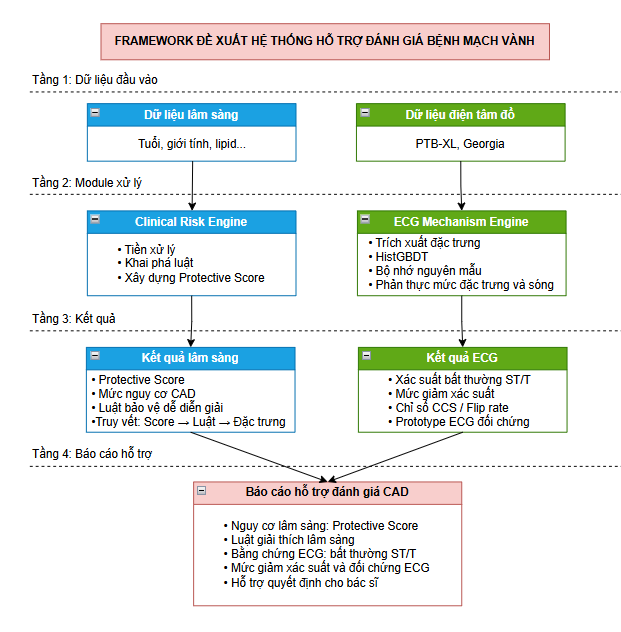
\includegraphics[width=\linewidth]{figure_system_architecture.png}
    \caption{Framework đề xuất của hệ thống hỗ trợ đánh giá bệnh mạch vành đa nguồn dữ liệu, gồm bốn tầng từ tiếp nhận dữ liệu đến lớp ứng dụng hỗ trợ quyết định lâm sàng. Thành phần phân tầng nguy cơ CAD bằng khai phá luật kết hợp và \textit{protective score} (nhánh xanh dương) khai thác dữ liệu lâm sàng dạng bảng theo hướng diễn giải được. Thành phần kiểm chứng cơ chế ST/T trên ECG bằng bộ nhớ nguyên mẫu phản thực (nhánh xanh lá) phân tích và kiểm chứng cơ chế bất thường ECG ST/T theo hướng phản thực. Kết quả của hai thành phần được tổng hợp thành báo cáo hỗ trợ đánh giá cho bác sĩ ở các tầng phía trên.}
    \label{fig:system_architecture}
\end{figure}

\blocksep

Trong phạm vi khóa luận, hai thành phần phân tích nêu trên cùng các quy trình thực nghiệm tương ứng được hiện thực hóa trực tiếp ở mức nghiên cứu. Các tầng tích hợp báo cáo và lớp ứng dụng được mô tả ở mức framework nhằm làm rõ cách đặt các bằng chứng từ dữ liệu lâm sàng và dữ liệu ECG trong cùng một khung hỗ trợ đánh giá.

\blocksep
\noindent{\Large \textbf{Đối tượng và phương pháp nghiên cứu}}

\blocksep

Đối tượng nghiên cứu của khóa luận gồm hai nhóm dữ liệu và hai lớp bài toán bổ sung cho nhau. Nhóm thứ nhất là dữ liệu lâm sàng dạng bảng liên quan đến CAD, được sử dụng để nghiên cứu bài toán phân tầng nguy cơ và rút trích tri thức có khả năng diễn giải. Nhóm thứ hai là dữ liệu ECG 12 chuyển đạo, được sử dụng để nghiên cứu bài toán nhận diện và kiểm chứng cơ chế bất thường ST/T như một nguồn bằng chứng tín hiệu hỗ trợ cho đánh giá tim mạch liên quan đến CAD.

\blocksep

Về phương pháp, khóa luận kết hợp hai hướng tiếp cận. Với dữ liệu lâm sàng, phương pháp chính gồm tiền xử lý, rời rạc hóa, khai phá luật kết hợp và xây dựng \textit{protective score}, sau đó đánh giá bằng cross-validation theo cơ chế không rò rỉ thông tin. Với dữ liệu ECG, phương pháp chính gồm trích xuất đặc trưng điện tâm đồ, huấn luyện mô hình phân loại và kiểm chứng cơ chế bằng phản thực mức đặc trưng, phản thực mức dạng sóng, đối chứng âm tính, quan hệ liều -- đáp ứng và xác thực ngoại bộ. Trên toàn bộ khóa luận, quá trình nghiên cứu được triển khai theo hướng thực nghiệm định lượng, đồng thời đối chiếu kết quả với trực giác lâm sàng và yêu cầu về tính diễn giải.

\blocksep
\noindent{\Large \textbf{Mục tiêu nghiên cứu}}

\blocksep

Khóa luận hướng tới bốn mục tiêu nghiên cứu chính. Thứ nhất, đề xuất framework hệ thống hỗ trợ đánh giá bệnh động mạch vành theo hướng đa nguồn dữ liệu, kết hợp dữ liệu lâm sàng dạng bảng và dữ liệu ECG. Thứ hai, đề xuất một quy trình khai phá luật kết hợp trên dữ liệu lâm sàng nhằm xây dựng thang điểm phân tầng nguy cơ có khả năng diễn giải. Thứ ba, xây dựng mô hình kiểm chứng cơ chế ST/T trên ECG bằng bộ nhớ nguyên mẫu phản thực, xem cơ chế này như một tín hiệu sinh học hỗ trợ cho đánh giá nguy cơ tim mạch liên quan đến CAD. Thứ tư, đánh giá mức độ hợp lý, tính nhất quán và giá trị hỗ trợ chuyên môn của hai pha nghiên cứu thông qua các thí nghiệm định lượng phù hợp.

\blocksep
\noindent{\Large \textbf{Đóng góp của đề tài}}
\blocksep

Các đóng góp chính của khóa luận bao gồm ba hướng.

Thứ nhất, đề xuất framework hệ thống và khung nghiên cứu hai pha cho bài toán hỗ trợ đánh giá bệnh động mạch vành, trong đó mỗi pha khai thác một nguồn dữ liệu khác nhau nhưng cùng hướng tới mục tiêu tăng cường tính diễn giải và giá trị hỗ trợ thực tiễn.

Thứ hai, xây dựng quy trình xử lý dữ liệu lâm sàng bao gồm tiền xử lý, rời rạc hóa, khai phá luật kết hợp và xây dựng \textit{protective score} phục vụ phân tầng nguy cơ, cùng với đánh giá không rò rỉ thông tin nhằm kiểm tra độ ổn định của các luật.

Thứ ba, xây dựng thành phần kiểm chứng cơ chế ST/T trên ECG theo hướng \textit{lưu trữ nguyên mẫu phản thực có định hướng lâm sàng} và thực hiện các thí nghiệm kiểm chứng theo nhiều lớp bằng chứng, bao gồm đánh giá nội bộ, kiểm chứng ngoại bộ và phản thực ở mức đặc trưng lẫn mức dạng sóng, nhằm làm rõ tính hợp lý cơ chế của mô hình.

\blocksep
\noindent{\Large \textbf{Phạm vi và giới hạn của đề tài}}
\blocksep

Khóa luận tập trung vào bài toán \textit{hỗ trợ đánh giá} bệnh động mạch vành, không đặt mục tiêu thay thế hoàn toàn quy trình chẩn đoán lâm sàng. Về mặt hệ thống, phạm vi chính của khóa luận là đề xuất framework tổng thể và hiện thực hai thành phần phân tích cốt lõi của framework đó. Trong đó, pha thứ nhất hiện thực thành phần phân tầng nguy cơ CAD từ dữ liệu lâm sàng bằng khai phá luật kết hợp và \textit{protective score}. Pha thứ hai hiện thực thành phần kiểm chứng cơ chế bất thường ST/T trên ECG bằng bộ nhớ nguyên mẫu phản thực và các phép thử phản thực đa mức. Vì vậy, kết quả của pha thứ hai không được hiểu như một kết luận chẩn đoán xác định bệnh động mạch vành chỉ từ ECG, mà được xem là bằng chứng hỗ trợ về mặt cơ chế, tính nhất quán tín hiệu và khả năng giải thích của mô hình. Các tầng tích hợp báo cáo và lớp ứng dụng cuối chỉ được mô tả ở mức framework đề xuất, không phải trọng tâm hiện thực hóa của khóa luận.

\blocksep
\noindent{\Large \textbf{Bố cục của khóa luận}}
\blocksep

Nội dung của khóa luận được trình bày như sau.

Phần \textit{Mở đầu} trình bày lý do chọn đề tài, mục tiêu nghiên cứu, các đóng góp chính, phạm vi nghiên cứu và bố cục của khóa luận.

\textit{Chương 1. Cơ sở lý thuyết và các nghiên cứu liên quan} trình bày nền tảng về bệnh động mạch vành, phân tầng nguy cơ lâm sàng, vai trò của ECG trong đánh giá tim mạch, học máy diễn giải được và các hướng nghiên cứu liên quan.

\textit{Chương 2. Mô-đun phân tầng nguy cơ CAD từ dữ liệu lâm sàng bằng khai phá luật kết hợp và protective score} trình bày dữ liệu sử dụng, quy trình tiền xử lý, khai phá luật kết hợp, xây dựng protective score và phương pháp đánh giá.

\textit{Chương 3. Mô-đun kiểm chứng cơ chế ST/T trên ECG bằng bộ nhớ nguyên mẫu phản thực} trình bày bài toán nghiên cứu, dữ liệu ECG, đặc trưng sử dụng, mô hình phân tích và cơ chế phản thực dùng để kiểm chứng vai trò của bất thường ST/T.

\textit{Chương 4. Thực nghiệm và đánh giá} trình bày thiết lập thực nghiệm và các kết quả đánh giá của hai pha nghiên cứu, đồng thời thảo luận ý nghĩa và giới hạn của các kết quả thu được.

Phần \textit{Kết luận} tổng kết các kết quả đạt được, nêu ra những hạn chế còn tồn tại và đề xuất các hướng phát triển tiếp theo.

\renewcommand{\thefigure}{\thechapter.\arabic{figure}}
\renewcommand{\thetable}{\thechapter.\arabic{table}}

\newpage
\clearpage
\phantomsection

\setcounter{chapter}{0}
\chapter[{CƠ SỞ LÝ THUYẾT VÀ CÁC NGHIÊN CỨU LIÊN QUAN}]{Cơ sở lý thuyết và các nghiên cứu liên quan}

Chương này trình bày cơ sở lý thuyết và các hướng nghiên cứu liên quan làm nền tảng cho khóa luận. Trọng tâm của chương là làm rõ bối cảnh của bài toán đánh giá bệnh động mạch vành, vai trò của dữ liệu lâm sàng dạng bảng trong phân tầng nguy cơ, vai trò của tín hiệu điện tâm đồ trong phản ánh bất thường điện học liên quan đến nguy cơ tim mạch, cũng như yêu cầu về tính diễn giải và độ tin cậy của các mô hình học máy trong y sinh.

\blocksep

Bên cạnh việc tổng hợp các phương pháp nền tảng, chương này cũng chỉ ra khoảng trống giữa các mô hình dự đoán thuần túy và nhu cầu hỗ trợ chuyên môn trong thực hành lâm sàng. Từ đó, chương làm rõ động lực cho hướng tiếp cận của khóa luận: pha nghiên cứu thứ nhất tập trung vào dữ liệu lâm sàng để xây dựng thang điểm phân tầng nguy cơ có khả năng diễn giải, trong khi pha nghiên cứu thứ hai tập trung vào dữ liệu ECG để kiểm chứng cơ chế bất thường ST/T bằng phản thực và xác thực trên dữ liệu ngoại bộ.

\blocksep

\section{Bài toán hỗ trợ đánh giá bệnh động mạch vành đa nguồn dữ liệu}

\blocksep

Bệnh động mạch vành (Coronary Artery Disease -- CAD) là một trong những nguyên nhân hàng đầu gây tử vong và tàn tật trên toàn thế giới \cite{Libby2011}. Trong thực hành lâm sàng, việc đánh giá nguy cơ CAD có ý nghĩa quan trọng không chỉ ở giai đoạn sàng lọc ban đầu mà còn trong chỉ định xét nghiệm, lựa chọn chiến lược theo dõi và quyết định can thiệp. Tuy nhiên, CAD là một bệnh lý có cơ chế phức tạp, biểu hiện lâm sàng đa dạng và thường không thể được đánh giá đầy đủ chỉ từ một nguồn dữ liệu đơn lẻ.

\blocksep

Thông tin phục vụ đánh giá người bệnh thường đến từ nhiều nguồn khác nhau. Dữ liệu lâm sàng dạng bảng chứa các yếu tố nguy cơ nền như tuổi, giới tính, tiền sử bệnh, đau ngực, huyết áp, lipid máu hoặc đái tháo đường. Đây là những thông tin có giá trị cao trong phân tầng nguy cơ và phù hợp với các công cụ hỗ trợ quyết định dạng điểm số. Trong khi đó, dữ liệu điện tâm đồ (ECG) phản ánh hoạt động điện học của tim theo thời gian, cho phép quan sát các bất thường chức năng mà dữ liệu tĩnh dạng bảng khó thể hiện đầy đủ \cite{Clifford2006}.

\blocksep

Vì vậy, một cách nhìn phù hợp trong bối cảnh hiện nay là xem bài toán như một hệ thống hỗ trợ đánh giá đa nguồn dữ liệu. Theo cách tiếp cận này, dữ liệu lâm sàng và dữ liệu ECG không nhất thiết phải bị ép vào cùng một mô hình duy nhất. Thay vào đó, hai nguồn dữ liệu có thể được đặt trong cùng một framework hỗ trợ đánh giá nhưng được xử lý bởi các mô-đun chuyên biệt. Khi đó, dữ liệu lâm sàng hỗ trợ phân tầng nguy cơ CAD ở mức khái quát, còn dữ liệu ECG hỗ trợ nhận diện và kiểm chứng các cơ chế bất thường điện học có ý nghĩa lâm sàng đối với đánh giá nguy cơ tim mạch.

\blocksep

Trong y sinh, một hệ thống hỗ trợ có giá trị không chỉ cần đạt hiệu năng dự đoán tốt mà còn phải tạo ra được bằng chứng đủ rõ để bác sĩ có thể sử dụng trong bối cảnh ra quyết định thực tế \cite{Topol2019}. Vì vậy, bên cạnh hiệu năng, các khía cạnh như tính diễn giải, độ tin cậy, tính nhất quán khi chuyển sang dữ liệu ngoại bộ và khả năng làm rõ cơ chế tín hiệu là những tiêu chí đặc biệt quan trọng đối với các nghiên cứu theo hướng ứng dụng lâm sàng.

\blocksep

\section{Phân tầng nguy cơ bệnh động mạch vành từ dữ liệu lâm sàng}

\blocksep

\subsection{Các thang điểm nguy cơ truyền thống}

\blocksep

Đánh giá nguy cơ tim mạch từ dữ liệu lâm sàng là một hướng nghiên cứu lâu đời và có nền tảng vững chắc trong y học thực chứng. Một trong những cách tiếp cận sớm là sử dụng các thang điểm hoặc mô hình xác suất dựa trên các biến lâm sàng cơ bản. Ví dụ điển hình là mô hình Diamond--Forrester, trong đó tuổi, giới tính và kiểu đau ngực được sử dụng để ước lượng xác suất mắc CAD trước xét nghiệm \cite{Diamond1979}. Cách tiếp cận này có ưu điểm là đơn giản, dễ sử dụng và gần với tư duy ra quyết định lâm sàng.

\blocksep

Ở phạm vi nguy cơ tim mạch rộng hơn, các thang điểm như Framingham Risk Score và SCORE được phát triển nhằm ước lượng xác suất biến cố tim mạch trong trung và dài hạn dựa trên các yếu tố nguy cơ như huyết áp, cholesterol, hút thuốc và đái tháo đường \cite{DAgostino2008, Conroy2003}. Các thang điểm này đã được xác thực trên nhiều quần thể và giữ vai trò quan trọng trong các hướng dẫn lâm sàng.

\blocksep

Tuy nhiên, các mô hình truyền thống cũng có những hạn chế rõ ràng. Thứ nhất, chúng thường dựa trên số lượng biến đầu vào hạn chế và giả định cấu trúc quan hệ tương đối đơn giản giữa các yếu tố nguy cơ. Thứ hai, hiệu năng của các thang điểm có thể giảm khi áp dụng sang quần thể khác hoặc khi dữ liệu đầu vào bị thiếu hụt. Thứ ba, chúng khó nắm bắt các tổ hợp đặc trưng phức tạp hoặc các mẫu hình hiếm gặp nhưng có ý nghĩa đối với phân tầng nguy cơ \cite{Krittanawong2017}.

\blocksep

\subsection{Các phương pháp học máy trên dữ liệu lâm sàng dạng bảng}

\blocksep

Sự phát triển của học máy mở ra khả năng xây dựng các mô hình dự đoán linh hoạt hơn trên dữ liệu lâm sàng dạng bảng. Nhiều thuật toán như logistic regression mở rộng, cây quyết định, random forest, gradient boosting hoặc các mô hình tổ hợp có thể khai thác tốt hơn mối quan hệ phi tuyến và tương tác giữa nhiều biến lâm sàng \cite{Krittanawong2017}. Trong nhiều trường hợp, các mô hình này cho hiệu năng tốt hơn so với các thang điểm truyền thống khi được huấn luyện và đánh giá cẩn thận.

\blocksep

Tuy nhiên, hiệu năng cao không đồng nghĩa với giá trị hỗ trợ lâm sàng cao. Các mô hình phức tạp thường khó giải thích hơn, đặc biệt khi sử dụng nhiều biến đầu vào có tương quan chồng lấp. Trong các ứng dụng liên quan đến phân tầng nguy cơ, bác sĩ không chỉ quan tâm đến nhãn đầu ra mà còn cần biết yếu tố nào đóng vai trò bảo vệ, yếu tố nào đi kèm nguy cơ cao, và mẫu hình nào lặp lại đủ ổn định để có thể sử dụng trong thực hành \cite{Lipton2018, Rudin2019}.

\blocksep

Vì vậy, một hướng đi quan trọng là kết hợp sức mạnh của học máy với các hình thức biểu diễn tri thức dễ hiểu hơn. Trong khóa luận này, dữ liệu lâm sàng không được sử dụng chủ yếu để xây dựng một bộ phân loại “hộp đen”, mà được khai thác nhằm rút ra các luật kết hợp có ý nghĩa và tổng hợp chúng thành một thang điểm phân tầng nguy cơ. Cách tiếp cận này phù hợp với đặc điểm của pha nghiên cứu thứ nhất, nơi mục tiêu trọng tâm là tri thức diễn giải được và đánh giá không rò rỉ thông tin, thay vì theo đuổi tối đa một chỉ số phân loại duy nhất.

\blocksep

\subsection{Khai phá luật kết hợp và thang điểm diễn giải được}

\blocksep

Khai phá luật kết hợp là một kỹ thuật quan trọng trong khai phá dữ liệu, nhằm phát hiện các mối đồng xuất hiện có ý nghĩa giữa các thuộc tính trong dữ liệu \cite{Lavrac1999}. Trong bối cảnh y sinh, luật kết hợp có thể được hiểu như các quy tắc dạng “nếu--thì”, trong đó một tổ hợp dấu hiệu hoặc yếu tố nguy cơ đi kèm với xác suất cao hơn hoặc thấp hơn của một tình trạng bệnh. Ưu điểm lớn nhất của biểu diễn này là tính minh bạch: tri thức được thể hiện ở mức gần với lập luận của con người hơn so với các vector trọng số trừu tượng của một mô hình phức tạp.

\blocksep

Khi áp dụng vào dữ liệu lâm sàng, quy trình khai phá luật thường bao gồm các bước tiền xử lý như xử lý thiếu dữ liệu, rời rạc hóa biến liên tục và mã hóa dữ liệu thành dạng phù hợp với việc sinh luật. Sau đó, các luật được đánh giá theo các độ đo như độ hỗ trợ, độ tin cậy và lift hoặc các tiêu chí thống nhất khác nhằm lọc ra những luật có đủ độ mạnh và tính ổn định \cite{Lavrac1999}. Tuy nhiên, số lượng luật có thể tăng rất nhanh, dẫn đến hiện tượng dư thừa và khó diễn giải nếu không có chiến lược chọn lọc thích hợp.

\blocksep

Một hướng thực dụng là không sử dụng toàn bộ tập luật như đầu ra cuối cùng, mà tổng hợp chúng thành một chỉ số hoặc thang điểm phân tầng nguy cơ. Cách làm này vừa giữ lại được tri thức diễn giải được, vừa giúp phương pháp dễ sử dụng hơn trong thực tế. Đây cũng là lý do pha nghiên cứu thứ nhất lựa chọn xây dựng \textit{protective score} từ các đặc trưng lâm sàng khớp với các luật ổn định, thay vì chỉ so sánh đơn thuần các mô hình phân loại chuẩn.

\blocksep

\section{Vai trò của điện tâm đồ và bất thường ST/T trong đánh giá nguy cơ tim mạch}

\blocksep

Điện tâm đồ là một trong những tín hiệu sinh lý cơ bản nhất trong tim mạch học, phản ánh hoạt động điện học của tim qua các pha khử cực và tái cực \cite{Clifford2006}. ECG có ưu điểm là không xâm lấn, chi phí thấp, dễ thu nhận và đã được sử dụng rộng rãi trong đánh giá nhiều tình trạng tim mạch khác nhau. Trong bối cảnh hỗ trợ đánh giá nguy cơ tim mạch, ECG có thể cung cấp tín hiệu bổ sung quan trọng bên cạnh dữ liệu lâm sàng, đặc biệt khi quan tâm đến các bất thường điện học liên quan đến thiếu máu cơ tim hoặc tái cực thất.

\blocksep

Trong một chu kỳ ECG điển hình, các thành phần như sóng P, phức bộ QRS, đoạn ST và sóng T tương ứng với các giai đoạn khác nhau của hoạt động điện tim. Trong số đó, đoạn ST và sóng T thường được xem là những vùng nhạy cảm với các thay đổi liên quan đến tái cực thất và thiếu máu cục bộ cơ tim \cite{Clifford2006}. Vì vậy, các bất thường ST/T từ lâu đã được coi là một nguồn tín hiệu lâm sàng quan trọng trong đánh giá tim mạch, dù không đồng nhất hoàn toàn với chẩn đoán xác định CAD.

\blocksep

Điều cần phân biệt ở đây là “tín hiệu liên quan về mặt cơ chế” không đồng nhất với “nhãn chẩn đoán cuối cùng”. Một mô hình ECG có thể học được cơ chế bất thường ST/T một cách nhất quán và có ý nghĩa lâm sàng, nhưng điều đó không đồng nghĩa với việc mô hình đó trực tiếp chẩn đoán bệnh động mạch vành ở mức xác định. Trong khóa luận này, vai trò của pha nghiên cứu thứ hai được đặt đúng ở mức đó: phân tích và kiểm chứng một cơ chế tín hiệu ECG hỗ trợ cho đánh giá nguy cơ tim mạch liên quan đến CAD, chứ không thay thế quy trình chẩn đoán lâm sàng chuẩn.

\blocksep

Từ góc nhìn học máy, ECG là một nguồn dữ liệu giàu cấu trúc hơn nhiều so với dữ liệu dạng bảng. Một mặt, điều này cho phép mô hình khai thác những mẫu hình tinh vi; mặt khác, nó làm tăng nguy cơ mô hình học nhầm các dấu hiệu không bền vững hoặc khó giải thích. Vì vậy, nếu chỉ dừng ở việc báo cáo hiệu năng phân loại trên ECG, giá trị hỗ trợ chuyên môn của mô hình vẫn còn hạn chế. Cần có những phương pháp cho phép kiểm tra xem mô hình thực sự đang dựa vào thành phần tín hiệu nào và liệu các thành phần đó có phù hợp với kỳ vọng lâm sàng hay không.

\blocksep

\section{Học máy diễn giải được và độ tin cậy trong y sinh}

\blocksep

\subsection{Hiệu năng dự đoán và giới hạn của các chỉ số tổng quát}

\blocksep

Trong các nghiên cứu học máy y sinh, hiệu năng dự đoán thường được lượng hóa bằng các chỉ số như accuracy, ROC-AUC, PR-AUC, balanced accuracy hoặc F1-score. Các chỉ số này cần thiết để đo khả năng phân biệt giữa các nhóm nhãn, nhưng chúng không tự động bảo đảm rằng mô hình phù hợp với nhu cầu sử dụng lâm sàng \cite{Topol2019}. Một mô hình có AUC cao vẫn có thể thiếu minh bạch, thiếu ổn định khi chuyển miền dữ liệu hoặc khai thác những tín hiệu không mong muốn.

\blocksep

Vì vậy, trong các bài toán rủi ro cao, đánh giá mô hình cần vượt ra ngoài một bảng điểm hiệu năng thuần túy. Đối với dữ liệu lâm sàng, điều quan trọng là tri thức rút ra có ổn định qua các lần chia dữ liệu hay không. Đối với dữ liệu ECG, điều quan trọng là cơ chế tín hiệu mà mô hình đang sử dụng có còn nhất quán khi chuyển sang dữ liệu ngoại bộ hay không. Đây cũng là lý do pha nghiên cứu thứ hai không được định vị như một nghiên cứu theo đuổi “hiệu năng phân loại cao nhất”, mà như một nghiên cứu \textit{kiểm chứng cơ chế} với nhiều lớp đánh giá bổ sung.

\blocksep

\subsection{Tính diễn giải và nhu cầu minh bạch}

\blocksep

Tính diễn giải là một yêu cầu cốt lõi trong các hệ thống học máy y sinh \cite{Lipton2018}. Trong môi trường lâm sàng, mô hình không chỉ cần đưa ra một dự đoán, mà còn cần cung cấp cơ sở để dự đoán đó có thể được kiểm tra, phản biện và sử dụng cùng với tri thức chuyên môn. Từ góc nhìn này, các mô hình hoặc chỉ số diễn giải được thường có ưu thế rõ ràng so với các kiến trúc “hộp đen” khó giải thích \cite{Rudin2019}.

\blocksep

Tính diễn giải có thể đạt được theo nhiều cách khác nhau. Một hướng là sử dụng các mô hình vốn dĩ dễ hiểu, như luật kết hợp hoặc thang điểm nguy cơ. Hướng khác là sử dụng các công cụ hậu giải thích (post-hoc explanation) để phân tích một mô hình mạnh hơn. Tuy nhiên, trong các bài toán y sinh có mức độ rủi ro cao, các giải thích hậu nghiệm chỉ thực sự có giá trị khi được kiểm chứng thêm bằng các thí nghiệm cho thấy mô hình phản ứng phù hợp với trực giác lâm sàng.

\blocksep

Trong khóa luận này, tính diễn giải được tiếp cận theo hai cách bổ sung. Pha thứ nhất sử dụng luật kết hợp và thang điểm để biểu diễn tri thức lâm sàng ở mức dễ hiểu. Pha thứ hai sử dụng phân tích phản thực trên ECG để kiểm tra xem mô hình có thực sự đang dựa vào bất thường ST/T hay không. Hai hướng này khác nhau về mặt kỹ thuật, nhưng thống nhất ở mục tiêu chung là tăng giá trị giải thích của hệ thống hỗ trợ đánh giá.

\blocksep

\subsection{Độ tin cậy, hiệu chỉnh và xác thực ngoại bộ}

\blocksep

Ngoài tính diễn giải, độ tin cậy là một tiêu chí không thể thiếu khi xem xét mô hình học máy trong y sinh. Độ tin cậy ở đây bao gồm nhiều khía cạnh: mô hình có ổn định khi chia lại dữ liệu hay không, xác suất dự đoán có được hiệu chỉnh hợp lý hay không, và kết quả có còn giữ được khi chuyển sang dữ liệu độc lập hay không \cite{Guo2017, Quinonero2009}. Trong nhiều trường hợp, một mô hình đạt kết quả tốt trên dữ liệu nội bộ nhưng giảm mạnh khi đánh giá ngoại bộ, cho thấy mô hình đã học những tín hiệu gắn với miền dữ liệu hơn là cơ chế mục tiêu.

\blocksep

Với dữ liệu lâm sàng, yêu cầu cơ bản là đánh giá không rò rỉ thông tin và kiểm tra độ ổn định của luật qua các lần chia dữ liệu hoặc các tập dữ liệu khác nhau. Với dữ liệu ECG, độ tin cậy còn gắn chặt với xác thực ngoại bộ và kiểm tra âm tính. Nếu mô hình chỉ hoạt động trên một bộ dữ liệu duy nhất hoặc không phân biệt được giữa tín hiệu mục tiêu và các vùng tín hiệu đối chứng, thì khó có thể coi đó là bằng chứng đủ mạnh cho giá trị cơ chế của mô hình.

\blocksep

Vì vậy, các thiết kế thí nghiệm dựa trên xác thực ngoại bộ, đối chứng âm tính, khoảng tin cậy bootstrap và nhiều lớp đo lường nhất quán là đặc biệt quan trọng. Đây cũng là nét đặc trưng của pha nghiên cứu thứ hai: không chỉ đánh giá trên PTB-XL nội bộ mà còn kiểm tra lại trên Georgia ngoại bộ, đồng thời so sánh tác động của chỉnh sửa ST/T với các cửa sổ đối chứng như pre-QRS, P/PR hoặc QRS.

\blocksep

\section{Phản thực và kiểm chứng cơ chế trong phân tích ECG}

\blocksep

Trong những năm gần đây, phản thực (giải thích phản thực) nổi lên như một hướng quan trọng trong giải thích mô hình học máy \cite{Wachter2017}. Ý tưởng cốt lõi là thay vì chỉ hỏi “đặc trưng nào quan trọng”, đặt câu hỏi “nếu thay đổi một thành phần cụ thể của đầu vào theo cách có kiểm soát thì dự đoán của mô hình sẽ thay đổi như thế nào”. Trong bối cảnh y sinh, cách đặt câu hỏi này gần với tư duy can thiệp và kiểm chứng cơ chế hơn so với việc chỉ xếp hạng mức độ quan trọng của đặc trưng.

\blocksep

Đối với dữ liệu ECG, phản thực có thể được thực hiện ở nhiều mức khác nhau. Ở mức đặc trưng, có thể chỉnh sửa một nhóm đặc trưng liên quan đến đoạn ST hoặc hình dạng sóng, sau đó đo mức giảm xác suất dự đoán của lớp bệnh. Ở mức dạng sóng, có thể trực tiếp chỉnh sửa một đoạn tín hiệu trên sóng ECG, ví dụ kéo vùng ST/T của một ca bất thường tiến dần về một mẫu bình thường, rồi đánh giá phản ứng của mô hình sau khi trích xuất lại đặc trưng.

\blocksep

Giá trị của phản thực nằm ở chỗ nó có thể tạo ra bằng chứng mạnh hơn so với attribution thuần túy. Nếu mô hình thực sự dựa vào cơ chế ST/T, thì việc chỉnh sửa ST/T theo hướng “bình thường hóa” phải làm giảm xác suất dự đoán lớp bất thường một cách có hệ thống. Hơn nữa, hiệu ứng này cần mạnh hơn đáng kể so với việc chỉnh sửa các vùng đối chứng không phải mục tiêu. Nếu khi tăng cường mức chỉnh sửa mà hiệu ứng cũng tăng theo một quan hệ đơn điệu, điều đó tạo thêm bằng chứng cho tính nhất quán của cơ chế được mô hình học.

\blocksep

Từ góc nhìn đánh giá nghiên cứu, đối chứng âm tính và liều -- đáp ứng là hai công cụ đặc biệt quan trọng. Negative controls cho biết mô hình có đang phản ứng riêng với vùng mục tiêu hay chỉ phản ứng với bất kỳ chỉnh sửa nào trên sóng. Dose-response cho biết hiệu ứng của chỉnh sửa có tăng dần một cách hợp lý khi can thiệp mạnh hơn hay không. Những nguyên tắc này phù hợp trực tiếp với pha nghiên cứu thứ hai, nơi cơ chế ST/T được đánh giá bằng cả phản thực mức đặc trưng, phản thực mức dạng sóng và các cửa sổ đối chứng âm tính.

\blocksep

\section{Khoảng trống nghiên cứu và định hướng của khóa luận}

\blocksep

Từ các phân tích trên có thể thấy rằng các nghiên cứu hiện có thường rơi vào một trong hai hướng. Hướng thứ nhất tập trung vào dữ liệu lâm sàng dạng bảng và xây dựng các công cụ phân tầng nguy cơ, nhưng nhiều phương pháp hoặc còn quá đơn giản để khai thác hết dữ liệu, hoặc quá phức tạp để diễn giải rõ ràng trong thực hành. Hướng thứ hai tập trung vào phân tích ECG bằng các mô hình học máy mạnh, nhưng nhiều nghiên cứu dừng lại ở việc báo cáo hiệu năng phân loại mà chưa cung cấp đủ bằng chứng cho cơ chế tín hiệu mà mô hình đang sử dụng.

\blocksep

Khoảng trống nổi bật ở đây là thiếu một framework hỗ trợ đánh giá có thể kết nối giá trị của hai nguồn dữ liệu này trong cùng một câu chuyện bệnh động mạch vành. Cụ thể, cần có một mô-đun lâm sàng giúp phân tầng nguy cơ theo hướng diễn giải được, và một mô-đun ECG giúp kiểm tra các bất thường điện học theo hướng có thể xác thực bằng phản thực, dữ liệu ngoại bộ và đối chứng âm tính. Khi đó, hệ thống không chỉ đưa ra dự đoán mà còn cung cấp bằng chứng ở cả mức yếu tố lâm sàng và mức cơ chế tín hiệu.

\blocksep

Bảng~\ref{tab:related_comparison} tổng hợp các hướng tiếp cận tiêu biểu trong lĩnh vực và so sánh với phương pháp đề xuất của khóa luận theo bốn tiêu chí chính: nguồn dữ liệu, phương pháp chính, tính diễn giải và mức độ xác thực ngoại bộ.

\blocksep

\begin{table}[H]
\centering
\caption{So sánh phương pháp đề xuất với các hướng tiếp cận liên quan}
\label{tab:related_comparison}
\begin{tabular}{p{0.24\linewidth}C{0.13\linewidth}p{0.20\linewidth}C{0.12\linewidth}p{0.17\linewidth}}
\hline
\textbf{Hướng tiếp cận} & \textbf{Nguồn dữ liệu} & \textbf{Phương pháp chính} & \textbf{Tính diễn giải} & \textbf{Xác thực ngoại bộ} \\
\hline
Thang điểm nguy cơ truyền thống \cite{Diamond1979, DAgostino2008} & Lâm sàng & Score công thức & Cao & Có (theo quần thể) \\
ML trên dữ liệu bảng \cite{Krittanawong2017} & Lâm sàng & Gradient boosting, MLP & Thấp & Thường không \\
Khai phá luật kết hợp đơn giản \cite{Lavrac1999} & Lâm sàng & Apriori, FP-Growth & Cao & Thường không \\
Deep learning trên ECG \cite{Topol2019} & ECG & CNN, LSTM, Transformer & Thấp & Đôi khi \\
XAI hậu nghiệm trên ECG \cite{Lipton2018} & ECG & LIME, SHAP, GradCAM & Trung bình & Hiếm \\
\hline
\textbf{Phương pháp đề xuất} & \textbf{Lâm sàng + ECG} & \textbf{Khai phá luật + bộ nhớ nguyên mẫu phản thực} & \textbf{Cao (hai mức)} & \textbf{Có (Georgia)} \\
\hline
\end{tabular}
\end{table}

\blocksep

Đây cũng chính là định hướng của khóa luận. Trên nền một framework hỗ trợ đánh giá đa nguồn dữ liệu được đề xuất, pha nghiên cứu thứ nhất tập trung vào khai phá luật kết hợp trên dữ liệu CAD dạng bảng để xây dựng \textit{protective score} có khả năng phân tầng nguy cơ và ổn định qua đánh giá chéo không rò rỉ thông tin. Pha nghiên cứu thứ hai tập trung vào bài toán bất thường ST/T trên ECG 12 chuyển đạo, trong đó mô hình được kiểm tra bằng phản thực mức đặc trưng và mức dạng sóng, xác thực ngoại bộ và các đối chứng âm tính nhằm làm rõ tính hợp lý cơ chế của tín hiệu ECG hỗ trợ đánh giá tim mạch. Hai pha này là hai mô-đun phân tích cốt lõi của framework đề xuất, không thay thế nhau mà bổ sung cho nhau trong mục tiêu hỗ trợ đánh giá CAD.

\blocksep

\section{Tổng kết chương}

\blocksep

Chương này đã trình bày các cơ sở lý thuyết và các hướng nghiên cứu liên quan làm nền tảng cho khóa luận. Trước hết, chương đã làm rõ bối cảnh của bài toán hỗ trợ đánh giá bệnh động mạch vành theo hướng đa nguồn dữ liệu, trong đó dữ liệu lâm sàng và dữ liệu ECG giữ những vai trò bổ sung khác nhau. Tiếp theo, chương đã tổng hợp các hướng tiếp cận trong phân tầng nguy cơ CAD từ dữ liệu lâm sàng, đồng thời nhấn mạnh giá trị của các phương pháp diễn giải được như luật kết hợp và thang điểm nguy cơ.

\blocksep

Chương cũng đã phân tích vai trò của ECG, đặc biệt là bất thường ST/T, trong đánh giá nguy cơ tim mạch và chỉ ra nhu cầu phải kiểm chứng cơ chế tín hiệu thay vì chỉ báo cáo hiệu năng phân loại. Đồng thời, các khái niệm về tính diễn giải, độ tin cậy, xác thực ngoại bộ, phản thực, đối chứng âm tính và quan hệ liều -- đáp ứng đã được thảo luận như những tiêu chí quan trọng để đánh giá một mô hình học máy y sinh có giá trị hỗ trợ thực tế.

\blocksep

Trên cơ sở đó, chương làm rõ khoảng trống nghiên cứu mà khóa luận hướng tới: kết hợp một mô-đun lâm sàng có khả năng phân tầng nguy cơ CAD và một mô-đun ECG có khả năng kiểm chứng cơ chế bất thường điện học như một nguồn bằng chứng bổ trợ. Những nội dung này tạo tiền đề cho Chương~2, nơi pha nghiên cứu thứ nhất sẽ được trình bày chi tiết dưới góc nhìn khai phá luật kết hợp và xây dựng thang điểm phân tầng nguy cơ từ dữ liệu lâm sàng.

\newpage
\clearpage
\phantomsection

\setcounter{chapter}{1}
\chapter[{MÔ-ĐUN PHÂN TẦNG NGUY CƠ CAD TỪ DỮ LIỆU LÂM SÀNG BẰNG KHAI PHÁ LUẬT KẾT HỢP VÀ PROTECTIVE SCORE}]{Mô-đun phân tầng nguy cơ CAD từ dữ liệu lâm sàng bằng khai phá luật kết hợp và protective score}

Chương này trình bày chi tiết mô-đun phân tầng nguy cơ CAD từ dữ liệu lâm sàng bằng khai phá luật kết hợp và \textit{protective score}, tương ứng với pha nghiên cứu thứ nhất của khóa luận. Khác với các hướng tiếp cận chủ yếu nhấn mạnh vào hiệu năng phân loại, pha nghiên cứu này tập trung vào việc rút trích tri thức trực tiếp từ dữ liệu và tổng hợp tri thức đó thành một thang điểm có thể diễn giải trong bối cảnh lâm sàng.

\blocksep

Về mặt thực nghiệm, pha nghiên cứu thứ nhất được tổ chức quanh bốn thành phần chính: tiền xử lý dữ liệu lâm sàng, khai phá luật kết hợp trong từng lần chia dữ liệu đánh giá chéo, xây dựng \textit{protective score} từ các luật bảo vệ và đánh giá độ ổn định cũng như giá trị phân tầng nguy cơ của thang điểm thu được. Cách tiếp cận này phù hợp với mục tiêu của khóa luận, vì nó cho phép kết nối dữ liệu, tri thức lâm sàng và quy trình đánh giá một cách minh bạch hơn so với việc chỉ huấn luyện một bộ phân loại khó diễn giải, đồng thời vẫn bám sát bài toán CAD.

\blocksep

\section{Tổng quan pha nghiên cứu thứ nhất}

\blocksep

Pha nghiên cứu thứ nhất được thiết kế như một mô-đun hỗ trợ đánh giá nguy cơ CAD từ dữ liệu lâm sàng. Đầu vào của mô-đun là các thuộc tính lâm sàng và cận lâm sàng đã được chuẩn hóa về cùng định dạng, bao gồm cả biến liên tục và biến phân loại. Đầu ra của mô-đun không phải là một xác suất dự đoán duy nhất, mà là một chỉ số phân tầng nguy cơ có thể giải thích thông qua các luật kết hợp rút ra từ dữ liệu.

\blocksep

Ý tưởng trung tâm của pha nghiên cứu này là thay vì chỉ hỏi mô hình “dự đoán bệnh hay không bệnh”, xây dựng một thang điểm phản ánh mức độ hiện diện của các dấu hiệu gắn với nhóm nguy cơ thấp hoặc nhóm không CAD. Nếu một bệnh nhân thỏa mãn nhiều quy tắc bảo vệ ổn định, bệnh nhân đó sẽ nhận \textit{protective score} cao hơn và có xu hướng thuộc nhóm nguy cơ thấp hơn. Cách tiếp cận này gần với tư duy phân tầng trong thực hành lâm sàng, nơi người bệnh thường được xếp theo mức nguy cơ thay vì chỉ nhận một nhãn nhị phân.

\blocksep

Toàn bộ quy trình của pha nghiên cứu thứ nhất được tóm tắt trong Hình~\ref{fig:phase1_pipeline}. Quy trình bắt đầu từ dữ liệu lâm sàng thô, sau đó trải qua các bước tiền xử lý, rời rạc hóa và mã hóa one-hot. Trên dữ liệu đã mã hóa, các luật kết hợp được khai phá trong từng tập huấn luyện, tách thành luật liên quan đến CAD và luật liên quan đến nhóm bảo vệ. Từ tập luật bảo vệ, một \textit{protective score} được xây dựng theo nguyên tắc đếm các nhóm đặc trưng lâm sàng độc nhất đã khớp, rồi được sử dụng để phân tầng nguy cơ và đánh giá.

\blocksep

\begin{figure}[H]
    \centering
    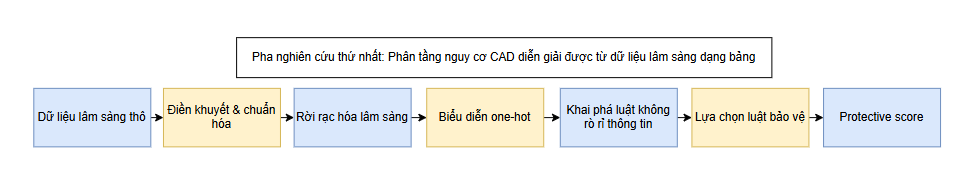
\includegraphics[width=0.95\linewidth]{figure_phase1_pipeline.png}
    \caption{Pipeline tổng thể của pha nghiên cứu thứ nhất.}
    \label{fig:phase1_pipeline}
\end{figure}

\section{Dữ liệu sử dụng và tiền xử lý}

\blocksep

\subsection{Bộ dữ liệu sử dụng}

\blocksep

Pha nghiên cứu thứ nhất sử dụng ba bộ dữ liệu lâm sàng liên quan đến CAD. Bộ dữ liệu chính là Z-Alizadeh Sani, gồm 303 ca với 55 thuộc tính gốc và nhãn chẩn đoán dựa trên kết quả chụp mạch vành \cite{AlizadehSani2013}. Đây là bộ dữ liệu có mức độ chi tiết cao, bao gồm các biến nhân khẩu học, triệu chứng lâm sàng, yếu tố nguy cơ nền, xét nghiệm máu và một số chỉ số tim mạch chức năng. Trong pha nghiên cứu này, Z-Alizadeh được xem là nguồn dữ liệu trọng tâm để xây dựng và kiểm tra tính hợp lý của \textit{protective score}.

\blocksep

Hai bộ dữ liệu còn lại là UCI Cleveland và UCI Hungarian \cite{Detrano1989}, đều được chuyển về nhãn nhị phân CAD thông qua biến \texttt{Num > 0}. Mỗi bộ dữ liệu có quy mô khoảng 300 ca, số thuộc tính gốc ít hơn Z-Alizadeh nhưng vẫn có vai trò quan trọng trong việc kiểm tra khả năng tổng quát hóa của phương pháp. Việc sử dụng đồng thời ba bộ dữ liệu giúp hạn chế nguy cơ rút ra kết luận chỉ từ một cấu trúc dữ liệu đơn lẻ và tạo điều kiện đánh giá phương pháp trên những miền lâm sàng khác nhau.

\blocksep

Trong pha nghiên cứu thứ nhất, thống kê tổng quát cho ba bộ dữ liệu như sau:

\renewcommand{\labelitemi}{$+$}
\begin{itemize}
	\item Z-Alizadeh: 303 mẫu, tỷ lệ CAD khoảng 71.3\%, 55 thuộc tính gốc.
	\item UCI Cleveland: 303 mẫu, tỷ lệ CAD khoảng 45.9\%, 13 thuộc tính gốc.
	\item UCI Hungarian: 294 mẫu, tỷ lệ CAD khoảng 36.1\%, 13 thuộc tính gốc.
\end{itemize}

\blocksep

Bảng~\ref{tab:phase1_datasets} tổng hợp đặc điểm chính của ba bộ dữ liệu theo định dạng so sánh, bao gồm quy mô mẫu, tỷ lệ dương tính, số thuộc tính gốc trước khi tiền xử lý và cách gán nhãn lâm sàng.

\blocksep

\begin{table}[H]
\centering
\caption{Đặc điểm tổng quát của ba bộ dữ liệu lâm sàng trong pha nghiên cứu thứ nhất}
\label{tab:phase1_datasets}
\begin{tabular}{p{0.24\linewidth}C{0.12\linewidth}C{0.14\linewidth}C{0.18\linewidth}p{0.20\linewidth}}
\hline
\textbf{Bộ dữ liệu} & \textbf{Số mẫu} & \textbf{Tỷ lệ CAD} & \textbf{Số thuộc tính gốc} & \textbf{Cách gán nhãn} \\
\hline
Z-Alizadeh Sani & 303 & 71.3\% & 55 & Kết quả chụp mạch vành \\
UCI Cleveland & 303 & 45.9\% & 13 & \texttt{Num > 0} \\
UCI Hungarian & 294 & 36.1\% & 13 & \texttt{Num > 0} \\
\hline
\end{tabular}
\end{table}

\blocksep

\subsection{Xử lý dữ liệu thiếu và chuẩn hóa dữ liệu}

\blocksep

Dữ liệu lâm sàng trong thực tế thường tồn tại giá trị thiếu hoặc khác biệt về cách mã hóa giữa các bộ dữ liệu. Vì vậy, bước tiền xử lý được thiết kế theo hướng đơn giản nhưng ổn định. Với các biến số, giá trị thiếu được thay bằng trung vị của cột; với các biến phân loại, giá trị thiếu được thay bằng mode. Lựa chọn này giúp giảm ảnh hưởng của ngoại lai và tránh đưa thêm những giả định quá mạnh vào dữ liệu.

\blocksep

Đối với Z-Alizadeh, các biến nhị phân hoặc dạng yes/no được chuẩn hóa về dạng 0/1. Một số trường hợp mã hóa không đồng nhất như \texttt{Fmale}, \texttt{female} hoặc \texttt{male} cũng được chuẩn hóa lại trước khi sử dụng. Đối với UCI Cleveland và UCI Hungarian, toàn bộ các cột được ép về kiểu số, ký hiệu \texttt{?} được xử lý như dữ liệu thiếu, sau đó nhãn \texttt{Cath} được sinh từ biến \texttt{Num}. Nhờ vậy, cả ba bộ dữ liệu đều được đưa về cùng một đích biểu diễn: các mẫu lâm sàng với nhãn nhị phân CAD/Normal.

\blocksep

\subsection{Rời rạc hóa các biến liên tục}

\blocksep

Do khai phá luật kết hợp hoạt động hiệu quả nhất trên dữ liệu rời rạc, các biến liên tục được chuyển thành các khoảng giá trị có ý nghĩa lâm sàng. Trong chương trình thực nghiệm của pha nghiên cứu thứ nhất, tập ngưỡng rời rạc hóa được khai báo rõ trong \texttt{cad\_tabular\_config.py} dưới hai cấu hình riêng cho Z-Alizadeh và UCI.

\blocksep

Với Z-Alizadeh, các biến như tuổi, BMI, huyết áp, đường huyết đói, LDL, HDL, triglyceride hoặc phân suất tống máu được chia thành các mức như \texttt{young/mid/old}, \texttt{normal/over/obese}, \texttt{optimal/high}, \texttt{poor/mid/good}. Với UCI, các biến như huyết áp nghỉ, cholesterol, nhịp tim cực đại và \texttt{oldpeak} cũng được rời rạc hóa thành các mức có thể diễn giải theo lâm sàng.

\blocksep

Rời rạc hóa theo ngưỡng có hai vai trò chính. Thứ nhất, nó đưa dữ liệu về dạng phù hợp với khai phá luật. Thứ hai, nó làm tăng khả năng diễn giải của luật thu được, vì mỗi điều kiện trong luật tương ứng với một trạng thái y sinh có thể hiểu được, thay vì một giá trị liên tục khó sử dụng trực tiếp trong lập luận lâm sàng.

\blocksep

\subsection{Mã hóa one-hot và biểu diễn giao dịch}

\blocksep

Sau bước rời rạc hóa, mỗi mẫu bệnh nhân được chuyển thành một bản ghi gồm các mục (items), trong đó mỗi mục biểu diễn một trạng thái cụ thể của một thuộc tính, chẳng hạn như \texttt{Age\_bin\_old}, \texttt{LDL\_bin\_high} hoặc \texttt{Typical Chest Pain\_1}. Tiếp theo, dữ liệu được mã hóa one-hot để tạo ra ma trận nhị phân phục vụ khai phá luật.

\blocksep

Trong biểu diễn này, mỗi hàng tương ứng với một bệnh nhân và mỗi cột tương ứng với một item. Với Z-Alizadeh, số item sau mã hóa là 107; với Cleveland là 42; với Hungarian là 39. Cách biểu diễn này cho phép xem mỗi bệnh nhân như một “giao dịch” trong bài toán khai phá luật kết hợp, còn các yếu tố lâm sàng là những mục xuất hiện trong giao dịch đó.

\blocksep

Một chi tiết quan trọng là nhãn cũng được đưa vào dữ liệu dưới dạng hai item đặc biệt: \texttt{Cath\_Cad\_Y} và \texttt{Cath\_Normal\_Y}. Tuy nhiên, trong khai phá luật, các item này chỉ được phép xuất hiện ở vế kết luận, không được xuất hiện ở vế điều kiện. Ràng buộc này bảo đảm rằng các luật thực sự biểu diễn mối liên hệ từ đặc trưng lâm sàng đến tình trạng bệnh, thay vì làm rò rỉ nhãn vào điều kiện.

\blocksep

\section{Khai phá luật kết hợp}

\blocksep

\subsection{Thuật toán và các tham số chính}

\blocksep

Trong pha nghiên cứu thứ nhất, các luật kết hợp được khai phá bằng thuật toán Apriori \cite{Agrawal1994} thông qua thư viện \texttt{mlxtend} \cite{Raschka2018}. Thuật toán được cấu hình theo các tham số chính sau:

\renewcommand{\labelitemi}{$+$}
\begin{itemize}
	\item \texttt{min\_support = 0.06}
	\item \texttt{min\_confidence = 0.60}
	\item \texttt{min\_lift = 1.40}
	\item \texttt{max\_len = 3}
	\item \texttt{top\_n\_rules = 10}
	\item \texttt{threshold = 2}
	\item \texttt{n\_splits = 5}
\end{itemize}

\blocksep

Ngưỡng \texttt{support} giúp loại bỏ các mẫu hình quá hiếm; \texttt{confidence} bảo đảm độ mạnh của luật; \texttt{lift} giúp loại bỏ các luật có thể xuất hiện do ngẫu nhiên; còn \texttt{max\_len = 3} kiểm soát độ phức tạp của vế điều kiện để luật vẫn đủ gọn cho việc diễn giải. Bộ tham số này là một lựa chọn cân bằng giữa độ phong phú của luật và khả năng sử dụng luật như tri thức lâm sàng.

\blocksep

\subsection{Tách luật CAD và luật bảo vệ}

\blocksep

Sau khi sinh luật, các luật được chia thành hai nhóm dựa trên vế kết luận. Nhóm thứ nhất là các luật có kết luận \texttt{Cath\_Cad\_Y}, phản ánh các tổ hợp đặc trưng liên quan đến CAD. Nhóm thứ hai là các luật có kết luận \texttt{Cath\_Normal\_Y}, được xem là các luật bảo vệ (\textit{protective rules}). Cả hai nhóm luật đều hữu ích trong mô tả dữ liệu, nhưng pha nghiên cứu thứ nhất chọn nhóm protective rules làm nền tảng cho thang điểm phân tầng nguy cơ.

\blocksep

Lý do của lựa chọn này là \textit{protective score} được dùng như một chỉ số phản ánh mức độ hiện diện của các dấu hiệu nguy cơ thấp. Khi một bệnh nhân thỏa mãn càng nhiều nhóm dấu hiệu bảo vệ độc lập, khả năng bệnh nhân thuộc nhóm nguy cơ thấp càng lớn. Cách xây dựng này cũng phù hợp với kết quả thực nghiệm, nơi \textit{protective score} cho quan hệ nghịch khá rõ với nhãn CAD trên cả ba bộ dữ liệu.

\blocksep

Để hình dung dạng biểu diễn, một ví dụ minh họa về luật bảo vệ điển hình có thể có dạng:
\begin{center}
\texttt{EF-TTE\_bin\_good} $\wedge$ \texttt{LDL\_bin\_optimal} $\longrightarrow$ \texttt{Cath\_Normal\_Y}
\end{center}
Luật này phản ánh rằng bệnh nhân có phân suất tống máu tốt và mức LDL tối ưu có xác suất thuộc nhóm bình thường cao hơn mức ngẫu nhiên, với đủ độ hỗ trợ, độ tin cậy và lift để được giữ lại sau bước lọc tham số. Dạng biểu diễn này gần với lập luận lâm sàng: các điều kiện ở vế trái là những dấu hiệu thuận lợi dễ đọc và dễ đối chiếu với kiến thức chuyên môn, còn vế phải liên kết trực tiếp đến kết cục lâm sàng.

\blocksep

\subsection{Độ ổn định của luật}

\blocksep

Một vấn đề quan trọng của khai phá luật là các luật sinh ra có thể nhạy với cách chia dữ liệu. Vì vậy, pha nghiên cứu thứ nhất không chỉ quan tâm đến số lượng luật, mà còn đánh giá độ ổn định của luật qua các lần chia dữ liệu trong đánh giá chéo. Sau mỗi lần chia dữ liệu, các luật bảo vệ hàng đầu được lưu lại và tổng hợp bằng các chỉ số như số lần xuất hiện, tần suất xuất hiện, mean support, mean confidence và mean lift.

\blocksep

Đánh giá này giúp phân biệt giữa các luật xuất hiện lặp lại một cách bền vững và các luật chỉ nổi lên do dao động cục bộ của dữ liệu. Trong bối cảnh lâm sàng, độ ổn định là một tiêu chí quan trọng không kém hiệu năng, vì một tri thức chỉ có giá trị hỗ trợ khi nó không quá nhạy với biến động ngẫu nhiên của tập mẫu.

\blocksep

Phần thực nghiệm sẽ trình bày cụ thể các kết quả lượng hóa và minh họa cho tính ổn định này. Về phương pháp, điểm cốt lõi là \textit{protective score} được xây dựng theo hướng ưu tiên các tổ hợp đặc trưng có khả năng lặp lại qua nhiều lần chia dữ liệu, thay vì dựa vào những mẫu hình ngẫu nhiên đơn lẻ.

\blocksep

\section{Xây dựng protective score}

\blocksep

\subsection{Nguyên tắc xây dựng điểm}

\blocksep

\textit{Protective score} trong pha nghiên cứu thứ nhất không đơn thuần là số lượng luật bảo vệ mà một bệnh nhân thỏa mãn. Nếu cộng trực tiếp số luật, một đặc trưng lâm sàng có thể bị “đếm nhiều lần” khi nó xuất hiện lặp lại trong nhiều luật khác nhau. Điều đó làm cho điểm số bị lệch theo mức dư thừa của luật, thay vì phản ánh độ đa dạng của các bằng chứng bảo vệ.

\blocksep

Để tránh hiện tượng này, nghiên cứu sử dụng nguyên tắc \textit{unique matched clinical features}. Cụ thể, mỗi item trong luật được quy về một nhóm đặc trưng gốc thông qua hàm \texttt{item\_to\_feature}. Sau đó, \textit{protective score} của một bệnh nhân được tính bằng số nhóm đặc trưng mà bệnh nhân có ít nhất một luật bảo vệ khớp.

\blocksep

Gọi $\mathcal{F}$ là tập các nhóm đặc trưng xuất hiện trong tập luật bảo vệ được chọn, và $\mathbf{1}_f(x)$ là biến chỉ báo cho biết bệnh nhân $x$ có khớp với ít nhất một luật thuộc nhóm đặc trưng $f$ hay không. Khi đó, \textit{protective score} có thể được mô tả khái quát như sau:
\[
S(x) = \sum_{f \in \mathcal{F}} \mathbf{1}_f(x).
\]

Ý tưởng của công thức trên là mỗi nhóm đặc trưng chỉ đóng góp tối đa một đơn vị vào tổng điểm. Nhờ vậy, điểm số phản ánh số lượng bằng chứng bảo vệ độc lập thay vì số luật thuần túy.

\blocksep

\subsection{Thiết lập điểm số trong từng lần chia dữ liệu}

\blocksep

Trong mỗi lần chia dữ liệu của đánh giá chéo, các luật bảo vệ được khai phá trên tập huấn luyện, sau đó loại trùng theo antecedent và chỉ giữ \texttt{top\_n\_rules = 10} antecedent tốt nhất. Chính tập antecedent này được dùng để tính \textit{protective score} cho các mẫu ở tập kiểm tra của lần chia dữ liệu tương ứng. Cơ chế này bảo đảm rằng điểm số ngoài mẫu thực sự phản ánh khả năng áp dụng của phương pháp trên dữ liệu chưa được quan sát trong giai đoạn khai phá luật.

\blocksep

Ngưỡng phân tầng được cố định là \texttt{threshold = 2}. Tức là bệnh nhân có \textit{protective score} lớn hơn hoặc bằng 2 được xếp vào nhóm “điểm cao”, còn lại thuộc nhóm “điểm thấp”. Cách chia này được dùng nhất quán trong các báo cáo của pha nghiên cứu thứ nhất để tính tỷ lệ CAD giữa các nhóm, odds ratio và các kiểm định liên quan.

\blocksep

\subsection{Ý nghĩa lâm sàng của protective score}

\blocksep

Khác với xác suất dự đoán do một bộ phân loại trả về, \textit{protective score} có thể được truy ngược về các luật bảo vệ và các nhóm đặc trưng lâm sàng cụ thể. Điều này giúp bác sĩ hoặc người đọc không chỉ thấy một bệnh nhân thuộc nhóm nguy cơ thấp hơn, mà còn có thể xem mức đánh giá đó gắn với những dấu hiệu nào. Theo nghĩa đó, \textit{protective score} đóng vai trò như một cầu nối giữa dữ liệu khai phá được và diễn giải lâm sàng.

\blocksep

Từ góc nhìn phương pháp luận, \textit{protective score} không nhằm thay thế hoàn toàn các mô hình phân loại chuẩn. Thay vào đó, nó được xem như một chỉ số diễn giải được, có thể đứng độc lập để phân tầng nguy cơ hoặc được đưa thêm vào một mô hình logistic như một đặc trưng tổng hợp. Đây cũng là lý do pha nghiên cứu thứ nhất có bước so sánh giữa mô hình logistic đối chiếu và mô hình logistic có bổ sung \textit{protective score}, nhưng chỉ xem đây là phép kiểm tra phụ chứ không phải kết luận trọng tâm của pha nghiên cứu.

\blocksep

\section{Thiết kế đánh giá}

\blocksep

\subsection{Đánh giá chéo không rò rỉ thông tin}

\blocksep

Một điểm quan trọng trong pha nghiên cứu thứ nhất là toàn bộ quy trình được thực hiện theo cơ chế đánh giá chéo không rò rỉ thông tin. Cụ thể, dữ liệu được chia phân tầng thành 5 phần, và ở mỗi vòng, tất cả các bước khai phá luật và chọn luật đều chỉ được thực hiện trên tập huấn luyện. Tập kiểm tra chỉ được dùng để tính \textit{protective score} ngoài mẫu và đo lường kết quả cuối cùng.

\blocksep

Thiết kế này đặc biệt quan trọng trong khai phá tri thức từ dữ liệu lâm sàng. Nếu khai phá luật trên toàn bộ dữ liệu rồi mới đánh giá, các luật dùng để tính điểm đã “nhìn thấy” cả tập kiểm tra, dẫn đến đánh giá lạc quan giả tạo. Cách làm trong pha nghiên cứu thứ nhất tránh được rủi ro này và đưa ra một ước lượng thực tế hơn về khả năng tổng quát hóa của phương pháp.

\blocksep

\subsection{Các độ đo đánh giá chính}

\blocksep

\textit{Protective score} được đánh giá theo nhiều góc nhìn: hệ số tương quan hạng Spearman giữa protective score và nhãn CAD; tỷ lệ CAD trong nhóm điểm cao và nhóm điểm thấp; odds ratio giữa hai nhóm sau khi chia ngưỡng tại score = 2; Fisher exact test để kiểm tra ý nghĩa thống kê của sự khác biệt; và so sánh ROC-AUC, PR-AUC và chỉ số Brier giữa mô hình logistic đối chiếu và mô hình logistic có bổ sung protective score.

\blocksep

Trong đó, Spearman phù hợp để đo xu hướng đơn điệu giữa score và nhãn bệnh. Odds ratio và Fisher test giúp lượng hóa giá trị phân tầng nguy cơ theo cách gần với lập luận lâm sàng hơn là chỉ nhìn vào một chỉ số AUC. Hai cấu hình logistic được dùng để kiểm tra xem \textit{protective score} có mang thêm thông tin hữu ích khi được đưa vào một bộ phân loại xác suất hay không.

\blocksep

\subsection{Khả năng tổng quát hóa trên ba bộ dữ liệu}

\blocksep

Một điểm quan trọng của pha nghiên cứu thứ nhất là phương pháp được áp dụng nhất quán trên ba bộ dữ liệu có đặc điểm khác nhau. Kết quả tổng hợp cho thấy \textit{protective score} có tương quan nghịch với CAD trên cả ba bộ dữ liệu, với $\rho$ Spearman xấp xỉ từ $-0.49$ đến $-0.61$. Đồng thời, nhóm \textit{protective score} thấp luôn có tỷ lệ CAD cao hơn rõ rệt so với nhóm điểm cao.

\blocksep

Các kết quả tổng hợp tương ứng sẽ được trình bày trong chương thực nghiệm. Về phương pháp, điều đáng lưu ý là nếu cách xây dựng điểm là hợp lý, thì sự tách biệt về tỷ lệ CAD giữa các nhóm điểm và mối quan hệ nghịch giữa \textit{protective score} với nhãn bệnh phải được quan sát ổn định trên dữ liệu ngoài mẫu.

\blocksep

\section{Thảo luận phương pháp}

\blocksep

Pha nghiên cứu thứ nhất có ba ưu điểm chính. Thứ nhất, tri thức được rút trích trực tiếp dưới dạng luật kết hợp nên dễ truy vết và giải thích. Thứ hai, \textit{protective score} được thiết kế để giảm hiện tượng đếm trùng, nhờ đó phù hợp hơn với mục tiêu phân tầng nguy cơ. Thứ ba, quy trình đánh giá không rò rỉ thông tin và việc áp dụng trên ba bộ dữ liệu góp phần tăng độ tin cậy của kết luận phương pháp.

\blocksep

Tuy nhiên, phương pháp cũng có những giới hạn rõ ràng. Kết quả phụ thuộc vào chất lượng rời rạc hóa và vào miền đặc trưng của từng bộ dữ liệu. Số lượng luật thu được có thể khác biệt khá mạnh giữa các bộ dữ liệu, phản ánh sự khác nhau về phân phối và mức độ chi tiết của biến đầu vào. Ngoài ra, như phần thực nghiệm sẽ cho thấy, việc so sánh với các thang điểm truyền thống như Framingham hoặc SCORE không phải hướng kết luận chính do nhiều biến bị thiếu; còn phần so sánh hai cấu hình logistic chỉ nên xem là phép kiểm tra phụ trợ.

\blocksep

Vì vậy, đóng góp trọng tâm của pha nghiên cứu thứ nhất không nằm ở việc tạo ra một bước nhảy lớn về phân loại xác suất, mà ở việc xây dựng một quy trình khai phá tri thức lâm sàng có thể diễn giải, được đánh giá bằng cơ chế ngoài mẫu và có giá trị như lớp phân tầng nguy cơ CAD trực tiếp nhất trong hệ thống hỗ trợ đánh giá đa nguồn dữ liệu của khóa luận.

\blocksep

\section{Kết luận pha nghiên cứu thứ nhất}

\blocksep

Chương này đã trình bày phương pháp của pha nghiên cứu thứ nhất, trong đó dữ liệu lâm sàng dạng bảng được khai thác để xây dựng \textit{protective score} phục vụ phân tầng nguy cơ CAD. Trọng tâm của phương pháp nằm ở ba điểm: rời rạc hóa và chuẩn hóa dữ liệu lâm sàng, khai phá luật kết hợp trong từng tập huấn luyện và tổng hợp các luật bảo vệ thành một chỉ số đếm theo nhóm đặc trưng độc nhất.

\blocksep

Thiết kế đánh giá của pha nghiên cứu thứ nhất cho thấy phương pháp không chỉ tạo ra một chỉ số dễ diễn giải, mà còn duy trì được tính nhất quán trên nhiều bộ dữ liệu và trong điều kiện đánh giá chéo không rò rỉ thông tin. Đồng thời, ranh giới của kết luận cũng được xác định khá rõ: \textit{protective score} có giá trị nổi bật ở phân tầng nguy cơ CAD và diễn giải, trong khi phần cải thiện so với mô hình logistic đối chiếu chỉ đóng vai trò bổ trợ.

\blocksep

Trên cơ sở đó, pha nghiên cứu thứ nhất được xem như lớp tri thức lâm sàng của hệ thống hỗ trợ đánh giá trong khóa luận. Chương tiếp theo sẽ chuyển sang pha nghiên cứu thứ hai, nơi dữ liệu ECG được khai thác để phân tích và kiểm chứng cơ chế bất thường ST/T theo hướng giải thích được.

\newpage
\clearpage
\phantomsection

\setcounter{chapter}{2}
\chapter[{MÔ-ĐUN KIỂM CHỨNG CƠ CHẾ ST/T TRÊN ECG BẰNG BỘ NHỚ NGUYÊN MẪU PHẢN THỰC}]{Mô-đun kiểm chứng cơ chế ST/T trên ECG bằng bộ nhớ nguyên mẫu phản thực}

Chương này trình bày mô-đun kiểm chứng cơ chế ST/T trên ECG bằng bộ nhớ nguyên mẫu phản thực, tương ứng với pha nghiên cứu thứ hai của khóa luận. Nếu pha nghiên cứu thứ nhất tập trung vào dữ liệu lâm sàng dạng bảng để phân tầng nguy cơ CAD, thì pha nghiên cứu thứ hai tập trung vào dữ liệu ECG 12 chuyển đạo để phân tích một cơ chế tín hiệu cụ thể là bất thường ST/T. Mục tiêu của pha này là kiểm tra xem mô hình có thực sự dựa vào vùng tín hiệu ST/T khi đưa ra dự đoán hay không, đồng thời đánh giá mức độ nhất quán của cơ chế đó trên dữ liệu ngoại bộ.

\blocksep

Thay vì sử dụng trực tiếp một mô hình học sâu trên tín hiệu thô, pha nghiên cứu thứ hai lựa chọn biểu diễn ECG dưới dạng tập đặc trưng có cấu trúc và sử dụng một mô hình nền tương đối đơn giản để triển khai các thí nghiệm phản thực. Cách làm này thuận lợi cho việc phân tích cơ chế, vì có thể kiểm tra trực tiếp ảnh hưởng của từng nhóm tín hiệu thay vì chỉ quan sát các bản đồ chú ý hoặc điểm quan trọng của đặc trưng.

\blocksep

Trong phạm vi khóa luận, kết quả của pha nghiên cứu thứ hai không được diễn giải như một hệ thống chẩn đoán CAD chỉ từ ECG. Thay vào đó, pha này được xem như một thành phần bổ trợ nhằm làm rõ vai trò của cơ chế ST/T như một tín hiệu có ý nghĩa lâm sàng đối với đánh giá tim mạch.

\section{Bài toán và định hướng phương pháp}

\blocksep

Trong pha nghiên cứu thứ hai, bài toán chính được xây dựng trên nhiệm vụ phân biệt giữa điện tâm đồ bình thường và điện tâm đồ có bất thường ST/T. Trên dữ liệu PTB-XL, nhiệm vụ này được triển khai dưới dạng \texttt{NORM vs STTC}. Đây là một lựa chọn có chủ đích. Nếu sử dụng một nhãn bệnh quá rộng, mô hình có thể đạt hiệu năng phân loại nhất định nhưng khó xác định rõ đang dựa vào thành phần tín hiệu nào. Ngược lại, khi giới hạn bài toán vào nhóm bất thường ST/T, việc phân tích cơ chế trở nên cụ thể hơn và phù hợp hơn với các thí nghiệm phản thực ở các bước sau.

\blocksep

Ý tưởng chung của phương pháp được triển khai theo hai mức. Trước hết, xây dựng một mô hình phân loại trên các đặc trưng ECG 12 chuyển đạo. Sau đó, thay vì chỉ dừng ở việc báo cáo AUC hay độ chính xác cân bằng, tiến hành kiểm tra trực tiếp tác động của các nhóm đặc trưng liên quan đến ST/T ở hai mức: ở mức đặc trưng, thay thế một nhóm đặc trưng của ca bất thường bằng giá trị từ một nguyên mẫu bình thường gần nhất; ở mức dạng sóng, chỉnh sửa trực tiếp vùng ST/T trên tín hiệu ECG, sau đó trích xuất lại đặc trưng và đánh giá phản ứng của mô hình.

\blocksep

Thiết kế này cho phép trả lời hai câu hỏi. Thứ nhất, trong không gian đặc trưng, nhóm tín hiệu nào làm thay đổi mạnh nhất dự đoán của mô hình. Thứ hai, khi quay lại mức dạng sóng, hiệu ứng đó có còn được duy trì hay không. Nếu hiệu ứng ổn định ở cả hai mức, kết luận về cơ chế sẽ có cơ sở hơn so với việc chỉ sử dụng các phương pháp hậu giải thích thông thường.

\blocksep

Toàn bộ quy trình của pha nghiên cứu thứ hai được tóm tắt trong Hình~\ref{fig:phase2_pipeline}. So với pha nghiên cứu thứ nhất, cấu trúc của pha này nhấn mạnh vào lớp kiểm chứng cơ chế, trong đó mô hình phân loại đóng vai trò nền cho các phép thử phản thực, đối chứng âm tính và xác thực ngoại bộ.

\blocksep

\begin{figure}[H]
    \centering
    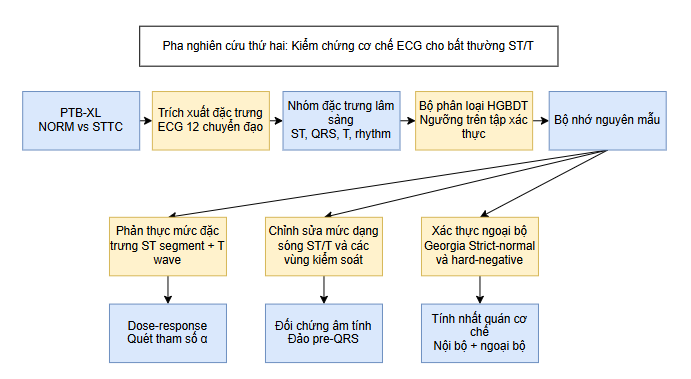
\includegraphics[width=0.98\linewidth]{figure_phase2_pipeline.png}
    \caption{Pipeline tổng thể của pha nghiên cứu thứ hai với các lớp kiểm chứng cơ chế từ mức đặc trưng đến mức dạng sóng và xác thực ngoại bộ.}
    \label{fig:phase2_pipeline}
\end{figure}

\section{Dữ liệu sử dụng}

\blocksep

\subsection{Dữ liệu PTB-XL}

\blocksep

Dữ liệu chính của pha nghiên cứu thứ hai là PTB-XL \cite{Wagner2020} sau khi được chuẩn bị về định dạng CSV 12 chuyển đạo trong nghiên cứu. Theo cách tổ chức của quy trình thực nghiệm, dữ liệu được chia thành ba tập: huấn luyện, xác thực và kiểm tra. Chỉ các mẫu thuộc hai nhóm \texttt{NORM} và \texttt{STTC} mới được sử dụng trong nhiệm vụ chính.

\blocksep

Quy mô dữ liệu cho nhiệm vụ \texttt{NORM vs STTC} gồm 8\,603 mẫu huấn luyện, 1\,116 mẫu xác thực và 1\,082 mẫu kiểm tra, trong đó có 213 mẫu dương tính trong tập kiểm tra.

\blocksep

Trong đó, nhãn 0 tương ứng với nhóm bình thường và nhãn 1 tương ứng với nhóm ST/T bất thường. Cách gán nhãn này được sử dụng nhất quán trong toàn bộ các thí nghiệm chính của pha nghiên cứu thứ hai.

\blocksep

\subsection{Dữ liệu Georgia ngoại bộ}

\blocksep

Để đánh giá mức độ nhất quán của mô hình trên dữ liệu độc lập, nghiên cứu sử dụng thêm bộ dữ liệu Georgia từ PhysioNet Challenge 2020 \cite{Alday2021}. Dữ liệu này được ánh xạ về cùng bài toán ST/T với hai cách chọn mẫu âm tính: \textit{strict\_normal}, chỉ giữ các bản ghi bình thường nghiêm ngặt làm âm tính; và \textit{no\_st\_t}, giữ toàn bộ các bản ghi không mang mã ST/T làm âm tính.

\blocksep

Thiết lập thứ nhất giúp đánh giá trong điều kiện âm tính tương đối “sạch”. Thiết lập thứ hai khó hơn, vì các mẫu âm tính vẫn có thể chứa nhiều bất thường khác ngoài ST/T. Việc sử dụng đồng thời hai cấu hình này giúp tách bạch giữa hiệu năng phân loại và mức độ ổn định của cơ chế tín hiệu khi chuyển miền.

\section{Trích xuất đặc trưng ECG}

\blocksep

\subsection{Nguyên tắc chung}

\blocksep

Trong pha nghiên cứu thứ hai, tín hiệu ECG không được đưa trực tiếp vào một mô hình học sâu đầu-cuối. Thay vào đó, từ mỗi bản ghi ECG 12 chuyển đạo, nghiên cứu trích xuất một vector đặc trưng cố định kích thước. Cách biểu diễn này thuận tiện cho ba mục đích: huấn luyện mô hình phân loại nền, tổ chức đặc trưng theo các nhóm có ý nghĩa lâm sàng và xây dựng phản thực trên từng nhóm đặc trưng.

\blocksep

Theo kết quả tổng hợp, vector đặc trưng cuối cùng có 799 chiều. Đây là đầu vào trực tiếp của mô hình phân loại chính trong các thí nghiệm nội bộ và ngoại bộ.

\blocksep

\subsection{Quy trình trích xuất đặc trưng}

\blocksep

Quá trình trích xuất đặc trưng từ tín hiệu ECG thô bao gồm ba bước chính. Bước đầu tiên là phát hiện đỉnh R. Tín hiệu từ chuyển đạo II được lọc qua bộ lọc thông dải 0.5--40\,Hz để loại nhiễu đường cơ và nhiễu tần số cao, sau đó tính đạo hàm bậc nhất và bình phương để tăng cường độ nhọn của đỉnh. Đỉnh R được xác định bằng thuật toán phát hiện đỉnh cục bộ trên tín hiệu tích phân cửa sổ trượt, với điều kiện khoảng cách tối thiểu tương ứng với 0.25 giây (25 mẫu tại 100\,Hz) và ngưỡng biên độ lấy theo bách phân vị 85 của tín hiệu tích phân. Các đỉnh bất thường với khoảng R-R ngoài dải 0.3--2.0 giây được loại bỏ.

\blocksep

Bước thứ hai là cắt và căn chỉnh nhịp tim. Với mỗi đỉnh R được phát hiện, một cửa sổ cố định gồm \texttt{pre = 80} mẫu trước và \texttt{post = 120} mẫu sau được trích ra, tương ứng tổng cộng 200 mẫu (2 giây tại tần số lấy mẫu 100\,Hz). Trên tất cả 12 chuyển đạo, trung vị cửa sổ qua các đỉnh R được tính để xây dựng \textit{nhịp tim trung vị} đại diện cho bản ghi. Cách lấy trung vị thay vì trung bình giúp giảm ảnh hưởng của các nhịp ngoại lệ hoặc artefact.

\blocksep

Bước thứ ba là trích xuất hai loại đặc trưng từ nhịp tim trung vị. Loại thứ nhất là \textit{thống kê vùng đoạn}: với mỗi vùng sinh lý (P, PR, QRS, ST, T), nghiên cứu tính bốn thống kê cơ bản là giá trị trung bình, độ lệch chuẩn, giá trị nhỏ nhất và lớn nhất trên mỗi trong số 12 chuyển đạo. Loại thứ hai là \textit{điểm hình dạng dạng sóng}: nhịp tim trung vị trên từng chuyển đạo được giảm mẫu xuống 32 điểm để lưu lại hình dạng tổng thể của sóng, độc lập với chiều dài thực tế của bản ghi. Mỗi điểm hình dạng sau đó được gán vào đúng vùng sinh lý tương ứng dựa trên vị trí của nó trong cửa sổ beat, tạo cơ sở cho bước gom nhóm lâm sàng tiếp theo. Toàn bộ đặc trưng được ghép nối trên 12 chuyển đạo, tạo thành vector đặc trưng 799 chiều. Để bảo đảm cùng định dạng trích xuất giữa PTB-XL và Georgia, cả hai bộ dữ liệu đều được lấy mẫu lại về tần số 100\,Hz trước khi đưa vào quy trình trên.

\blocksep

\subsection{Gom đặc trưng theo nhóm lâm sàng}

\blocksep

Một thành phần quan trọng của pha nghiên cứu thứ hai là bước gom đặc trưng. Thay vì xem 799 chiều đặc trưng như một tập không cấu trúc, nghiên cứu chia chúng thành các nhóm tương ứng với các thành phần tín hiệu ECG. Cụ thể, mỗi điểm mẫu dạng sóng trên nhịp tim trung vị (sau khi giảm mẫu xuống 32 điểm mỗi chuyển đạo) được gán vào đúng vùng sinh lý tương ứng dựa trên vị trí của nó trong cửa sổ beat, thay vì gom toàn bộ vào một nhóm chung. Các nhóm chính gồm:

\renewcommand{\labelitemi}{$+$}
\begin{itemize}
	\item \texttt{rhythm} (6 đặc trưng);
	\item \texttt{p\_wave} (91 đặc trưng: 65 thống kê phân đoạn + 26 điểm dạng sóng vùng P);
	\item \texttt{pr\_segment} (65 đặc trưng);
	\item \texttt{qrs} (104 đặc trưng: 65 thống kê + 39 điểm dạng sóng vùng QRS);
	\item \texttt{st\_segment} (104 đặc trưng: 65 thống kê + 39 điểm dạng sóng vùng ST);
	\item \texttt{t\_wave} (143 đặc trưng: 65 thống kê + 78 điểm dạng sóng vùng T);
	\item \texttt{global\_morph} (52 đặc trưng);
	\item \texttt{beat\_baseline} (234 đặc trưng: các điểm dạng sóng thuộc vùng nền trước P và sau T).
\end{itemize}

\blocksep

Trong đó, \texttt{st\_segment} và \texttt{t\_wave} là hai nhóm được quan tâm nhiều nhất trong nhiệm vụ ST/T. Các nhóm sinh lý chính như \texttt{p\_wave}, \texttt{qrs}, \texttt{st\_segment} và \texttt{t\_wave} có kích thước cùng bậc (91--143 đặc trưng), trong khi các nhóm phụ như \texttt{rhythm}, \texttt{global\_morph} và \texttt{beat\_baseline} nhỏ hơn hoặc lớn hơn đáng kể. Cách gom này cho phép xây dựng cả các nhóm đối chứng gần tương đương lẫn các nhóm đối chứng lớn hơn nhóm mục tiêu, nhờ đó việc so sánh hiệu ứng phản thực không phụ thuộc đơn thuần vào số chiều đặc trưng. Các số đặc trưng trên phản ánh 13 kênh tín hiệu đầu vào (không phải 12): sau khi chuẩn bị dữ liệu, file CSV đầu vào gồm 12 cột \texttt{Lead\_*} từ PTB-XL kết hợp với cột \texttt{Voltage} được giữ lại từ nguồn đơn chuyển đạo gốc, đưa tổng số kênh đầu vào lên 13 ($6 + 13 \times 61 = 799$).

\blocksep

Cách gom nhóm này có ý nghĩa thực tế đối với khóa luận. Thay vì diễn giải mức đóng góp của hàng trăm chiều đặc trưng riêng lẻ, người viết có thể thảo luận ở mức gần hơn với trực giác lâm sàng, chẳng hạn như đoạn ST, sóng T, phức bộ QRS hay hình dạng sóng.

\section{Mô hình phân loại nền}

\blocksep

Mô hình chính được sử dụng trong pha nghiên cứu thứ hai là \texttt{HistGradient\discretionary{}{}{}Boosting\discretionary{}{}{}Classifier}. Đây là mô hình nền được dùng trong các thí nghiệm chính và trong báo cáo kết quả cuối cùng của nghiên cứu. Việc lựa chọn mô hình này có ba ưu điểm: xử lý tốt quan hệ phi tuyến giữa các đặc trưng ECG, thời gian huấn luyện và suy luận tương đối gọn, và thuận lợi cho việc xây dựng các phép thử phản thực trên không gian đặc trưng.

\blocksep

Ngưỡng phân loại không được cố định ở 0.5 mà được chọn trên tập xác thực bằng cách tối đa hóa chỉ số Youden. Sau khi xác định ngưỡng, cùng một ngưỡng này được sử dụng cho tập kiểm tra nội bộ và các phép đánh giá ngoại bộ. Điều này giúp việc so sánh kết quả giữa các bước đánh giá nhất quán hơn.

\blocksep

Về mặt công thức, nếu gọi $Se(t)$ là độ nhạy và $Sp(t)$ là độ đặc hiệu tại ngưỡng $t$, thì chỉ số Youden được viết:
\[
J(t) = Se(t) + Sp(t) - 1.
\]
Ngưỡng được chọn là giá trị $t^\star$ làm cực đại $J(t)$ trên tập xác thực.

\blocksep

Trong khóa luận này, hiệu năng phân loại của mô hình chỉ là một phần của đánh giá. Giá trị chính của pha nghiên cứu thứ hai không nằm ở việc huấn luyện một mô hình phân loại ST/T đơn thuần, mà ở việc sử dụng mô hình đó như một nền tảng để kiểm tra cơ chế tín hiệu.

\section{Bộ nhớ nguyên mẫu phản thực}

\blocksep

\subsection{Nguyên tắc xây dựng}

\blocksep

Thành phần đặc trưng nhất của pha nghiên cứu thứ hai là bộ nhớ nguyên mẫu phản thực. Ý tưởng của thành phần này là lưu trữ một số nguyên mẫu đại diện cho từng lớp trong không gian đặc trưng đã chuẩn hóa. Khi cần xây dựng phản thực cho một mẫu dương tính, hệ thống sẽ tìm nguyên mẫu bình thường gần nhất và dùng nguyên mẫu đó như một đích thay thế.

\blocksep

Trong quy trình thực nghiệm, bộ nhớ này được xây dựng bằng cách chuẩn hóa dữ liệu bằng \texttt{StandardScaler}, sau đó gom cụm các mẫu trong từng lớp bằng \texttt{KMeans}. Với mỗi cụm, một mẫu gần tâm cụm nhất được chọn làm mẫu đại diện và được đưa vào bộ nhớ. Nhờ vậy, bộ nhớ không phải lưu toàn bộ dữ liệu huấn luyện nhưng vẫn giữ được các kiểu hình đại diện của từng lớp.

\blocksep

\subsection{Vai trò trong các thí nghiệm phản thực}

\blocksep

Bộ nhớ nguyên mẫu phản thực được sử dụng trong hầu hết các thí nghiệm chính của pha nghiên cứu thứ hai. Với mỗi mẫu dương tính, nghiên cứu tìm nguyên mẫu âm tính gần nhất trong bộ nhớ. Sau đó, các nhóm đặc trưng mục tiêu của mẫu gốc được thay thế dần bằng các giá trị tương ứng từ nguyên mẫu này. Về trực giác, đây là cách xây dựng một phiên bản “gần bình thường hơn” của chính mẫu bệnh, nhưng sự thay đổi chỉ diễn ra trên nhóm đặc trưng đang được kiểm tra.

\blocksep

Cách làm này hợp lý hơn so với việc thay đặc trưng bằng giá trị trung bình toàn cục, vì nguyên mẫu được lấy từ các trường hợp thật trong dữ liệu huấn luyện. Do đó, phản thực tạo ra vẫn gần với phân bố quan sát được trong thực tế hơn.

\section{Phản thực mức đặc trưng}

\blocksep

\subsection{Cách xây dựng phản thực}

\blocksep

Gọi $\mathbf{x}$ là vector đặc trưng của một mẫu dương tính, $\mathbf{p}$ là nguyên mẫu bình thường gần nhất và $G$ là tập cột thuộc nhóm đặc trưng cần can thiệp. Khi đó, phản thực được tạo bằng cách thay các cột trong $G$ của $\mathbf{x}$ bằng giá trị từ $\mathbf{p}$. Trong trường hợp tổng quát, nghiên cứu còn cho phép điều chỉnh cường độ thay thế bằng một hệ số $\alpha \in [0,1]$:
\[
x^{cf}_j =
\begin{cases}
(1-\alpha)x_j + \alpha p_j, & \text{nếu } j \in G,\\
x_j, & \text{nếu } j \notin G.
\end{cases}
\]

\blocksep

Khi $\alpha = 1$, nhóm đặc trưng mục tiêu được thay hoàn toàn. Khi $\alpha$ tăng dần từ 0 đến 1, có thể kiểm tra được quan hệ liều -- đáp ứng của mô hình.

\blocksep

\subsection{Nhóm mục tiêu}

\blocksep

Đối với nhiệm vụ \texttt{NORM vs STTC}, nhóm mục tiêu chính trong các báo cáo cuối là cặp \texttt{st\_segment + t\_wave} (247 đặc trưng). Đây là cặp bao phủ toàn bộ thông tin ST và T ở cả mức thống kê phân đoạn lẫn mức hình dạng sóng. Ngoài ra, nghiên cứu còn thử các nhóm đơn lẻ và các cặp nhóm khác để làm đối chứng.

\blocksep

Ý nghĩa của bước này là xác định xem khi thay đúng nhóm đặc trưng liên quan đến ST/T, xác suất dự đoán dương tính có giảm mạnh hơn các nhóm khác hay không. Vì trong tập đối chứng có cả những nhóm gần tương đương và những nhóm thậm chí lớn hơn nhóm mục tiêu, hiệu ứng vượt trội của nhóm mục tiêu không thể được giải thích đơn thuần bởi sự chênh lệch về số chiều đặc trưng.

\blocksep

\subsection{Các độ đo sử dụng}

\blocksep

Từ phản thực mức đặc trưng, nghiên cứu tính các độ đo sau:

\renewcommand{\labelitemi}{$+$}
\begin{itemize}
	\item \textit{mean probability drop}: mức giảm xác suất trung bình;
	\item \textit{median probability drop}: trung vị mức giảm xác suất;
	\item \textit{flip rate}: tỷ lệ mẫu đổi từ dương sang âm sau phản thực;
	\item \textit{positive drop rate}: tỷ lệ mẫu có xác suất giảm;
	\item \textit{chỉ số nhất quán phản thực}: chênh lệch giữa nhóm mục tiêu và nhóm đối chứng tốt nhất.
\end{itemize}

\blocksep

Các độ đo này được sử dụng nhất quán trong các báo cáo cuối của pha nghiên cứu thứ hai, cả trên PTB-XL nội bộ lẫn trên Georgia ngoại bộ.

\section{Phản thực mức dạng sóng}

\blocksep

\subsection{Động cơ}

\blocksep

Phản thực mức đặc trưng vẫn là phản thực trong không gian biểu diễn. Vì vậy, pha nghiên cứu thứ hai thực hiện thêm một bước kiểm tra mạnh hơn: chỉnh sửa trực tiếp vùng ST/T trên dạng sóng ECG. Sau khi chỉnh sửa, đặc trưng được trích xuất lại từ dạng sóng mới và đưa trở lại vào mô hình.

\blocksep

Nếu mô hình vẫn phản ứng mạnh theo cùng chiều như ở mức đặc trưng, điều đó cho thấy kết luận không chỉ là một hiện tượng của không gian đặc trưng đã trích xuất, mà còn gắn với một thay đổi có ý nghĩa trên tín hiệu gốc.

\blocksep

\subsection{Cửa sổ mục tiêu và cửa sổ đối chứng}

\blocksep

Trong thí nghiệm dạng sóng, cửa sổ mục tiêu là vùng \texttt{ST/T}. Bên cạnh đó, nghiên cứu còn xây dựng các cửa sổ đối chứng như \texttt{pre-QRS}, \texttt{P/PR} và \texttt{QRS}. Các cửa sổ này đóng vai trò đối chứng âm tính.

\blocksep

Nếu mô hình thực sự đang dựa vào vùng ST/T, thì việc chỉnh sửa ST/T phải tạo ra mức giảm xác suất lớn hơn rõ rệt so với việc chỉnh sửa các cửa sổ đối chứng. Đây là nguyên tắc được dùng xuyên suốt trong các thí nghiệm phản thực ở mức dạng sóng.

\blocksep

Nếu gọi $s(t)$ là tín hiệu gốc, $\tilde{s}(t)$ là dạng sóng mục tiêu lấy từ nguyên mẫu bình thường, $W$ là cửa sổ can thiệp và $r(t) \in [0,1]$ là hàm làm trơn ở biên cửa sổ, thì phép chỉnh sửa mức dạng sóng có thể viết khái quát:
\[
s^{cf}(t) =
\begin{cases}
\left(1-\alpha r(t)\right)s(t) + \alpha r(t)\tilde{s}(t), & t \in W,\\
s(t), & t \notin W.
\end{cases}
\]
Viết như vậy cho thấy nghiên cứu không thay toàn bộ tín hiệu ECG, mà chỉ tác động cục bộ lên đúng vùng đang được kiểm tra.

\blocksep

\subsection{Thay đổi dần mức can thiệp và quan hệ liều - đáp ứng}

\blocksep

Một điểm đáng chú ý trong pha nghiên cứu thứ hai là nghiên cứu không chỉ kiểm tra phản thực hoàn toàn, mà còn thực hiện thay đổi dần tham số \(\alpha\). Với các giá trị $\alpha$ tăng dần từ 0 đến 1, mức can thiệp vào vùng ST/T cũng tăng dần. Sau mỗi mức can thiệp, nghiên cứu đo lại xác suất dự đoán và tỷ lệ đổi nhãn.

\blocksep

Nếu mức giảm xác suất và tỷ lệ đổi nhãn tăng dần theo $\alpha$, có thể xem đây là một dạng quan hệ liều -- đáp ứng. Trong ngữ cảnh của khóa luận, đây là một kiểm tra cần thiết để bảo đảm mô hình không chỉ phản ứng với một phép chỉnh sửa đơn lẻ.

\section{Xác thực ngoại bộ}

\blocksep

Sau khi hoàn thành các thí nghiệm trên PTB-XL, nghiên cứu đánh giá lại mô hình trên dữ liệu Georgia. Mục đích của bước này là kiểm tra hai vấn đề riêng biệt: liệu hiệu năng phân loại có còn được duy trì khi chuyển sang dữ liệu ngoài miền huấn luyện hay không, và liệu cơ chế ST/T có còn cho phản ứng phản thực cùng chiều trên dữ liệu ngoại bộ hay không.

\blocksep

Hai câu hỏi trên không hoàn toàn đồng nhất. Một mô hình có thể giảm hiệu năng khi chuyển miền, nhất là dưới thiết lập âm tính khó, nhưng cơ chế phản thực ST/T vẫn giữ được tính nhất quán. Vì vậy, trong pha nghiên cứu thứ hai, phần xác thực ngoại bộ không chỉ nhằm kiểm tra mô hình phân loại, mà còn nhằm kiểm tra cơ chế tín hiệu.

\section{Thiết kế đánh giá}

\blocksep

\subsection{Các độ đo phân loại}

\blocksep

Pha nghiên cứu thứ hai sử dụng các chỉ số phân loại cơ bản: diện tích dưới đường cong ROC, diện tích dưới đường cong precision-recall, độ chính xác cân bằng và F1 vĩ mô.

\blocksep

Các chỉ số này được dùng để mô tả mức phân biệt của mô hình trên dữ liệu nội bộ và ngoại bộ. Tuy nhiên, chúng không phải là cơ sở duy nhất để kết luận về giá trị của phương pháp.

\blocksep

\subsection{Các độ đo cơ chế}

\blocksep

Để đánh giá phần cơ chế, nghiên cứu sử dụng các nhóm độ đo sau:

\renewcommand{\labelitemi}{$+$}
\begin{itemize}
	\item mean probability drop của nhóm mục tiêu;
	\item flip rate của phản thực;
	\item chênh lệch giữa nhóm mục tiêu và nhóm đối chứng tốt nhất;
	\item tính đơn điệu của quá trình thay đổi dần tham số \(\alpha\);
	\item mức độ lặp lại của hiệu ứng trên Georgia ngoại bộ.
\end{itemize}

\blocksep

Những độ đo này được tổng hợp trong các báo cáo kết quả cuối cùng của nghiên cứu.

\blocksep

Trong đó, chỉ số nhất quán phản thực được dùng xuyên suốt trong các báo cáo cuối có thể viết ngắn gọn dưới dạng:
\[
\mathrm{CCS} = \overline{\Delta p}_{\mathrm{target}} - \overline{\Delta p}_{\mathrm{best\ control}},
\]
với $\overline{\Delta p}_{\mathrm{target}}$ là mức giảm xác suất trung bình khi can thiệp lên nhóm mục tiêu, còn $\overline{\Delta p}_{\mathrm{best\ control}}$ là mức giảm xác suất trung bình của nhóm đối chứng không-ST/T mạnh nhất. Giá trị CCS càng lớn thì bằng chứng cho thấy mô hình dựa chọn lọc vào cơ chế ST/T càng mạnh.

\blocksep

\subsection{Ranh giới của kết luận}

\blocksep

Một điểm cần làm rõ trong chương này là ranh giới của kết luận phương pháp. Pha nghiên cứu thứ hai không nhằm chứng minh quan hệ nhân quả sinh lý tuyệt đối giữa ST/T và CAD. Tương tự, pha này cũng không nhằm xây dựng một hệ thống ECG đủ cơ sở để kết luận chẩn đoán CAD chỉ từ một bản ghi điện tâm đồ. Cách diễn giải phù hợp hơn là: mô hình trong pha nghiên cứu thứ hai học được một cơ chế ST/T có thể kiểm tra bằng phản thực, và cơ chế này còn giữ được tính nhất quán ở mức nhất định trên dữ liệu ngoại bộ.

\section{Thảo luận phương pháp}

\blocksep

Ưu điểm chính của cách tiếp cận trong pha nghiên cứu thứ hai là tính cụ thể. Nghiên cứu không cố gắng giải thích một mô hình quá phức tạp bằng các công cụ hậu nghiệm chung chung, mà thiết kế ngay từ đầu một quy trình phù hợp cho việc kiểm tra cơ chế. Việc sử dụng đặc trưng có cấu trúc, gom nhóm theo ý nghĩa lâm sàng và kết hợp với bộ nhớ nguyên mẫu phản thực giúp các thí nghiệm phản thực có thể diễn giải rõ ràng hơn.

\blocksep

Một ưu điểm khác là đánh giá được tổ chức thành nhiều lớp. Ngoài hiệu năng phân loại, nghiên cứu còn kiểm tra phản thực ở mức đặc trưng, phản thực ở mức dạng sóng, đối chứng âm tính và dữ liệu ngoại bộ. Cách đánh giá này chặt chẽ hơn so với việc chỉ báo cáo một vài chỉ số hiệu năng rồi gắn thêm một biểu đồ giải thích.

\blocksep

Tuy nhiên, phương pháp cũng có một số giới hạn. Trước hết, nhãn chính của pha nghiên cứu thứ hai là ST/T bất thường, không phải CAD xác định. Thứ hai, phản thực được xây dựng từ các nguyên mẫu trong không gian đặc trưng nên vẫn phụ thuộc vào cách biểu diễn dữ liệu. Thứ ba, hiệu năng ngoại bộ của mô hình phân loại có thể giảm rõ khi chuyển sang thiết lập âm tính khó. Vì vậy, đóng góp của pha nghiên cứu này nên được hiểu chủ yếu ở mức kiểm chứng cơ chế tín hiệu, không nên mở rộng quá mức sang kết luận triển khai lâm sàng trực tiếp.

\section{Tổng kết chương}

\blocksep

Chương này đã trình bày phương pháp của pha nghiên cứu thứ hai. Trọng tâm của chương là mô tả cách xây dựng mô hình ECG cho nhiệm vụ \texttt{NORM vs STTC}, cách tổ chức đặc trưng theo các nhóm lâm sàng, cơ chế bộ nhớ nguyên mẫu phản thực, cũng như hai lớp phản thực ở mức đặc trưng và mức dạng sóng.

\blocksep

Trên cơ sở đó, pha nghiên cứu thứ hai được định vị như một mô-đun kiểm chứng cơ chế ST/T trên ECG phục vụ bài toán đánh giá CAD trong toàn khóa luận. Giá trị chính của pha này không nằm ở việc thay thế chẩn đoán lâm sàng, mà ở việc cung cấp một cách kiểm tra tương đối cụ thể xem mô hình đang dựa vào cơ chế ST/T đến mức nào. Các kết quả thực nghiệm tương ứng sẽ được trình bày trong Chương~4.

\newpage
\clearpage
\phantomsection

\setcounter{chapter}{3}
\chapter[{THỰC NGHIỆM VÀ ĐÁNH GIÁ}]{Thực nghiệm và đánh giá}

Chương này trình bày các kết quả thực nghiệm của hai pha nghiên cứu đã mô tả trong các chương trước. Nội dung chương được tổ chức thành hai phần tương ứng với hai pha. Trước hết, pha nghiên cứu thứ nhất được đánh giá trên ba bộ dữ liệu lâm sàng dạng bảng nhằm xem xét khả năng phân tầng nguy cơ của \textit{protective score} và độ ổn định của quy trình khai phá luật. Tiếp theo, pha nghiên cứu thứ hai được đánh giá trên dữ liệu ECG 12 chuyển đạo, với trọng tâm là việc kiểm chứng cơ chế ST/T thông qua phản thực mức đặc trưng, phản thực mức dạng sóng, xác thực ngoại bộ và các đối chứng âm tính.

\blocksep

Mục tiêu của chương không chỉ dừng ở việc liệt kê các chỉ số kết quả, mà còn làm rõ ý nghĩa của từng nhóm kết quả đối với phạm vi kết luận của khóa luận. Với pha nghiên cứu thứ nhất, vấn đề chính là liệu \textit{protective score} có thật sự mang giá trị phân tầng nguy cơ CAD hay không. Với pha nghiên cứu thứ hai, câu hỏi trung tâm là liệu mô hình ECG có cho thấy một cơ chế ST/T nhất quán và có thể kiểm tra được hay không.

\section{Thiết lập thực nghiệm}

\blocksep

\subsection{Thiết lập cho pha nghiên cứu thứ nhất}

\blocksep

Pha nghiên cứu thứ nhất được thực hiện trên ba bộ dữ liệu Z-Alizadeh Sani, UCI Cleveland và UCI Hungarian. Toàn bộ quy trình được đánh giá chéo 5 lần theo cơ chế phân tầng. Trong mỗi lần chia dữ liệu, các bước khai phá luật, chọn luật và xây dựng \textit{protective score} chỉ được thực hiện trên tập huấn luyện; tập kiểm tra chỉ được dùng để tính điểm ngoài mẫu và các chỉ số đánh giá cuối cùng.

\blocksep

Các tham số chính của khai phá luật gồm:

\renewcommand{\labelitemi}{$+$}
\begin{itemize}
	\item \texttt{min\_support = 0.06};
	\item \texttt{min\_confidence = 0.60};
	\item \texttt{min\_lift = 1.40};
	\item \texttt{max\_len = 3};
	\item \texttt{top\_n\_rules = 10};
	\item ngưỡng phân tầng \texttt{threshold = 2}.
\end{itemize}

\blocksep

Các độ đo chính của pha này gồm hệ số tương quan hạng Spearman giữa \textit{protective score} và nhãn CAD, tỷ lệ CAD trong hai nhóm điểm cao/thấp, odds ratio giữa hai nhóm, cùng với so sánh mô hình logistic đối chiếu và mô hình logistic có bổ sung \textit{protective score}.

\blocksep

\subsection{Thiết lập cho pha nghiên cứu thứ hai}

\blocksep

Pha nghiên cứu thứ hai được thực hiện trên nhiệm vụ \texttt{NORM vs STTC} của dữ liệu PTB-XL 12 chuyển đạo và được kiểm tra lại trên dữ liệu Georgia ngoại bộ. Mô hình phân loại chính là \texttt{HistGradient\discretionary{}{}{}Boosting\discretionary{}{}{}Classifier}. Trên PTB-XL, số mẫu dùng cho nhiệm vụ chính gồm 8\,603 mẫu huấn luyện, 1\,116 mẫu xác thực và 1\,082 mẫu kiểm tra; trong tập kiểm tra có 213 mẫu dương tính.

\blocksep

Các đặc trưng ECG được chia thành tám nhóm: \texttt{rhythm} (6), \texttt{p\_wave} (91), \texttt{pr\_segment} (65), \texttt{qrs} (104), \texttt{st\_segment} (104), \texttt{t\_wave} (143), \texttt{global\_morph} (52) và \texttt{beat\_baseline} (234). Trên bài toán \texttt{NORM vs STTC}, nhóm mục tiêu chính được sử dụng trong các thí nghiệm phản thực là cặp \texttt{st\_segment + t\_wave} (247 đặc trưng). Mỗi nhóm đặc trưng bao gồm cả thống kê phân đoạn và các điểm dạng sóng tương ứng với đúng vùng sinh lý của nó, cho phép tạo ra các nhóm đối chứng có kích thước gần tương đương hoặc lớn hơn nhóm mục tiêu để so sánh công bằng.

\blocksep

Đối với dữ liệu Georgia, hai cấu hình âm tính được sử dụng: \textit{strict\_normal} (các mẫu bình thường nghiêm ngặt) và \textit{no\_st\_t} (toàn bộ các mẫu không mang mã ST/T).

\blocksep

Các độ đo đánh giá gồm hai nhóm. Nhóm thứ nhất là các chỉ số phân loại quen thuộc như diện tích dưới đường cong ROC, diện tích dưới đường cong precision-recall, độ chính xác cân bằng và F1 vĩ mô. Nhóm thứ hai là các độ đo liên quan đến cơ chế, bao gồm mức giảm xác suất trung bình sau phản thực, tỷ lệ đổi nhãn, chênh lệch giữa nhóm mục tiêu và nhóm đối chứng tốt nhất, tính đơn điệu của quá trình thay đổi dần tham số \(\alpha\), và mức độ lặp lại của hiệu ứng trên dữ liệu ngoại bộ.

\section{Kết quả pha nghiên cứu thứ nhất}

\blocksep

\subsection{Tổng quan kết quả trên ba bộ dữ liệu}

\blocksep

Bảng~\ref{tab:phase1_summary} trình bày các kết quả tổng hợp của pha nghiên cứu thứ nhất trên ba bộ dữ liệu lâm sàng. Có thể thấy \textit{protective score} đều cho tương quan nghịch với nhãn CAD trên cả ba bộ dữ liệu, với hệ số Spearman nằm trong khoảng từ xấp xỉ $-0.49$ đến $-0.61$.

\begin{table}[H]
\centering
\caption{Tổng hợp kết quả chính của pha nghiên cứu thứ nhất}
\label{tab:phase1_summary}
\begin{tabular}{p{0.23\linewidth}C{0.10\linewidth}C{0.13\linewidth}C{0.15\linewidth}C{0.15\linewidth}C{0.10\linewidth}}
\hline
\textbf{Bộ dữ liệu} & \textbf{Số mẫu} & \textbf{$\rho$ Spearman} & \shortstack{\textbf{Tỷ lệ CAD}\\\textbf{điểm cao}} & \shortstack{\textbf{Tỷ lệ CAD}\\\textbf{điểm thấp}} & \textbf{$\Delta$AUC} \\
\hline
Z-Alizadeh & 303 & $-0.613$ & 0.467 & 0.960 & $-0.0004$ \\
UCI Cleveland & 303 & $-0.589$ & 0.184 & 0.759 & $+0.0023$ \\
UCI Hungarian & 294 & $-0.495$ & 0.115 & 0.581 & $+0.0002$ \\
\hline
\end{tabular}
\end{table}

\blocksep

Trên cả ba bộ dữ liệu, nhóm có \textit{protective score} thấp đều có tỷ lệ CAD cao hơn rõ rệt so với nhóm có điểm cao. Kết quả này phù hợp với cách xây dựng điểm: bệnh nhân càng thỏa mãn nhiều dấu hiệu bảo vệ ổn định thì càng có xu hướng thuộc nhóm nguy cơ thấp hơn. Đặc điểm này thể hiện rõ nhất ở bộ Z-Alizadeh, nơi tỷ lệ CAD ở nhóm điểm thấp lên đến khoảng 96.0\%, trong khi ở nhóm điểm cao là khoảng 46.7\%.

\blocksep

\begin{figure}[H]
    \centering
    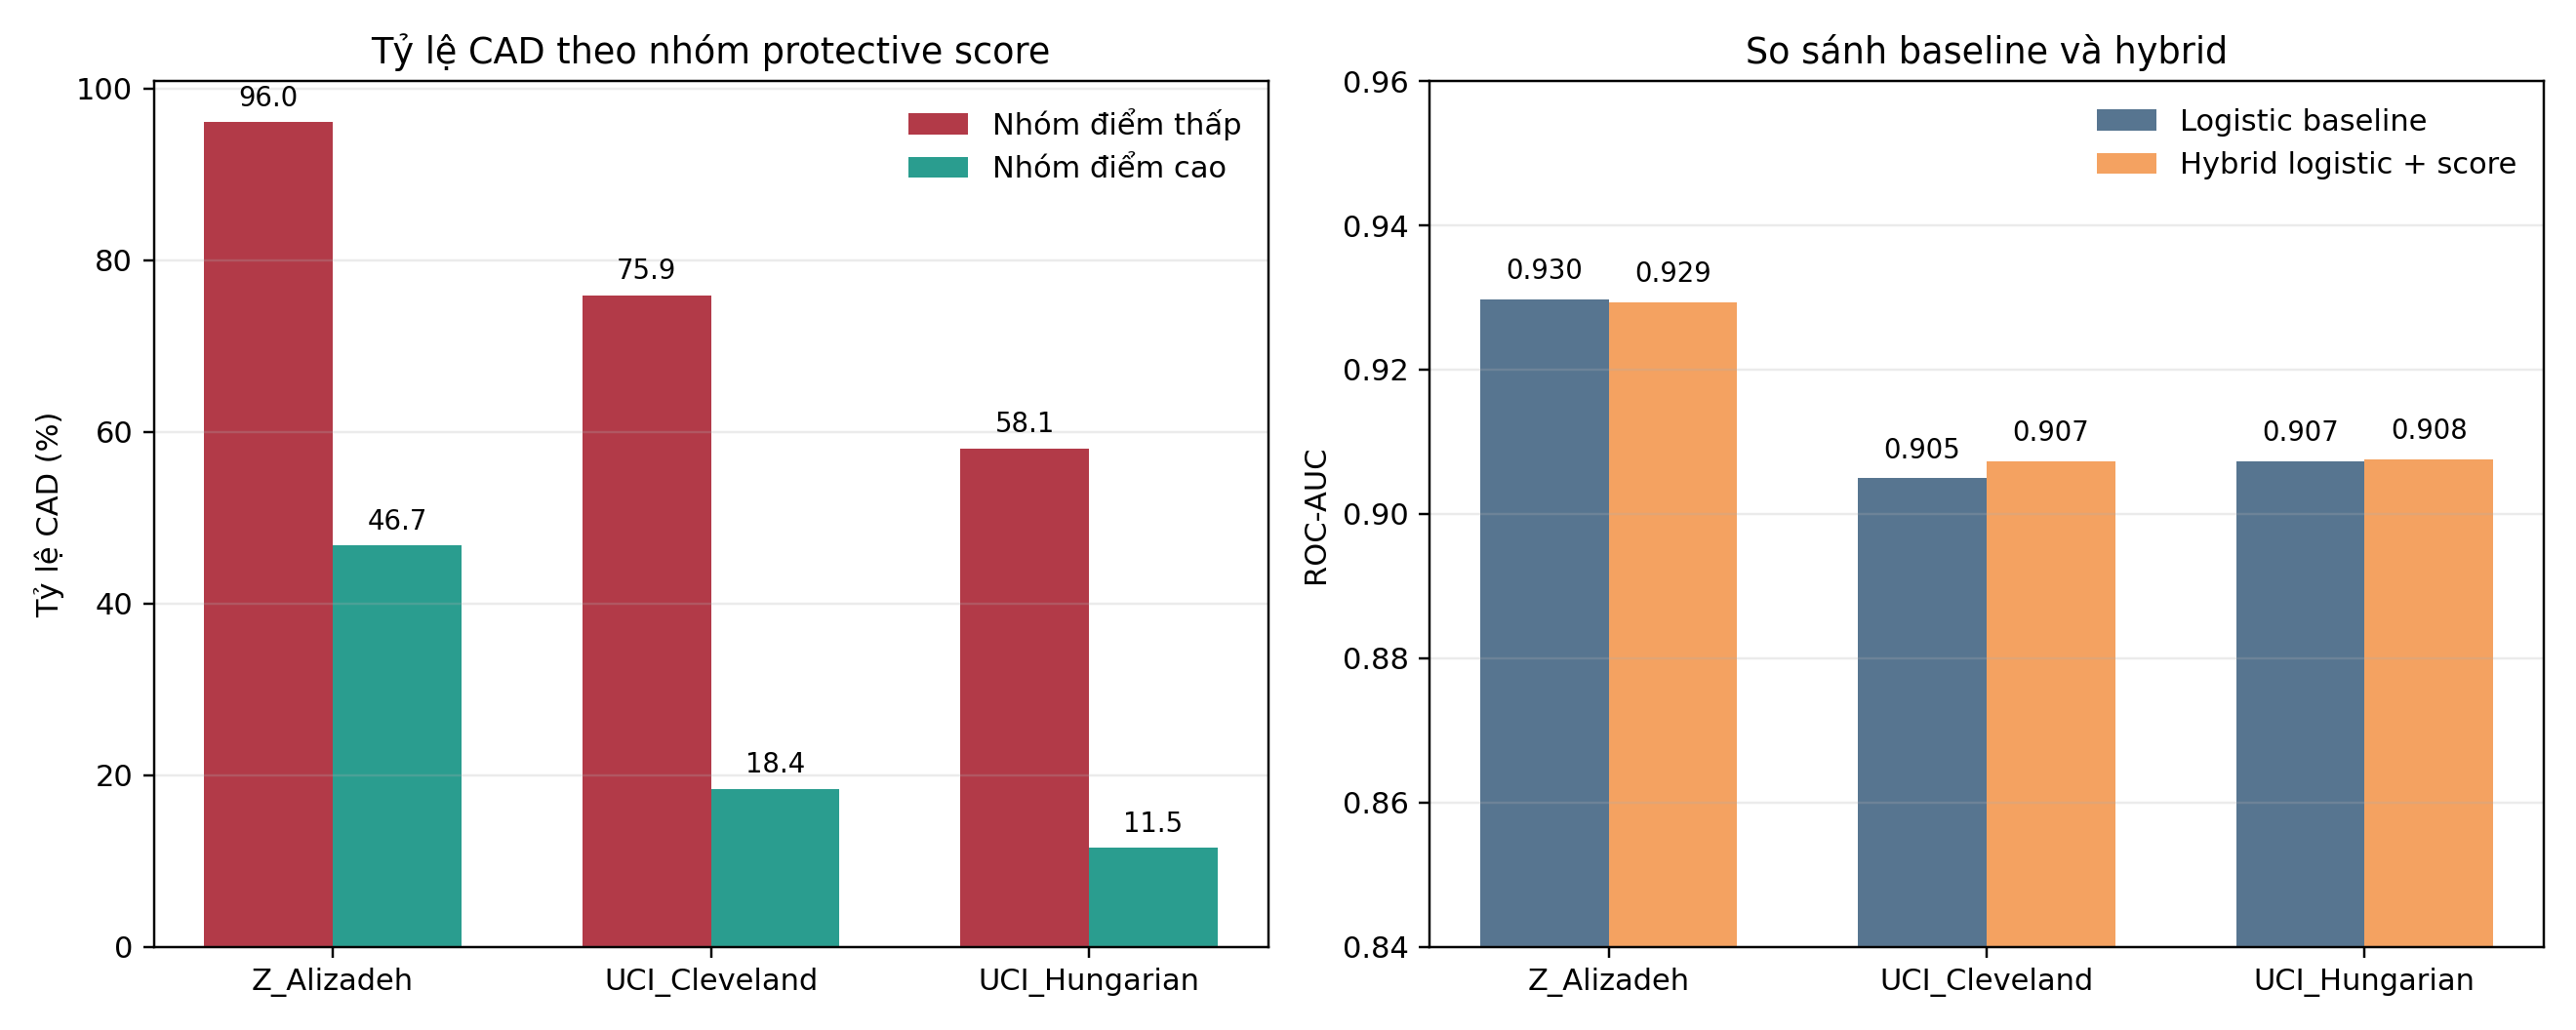
\includegraphics[width=0.95\linewidth]{figure_phase1_summary.png}
    \caption{Tổng hợp kết quả chính của pha nghiên cứu thứ nhất trên ba bộ dữ liệu: tỷ lệ CAD theo nhóm protective score và so sánh hai cấu hình logistic.}
    \label{fig:phase1_summary_result}
\end{figure}

\blocksep

\subsection{Giá trị phân tầng nguy cơ}

\blocksep

Nếu xem xét dưới góc độ phân tầng, kết quả của pha nghiên cứu thứ nhất là khá nhất quán. Trên Z-Alizadeh, odds ratio của nhóm điểm thấp so với nhóm điểm cao xấp xỉ 25.5. Trên UCI Cleveland và UCI Hungarian, giá trị này lần lượt vào khoảng 13.7 và 10.3. Mặc dù các bộ dữ liệu có quy mô nhỏ và cấu trúc biến đầu vào khác nhau, sự tách biệt giữa nhóm điểm cao và nhóm điểm thấp vẫn được duy trì.

\blocksep

Kết quả này cho thấy \textit{protective score} không chỉ mang ý nghĩa trên riêng một bộ dữ liệu. Ngay cả khi số lượng luật và số chiều đặc trưng thay đổi giữa các bộ dữ liệu, cách xây dựng điểm vẫn tạo ra một xu hướng ổn định: điểm càng thấp thì xác suất thuộc nhóm CAD càng cao.

\blocksep

Hình~\ref{fig:phase1_rule_stability_result} cho thấy các tổ hợp luật bảo vệ hàng đầu được lặp lại nhất quán qua các fold của đánh giá chéo. Đây là bằng chứng bổ sung cho thấy giá trị phân tầng nguy cơ của \textit{protective score} không đến từ một vài luật ngẫu nhiên riêng lẻ, mà đến từ các tổ hợp đặc trưng xuất hiện bền vững trên từng bộ dữ liệu.

\blocksep

\begin{figure}[H]
    \centering
    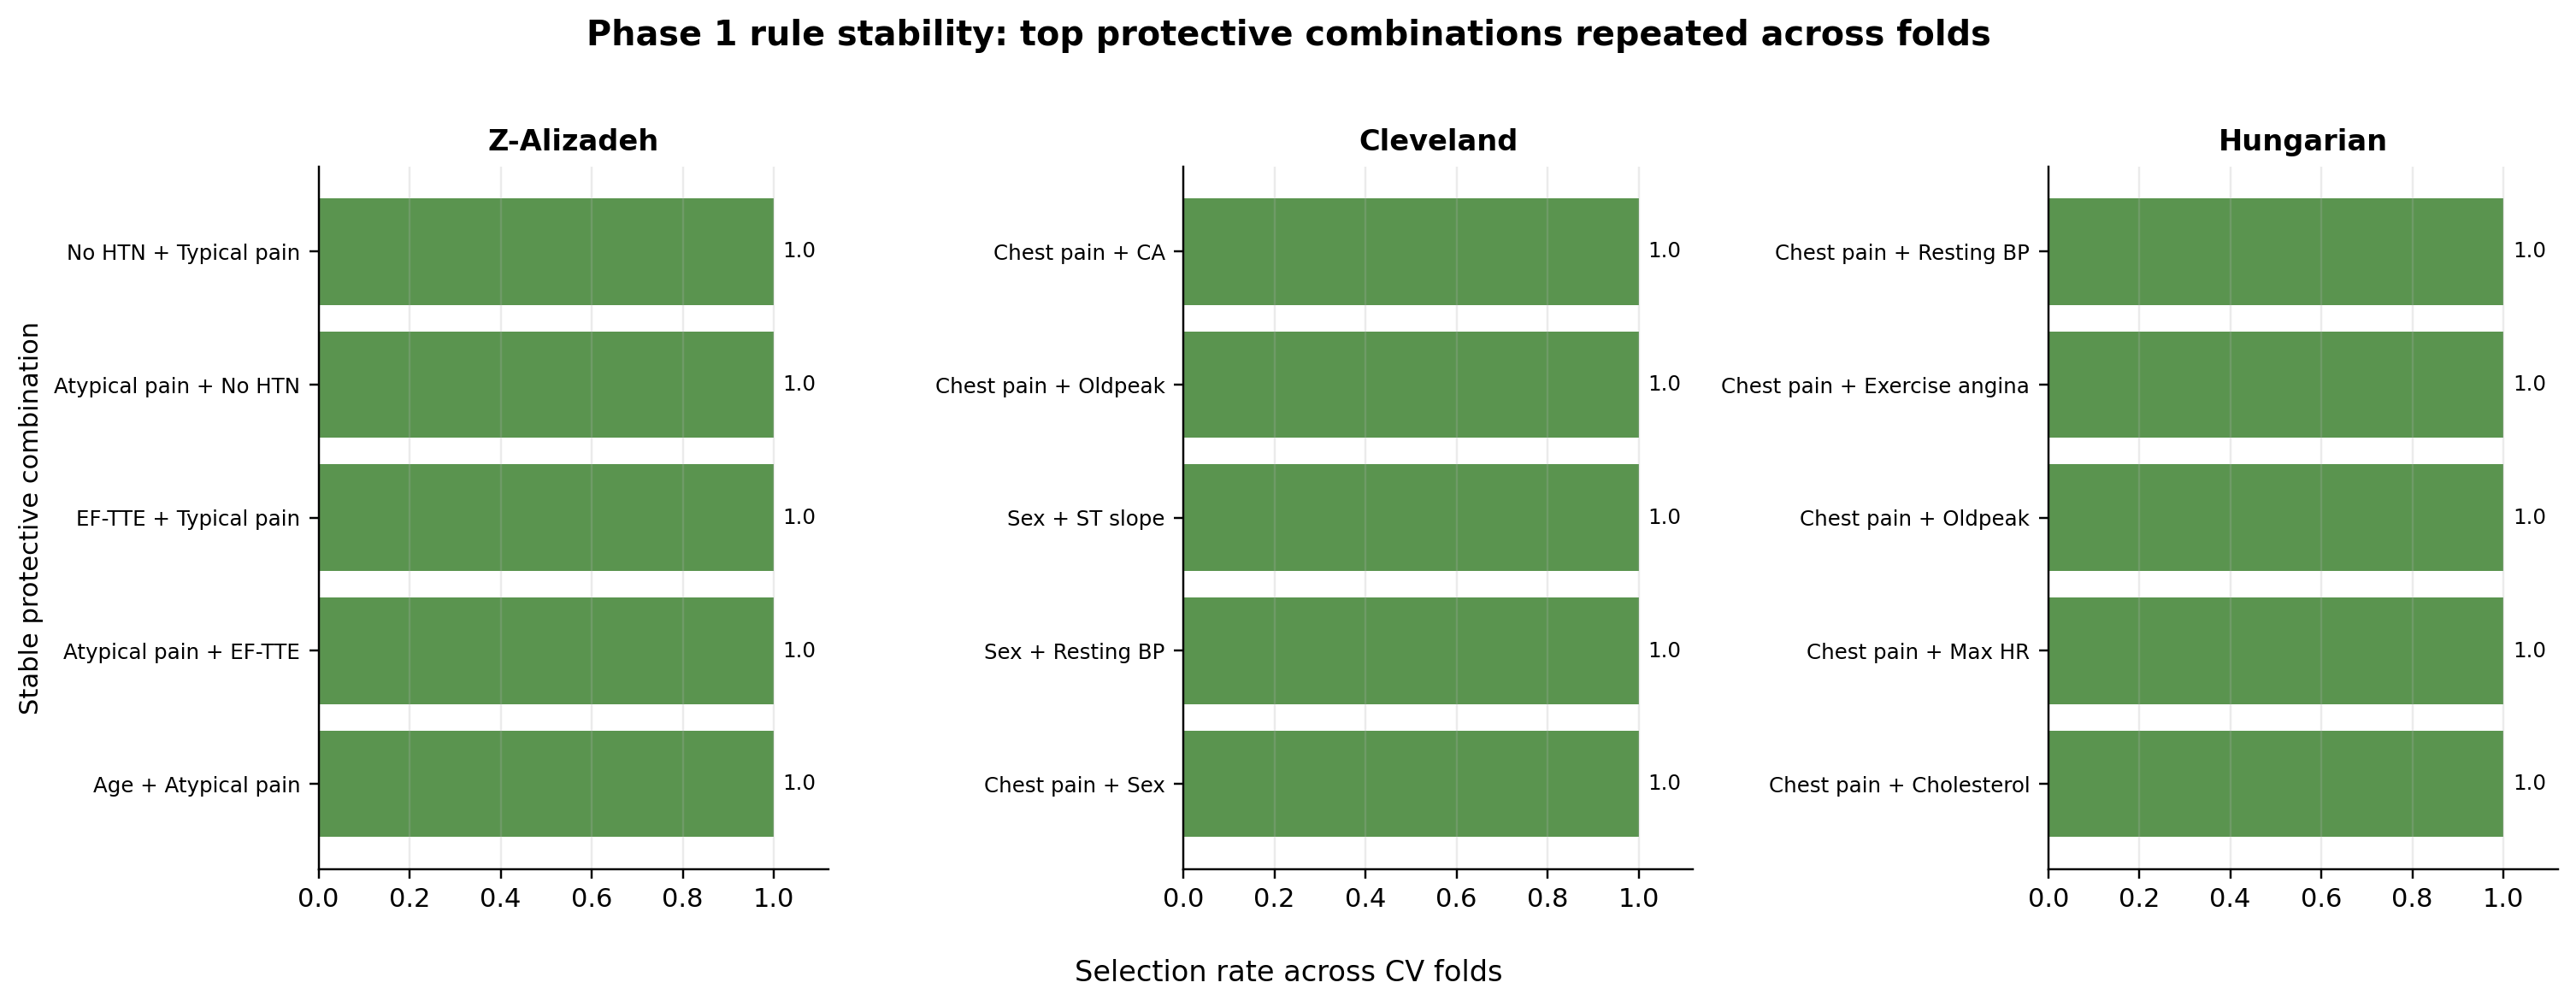
\includegraphics[width=0.98\linewidth]{figure_phase1_rule_stability.png}
    \caption{Độ ổn định của các tổ hợp protective rules hàng đầu qua các fold trên ba bộ dữ liệu của pha nghiên cứu thứ nhất.}
    \label{fig:phase1_rule_stability_result}
\end{figure}

\blocksep

\subsection{So sánh hai cấu hình logistic}

\blocksep

Khi bổ sung \textit{protective score} vào logistic regression, mức thay đổi về diện tích dưới đường cong ROC là rất nhỏ. Trên Z-Alizadeh, AUC của mô hình logistic có bổ sung protective score giảm nhẹ từ 0.9297 xuống 0.9293. Trên UCI Cleveland, AUC tăng từ 0.9049 lên 0.9073. Trên UCI Hungarian, AUC tăng từ 0.9073 lên 0.9075. Các thay đổi này đều có độ lớn rất nhỏ.

\blocksep

Kết quả trên phù hợp với định hướng ban đầu của pha nghiên cứu thứ nhất. \textit{Protective score} không được xây dựng để thay thế hoàn toàn các mô hình phân loại xác suất, cũng không nhằm tối đa hóa AUC. Giá trị chính của phương pháp nằm ở chỗ tạo ra được một lớp tri thức có thể diễn giải và sử dụng cho phân tầng nguy cơ. Vì vậy, phần so sánh giữa mô hình logistic đối chiếu và mô hình logistic có bổ sung \textit{protective score} chỉ nên được xem như một phép kiểm tra phụ trợ, không phải kết quả trung tâm.

\blocksep

Ngoài ra, trên bộ Z-Alizadeh, mối quan hệ giữa \textit{protective score} ngoài mẫu và tỷ lệ CAD cũng được thể hiện trực quan trong Hình~\ref{fig:phase1_zalizadeh_score_result}. Khi điểm tăng, tỷ lệ CAD có xu hướng giảm, phù hợp với cách diễn giải \textit{protective score} như một chỉ số phản ánh mức độ hiện diện của các dấu hiệu bảo vệ.

\blocksep

\begin{figure}[H]
    \centering
    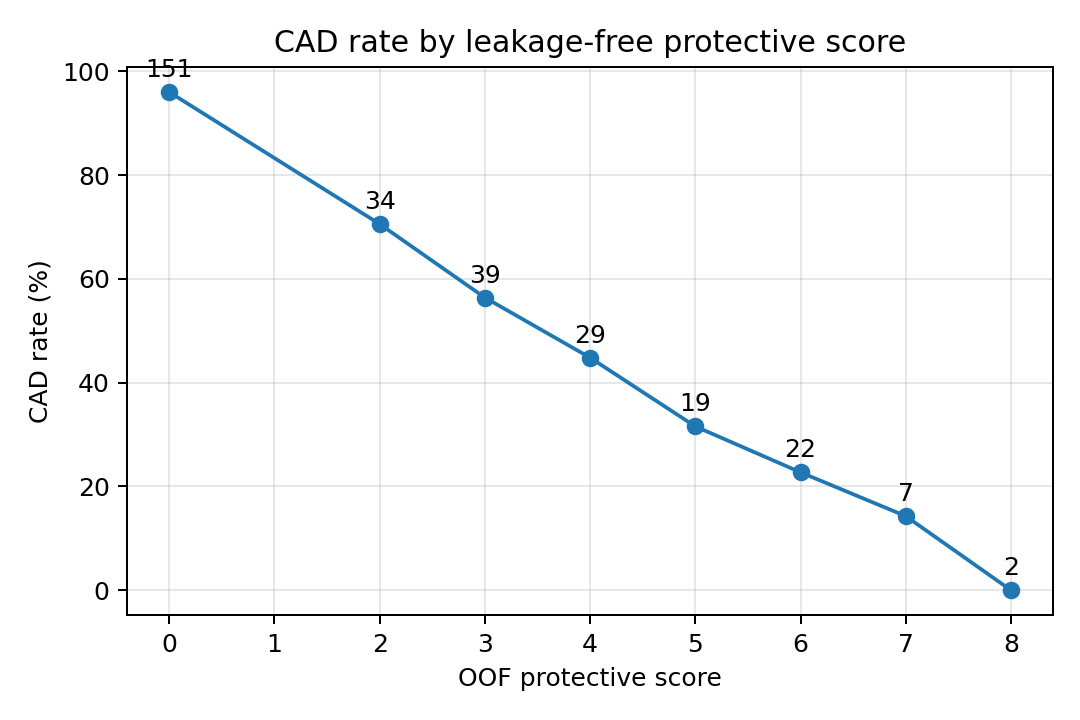
\includegraphics[width=0.78\linewidth]{figure_phase1_zalizadeh_score.png}
    \caption{Ví dụ trên bộ Z-Alizadeh: tỷ lệ CAD theo protective score ngoài mẫu. Con số gắn trên mỗi điểm biểu diễn số lượng mẫu trong mức điểm tương ứng.}
    \label{fig:phase1_zalizadeh_score_result}
\end{figure}

\blocksep

\subsection{Nhận xét chung về pha nghiên cứu thứ nhất}

\blocksep

Nhìn chung, pha nghiên cứu thứ nhất cho thấy hai kết quả đáng chú ý. Thứ nhất, quy trình khai phá luật theo cơ chế ngoài mẫu tạo ra một \textit{protective score} có quan hệ nghịch rõ với nhãn CAD trên cả ba bộ dữ liệu. Thứ hai, phương pháp vẫn giữ được khả năng phân tầng nguy cơ dù số lượng luật và số chiều dữ liệu khác nhau đáng kể giữa các bộ dữ liệu.

\blocksep

Giới hạn của pha này cũng thể hiện khá rõ. Kết quả phụ thuộc vào cách rời rạc hóa biến đầu vào và vào chất lượng biến lâm sàng sẵn có trong từng bộ dữ liệu. Hơn nữa, phương pháp không mang lại một bước nhảy lớn về hiệu năng phân loại xác suất. Vì vậy, đóng góp phù hợp của pha nghiên cứu thứ nhất nên được phát biểu ở mức: xây dựng một lớp phân tầng nguy cơ CAD có thể diễn giải, thay vì một mô hình dự đoán vượt trội về chỉ số phân loại.

\section{Kết quả pha nghiên cứu thứ hai}

\blocksep

\subsection{Hiệu năng phân loại nội bộ trên PTB-XL}

\blocksep

Trên tập kiểm tra nội bộ của nhiệm vụ \texttt{NORM vs STTC}, mô hình nền đạt diện tích dưới đường cong ROC 0.9628, diện tích dưới đường cong precision-recall 0.8973, độ chính xác cân bằng 0.8892 và F1 vĩ mô 0.8308. Các khoảng tin cậy bootstrap 95\% tương đối hẹp, cho thấy hiệu năng của mô hình ổn định trên tập kiểm tra hiện có.

\begin{table}[H]
\centering
\caption{Kết quả phân loại nội bộ trên PTB-XL cho nhiệm vụ \texttt{NORM vs STTC}}
\label{tab:phase2_ptbxl_cls}
\begin{tabular}{p{0.32\linewidth}C{0.18\linewidth}C{0.18\linewidth}C{0.18\linewidth}}
\hline
\textbf{Chỉ số} & \textbf{Giá trị} & \textbf{CI 95\% thấp} & \textbf{CI 95\% cao} \\
\hline
diện tích dưới đường cong ROC & 0.9628 & 0.9502 & 0.9743 \\
diện tích dưới đường cong precision-recall & 0.8973 & 0.8668 & 0.9263 \\
Balanced accuracy & 0.8892 & 0.8676 & 0.9109 \\
Macro-F1 & 0.8308 & 0.8041 & 0.8572 \\
\hline
\end{tabular}
\end{table}

\blocksep

Về mặt phân loại, đây là mức kết quả tốt cho bài toán ST/T trên dữ liệu nội bộ. Tuy nhiên, như đã nêu trong Chương~3, phần đáng quan tâm hơn của pha nghiên cứu này không nằm ở bản thân các chỉ số phân loại, mà ở việc kiểm tra cơ chế ST/T đằng sau dự đoán của mô hình.

\blocksep

\subsection{Phản thực mức đặc trưng trên PTB-XL}

\blocksep

Khi thực hiện phản thực trên cặp nhóm mục tiêu \texttt{st\_segment + t\_wave} (247 đặc trưng), mức giảm xác suất trung bình trên 213 ca dương tính trong tập kiểm tra đạt 0.5240, với khoảng tin cậy 95\% từ 0.4791 đến 0.5692. Tỷ lệ đổi nhãn từ dương sang âm đạt khoảng 43.19\%. Trung vị mức giảm xác suất là 0.5496.

\blocksep

Nhóm đối chứng tốt nhất không thuộc ST/T trong báo cáo này là \texttt{global\_morph + beat\_baseline} (286 đặc trưng), với mức giảm xác suất trung bình chỉ khoảng 0.1400. Điểm đáng chú ý là nhóm đối chứng này có \textit{nhiều đặc trưng hơn} nhóm mục tiêu (286 so với 247), nhưng vẫn cho hiệu ứng yếu hơn rõ rệt. Chênh lệch giữa nhóm mục tiêu và nhóm đối chứng tốt nhất đạt 0.3840 (khoảng tin cậy 95\%: 0.329 đến 0.440). Nếu xét theo tỷ lệ, hiệu ứng của nhóm mục tiêu lớn hơn nhóm đối chứng tốt nhất khoảng 3.74 lần.

\begin{table}[H]
\centering
\caption{Kết quả phản thực mức đặc trưng trên PTB-XL}
\label{tab:phase2_ptbxl_cf}
\begin{tabular}{p{0.35\linewidth}C{0.18\linewidth}C{0.18\linewidth}}
\hline
\textbf{Độ đo} & \textbf{Nhóm mục tiêu} & \textbf{Nhóm đối chứng tốt nhất} \\
\hline
Tổ hợp nhóm & \texttt{st\_segment + t\_wave} & \texttt{global\_morph + beat\_baseline} \\
Số đặc trưng & 247 & 286 \\
Mean probability drop & 0.5240 & 0.1400 \\
Median probability drop & 0.5496 & 0.0364 \\
Flip rate & 0.4319 & 0.1080 \\
Positive drop rate & 0.9577 & 0.8685 \\
\hline
\end{tabular}
\end{table}

\blocksep

Kết quả này cho thấy khi thay đúng nhóm đặc trưng liên quan đến ST/T bằng nguyên mẫu bình thường, dự đoán của mô hình thay đổi mạnh hơn rõ rệt so với các nhóm không-ST/T. Việc nhóm đối chứng tốt nhất có nhiều đặc trưng hơn nhóm mục tiêu nhưng vẫn cho hiệu ứng yếu hơn là một bằng chứng quan trọng: khác biệt quan sát được không thể quy đơn thuần về kích thước nhóm, mà phản ánh vai trò thực chất của nội dung sinh lý thuộc vùng ST/T.

\blocksep

Hình~\ref{fig:phase2_cf_comparison} tổng hợp trực quan kết quả so sánh tất cả các nhóm đặc trưng.

\blocksep

\begin{figure}[H]
    \centering
    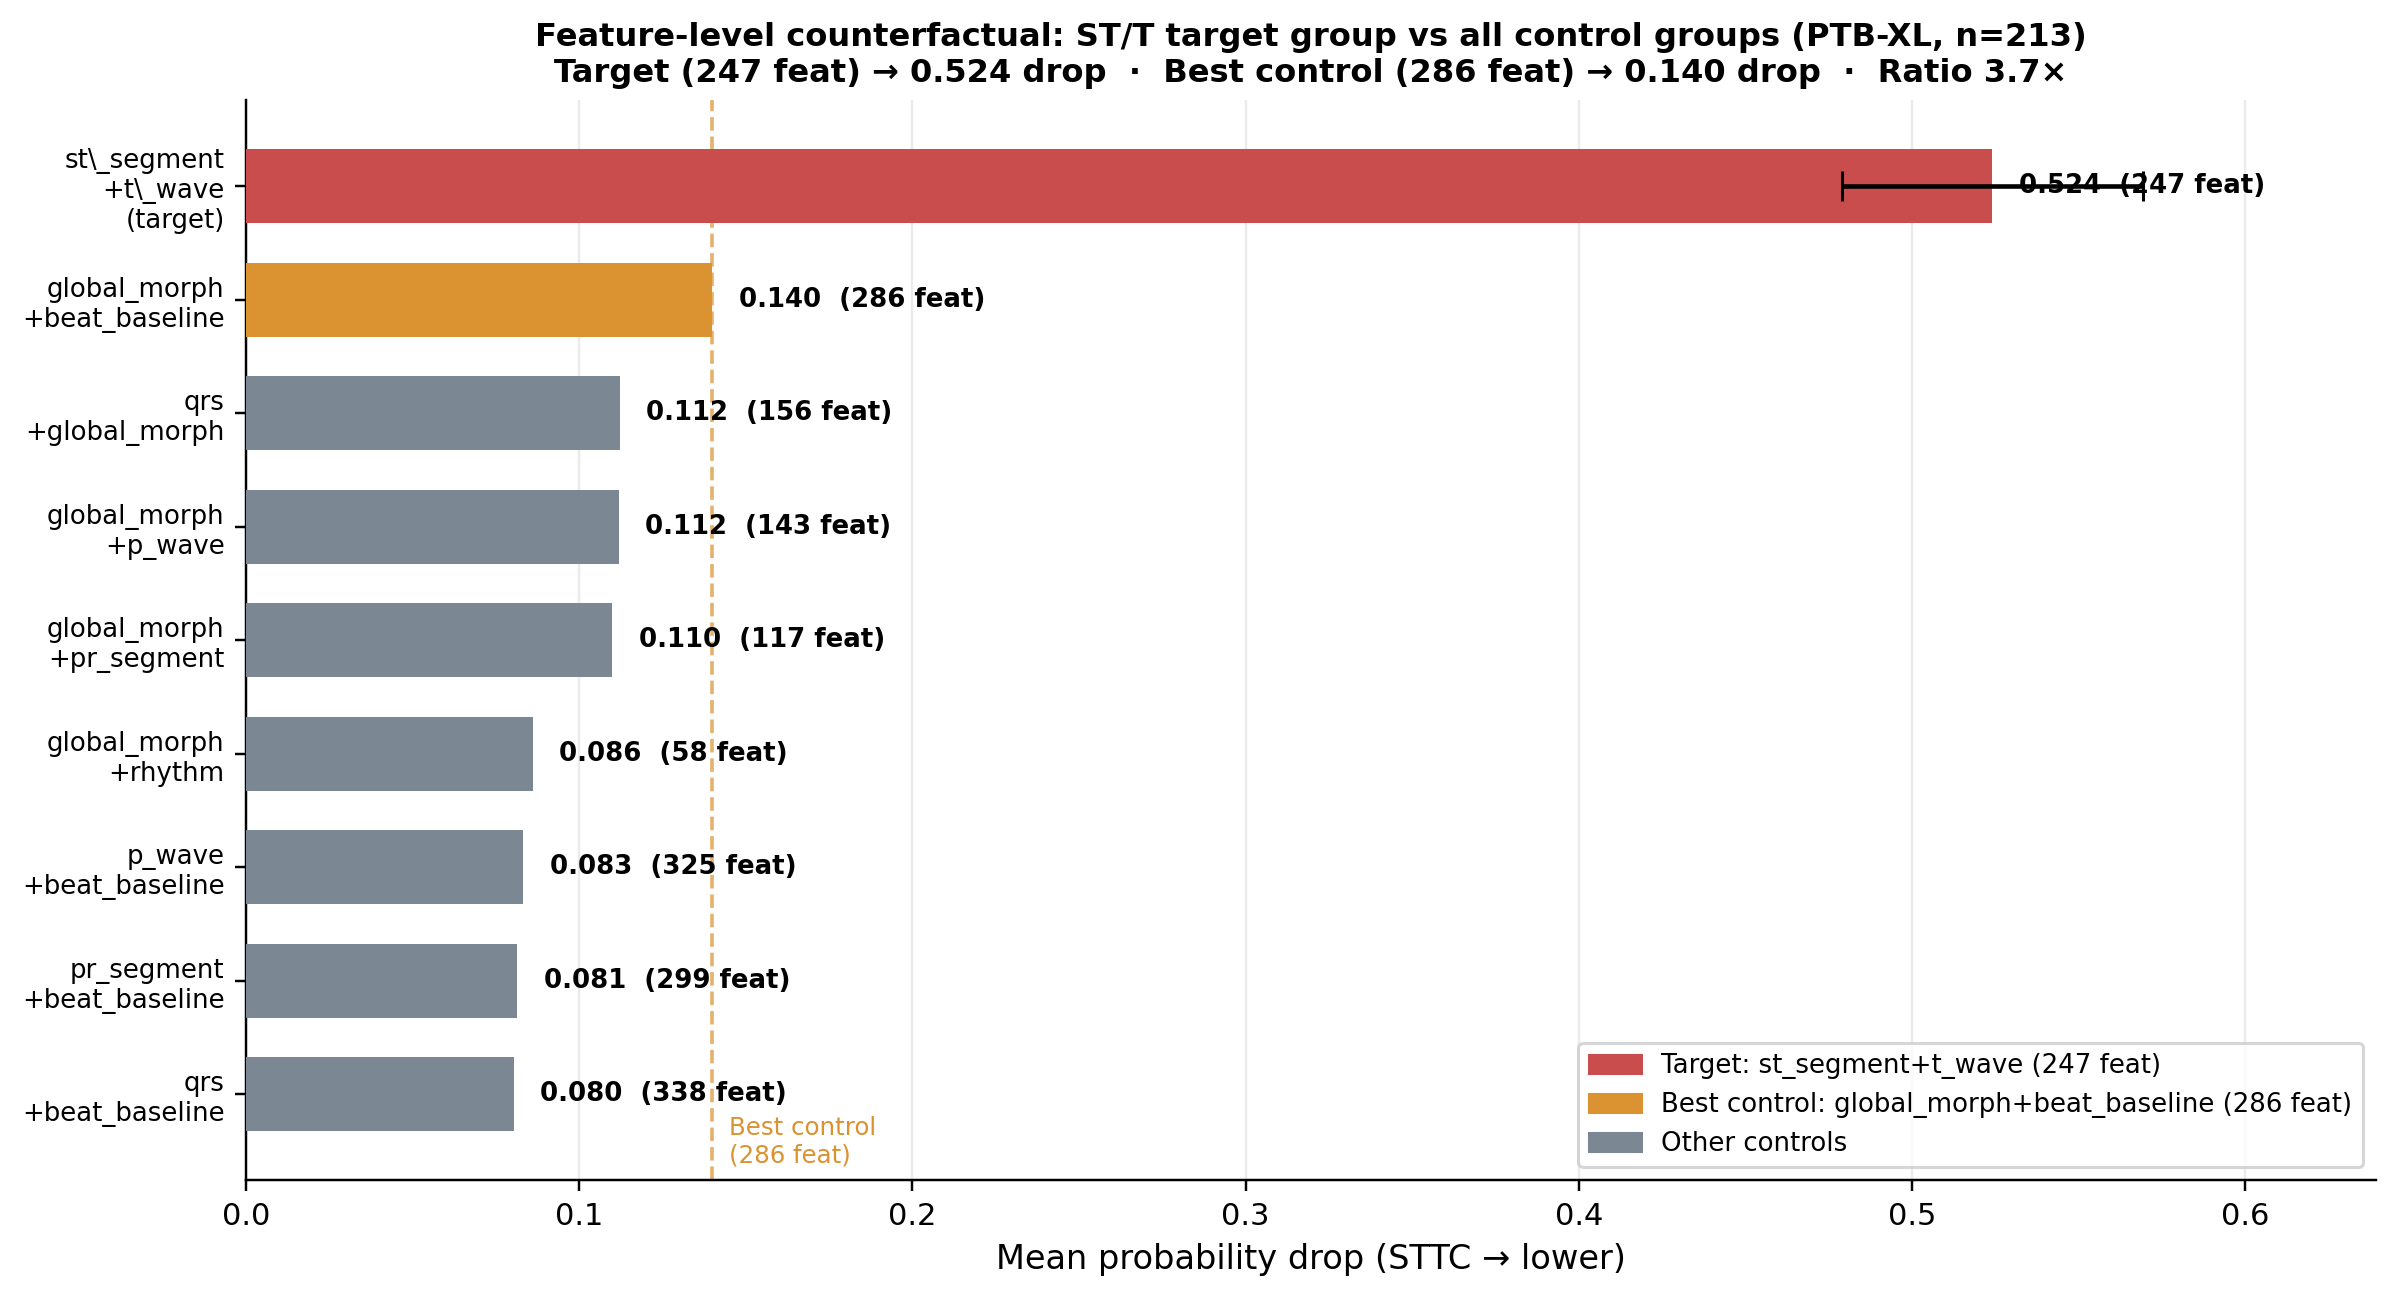
\includegraphics[width=\linewidth, height=9cm, keepaspectratio]{figure_phase2_cf_comparison.png}
    \caption{So sánh hiệu ứng phản thực giữa nhóm mục tiêu \texttt{st\_segment + t\_wave} (247 đặc trưng) và tất cả các nhóm đối chứng trên PTB-XL. Nhóm đối chứng tốt nhất \texttt{global\_morph + beat\_baseline} có 286 đặc trưng, lớn hơn nhóm mục tiêu, nhưng vẫn cho mức giảm thấp hơn rõ rệt.}
    \label{fig:phase2_cf_comparison}
\end{figure}

\blocksep

\subsection{Phản thực mức dạng sóng trên PTB-XL}

\blocksep

Phản thực mức dạng sóng tiếp tục kiểm tra cùng giả thuyết ở mức tín hiệu gốc. Khi chỉnh sửa trực tiếp vùng ST/T trên dạng sóng, mức giảm xác suất trung bình đạt 0.5817, với khoảng tin cậy 95\% từ 0.5326 đến 0.6318. Trung vị mức giảm xác suất là 0.6847. Tỷ lệ đổi nhãn là khoảng 48.36\%, còn tỷ lệ mẫu có xác suất giảm là khoảng 92.49\%.

\blocksep

Trong cùng báo cáo, cửa sổ đối chứng tốt nhất trên PTB-XL là \texttt{P/PR}, chỉ cho mức giảm trung bình khoảng 0.0254; cửa sổ \texttt{QRS} cũng gần tương đương với mức giảm khoảng 0.0252. Đáng chú ý hơn, cửa sổ \texttt{pre-QRS} cho mức giảm trung bình âm, khoảng $-0.0838$. Điều này cho thấy khi chỉnh sửa ở vùng \texttt{pre-QRS}, mô hình không những không giảm xác suất theo cùng chiều, mà còn có xu hướng phản ứng ngược lại.

\blocksep

Nếu so sánh trực tiếp, chênh lệch giữa cửa sổ mục tiêu ST/T và cửa sổ \texttt{pre-QRS} đạt khoảng 0.6656. Đây là đối chứng âm tính mạnh nhất ở mức dạng sóng trong pha nghiên cứu thứ hai. Lý do là \texttt{pre-QRS} nằm ngoài vùng ST/T mục tiêu; do đó, nếu mô hình chỉ phản ứng với việc “chỉnh sửa bất kỳ” trên tín hiệu, hiệu ứng ở cửa sổ này phải cùng chiều hoặc ít nhất không quá khác biệt. Kết quả ngược lại cho thấy mô hình không phản ứng một cách không chọn lọc với mọi can thiệp trên dạng sóng, mà phản ứng chủ yếu khi tác động đúng vào vùng ST/T.

\blocksep

Hình~\ref{fig:phase2_waveform_controls} tổng hợp trực quan các cửa sổ mục tiêu và cửa sổ đối chứng ở mức dạng sóng trên cả PTB-XL và Georgia. Có thể thấy hiệu ứng lớn nhất luôn thuộc về cửa sổ \texttt{ST/T}, trong khi các cửa sổ \texttt{QRS}, \texttt{P/PR} và đặc biệt \texttt{pre-QRS} cho hiệu ứng nhỏ hơn nhiều hoặc đảo dấu.

\blocksep

\begin{figure}[H]
    \centering
    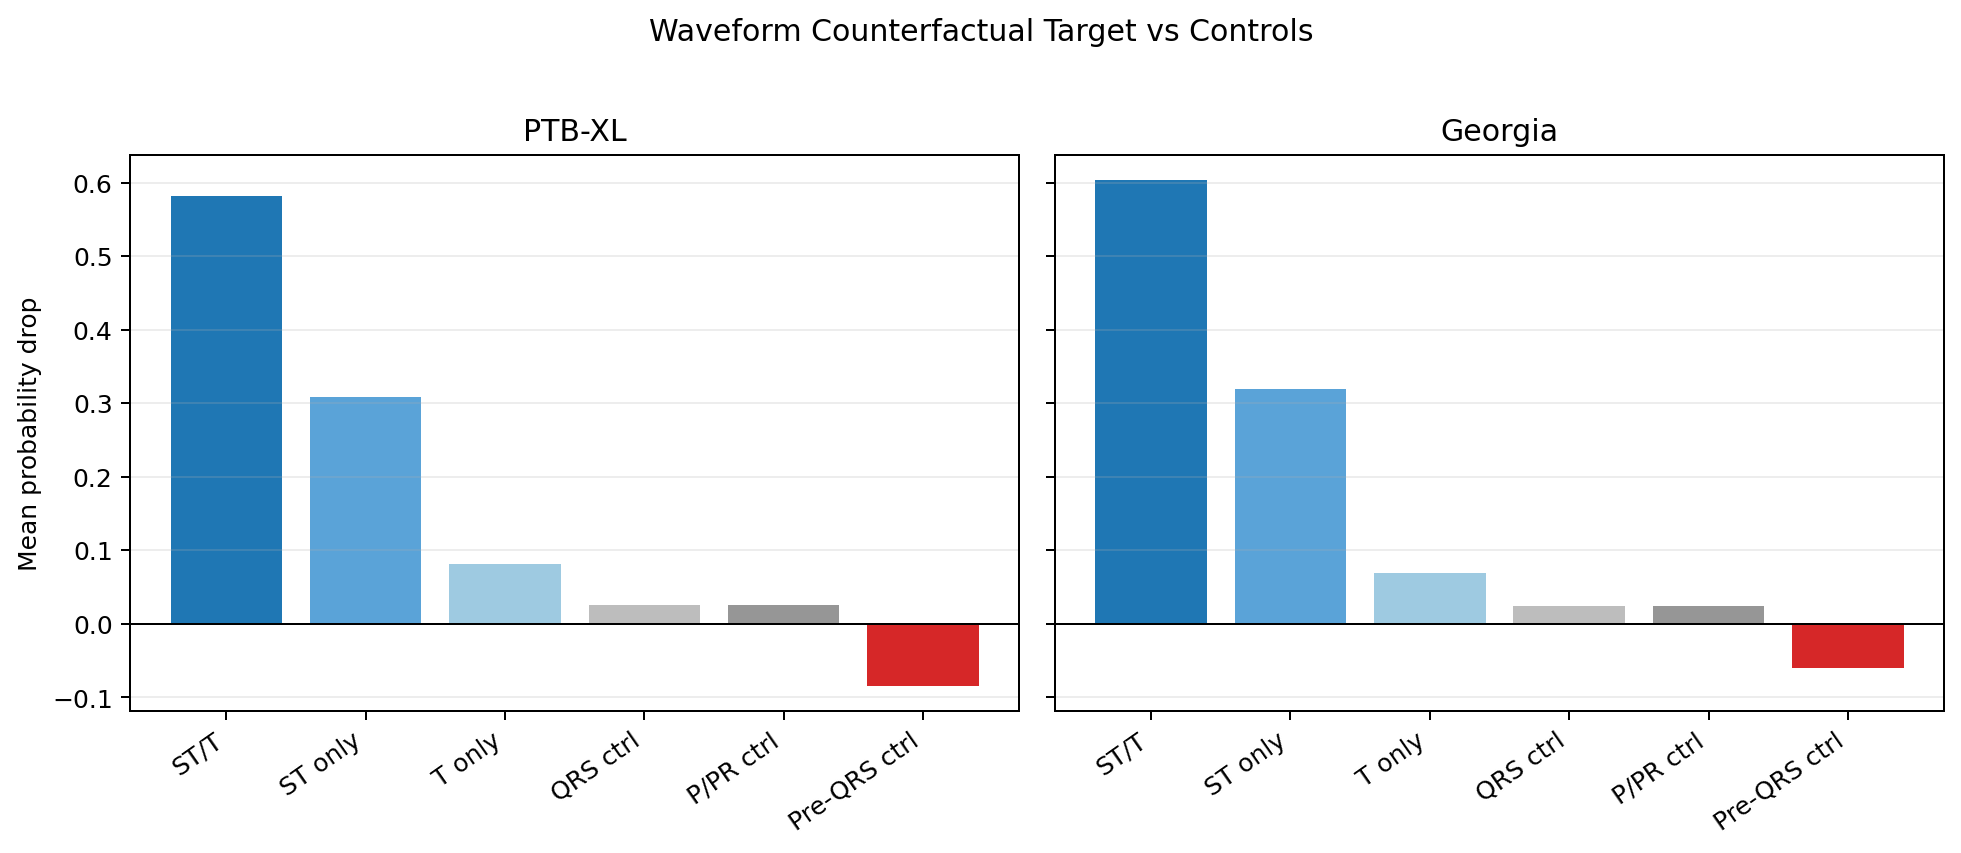
\includegraphics[width=0.95\linewidth]{figure_waveform_controls.png}
    \caption{So sánh mức giảm xác suất giữa cửa sổ mục tiêu ST/T và các cửa sổ đối chứng ở mức dạng sóng trên PTB-XL và Georgia.}
    \label{fig:phase2_waveform_controls}
\end{figure}

\blocksep

\begin{figure}[H]
    \centering
    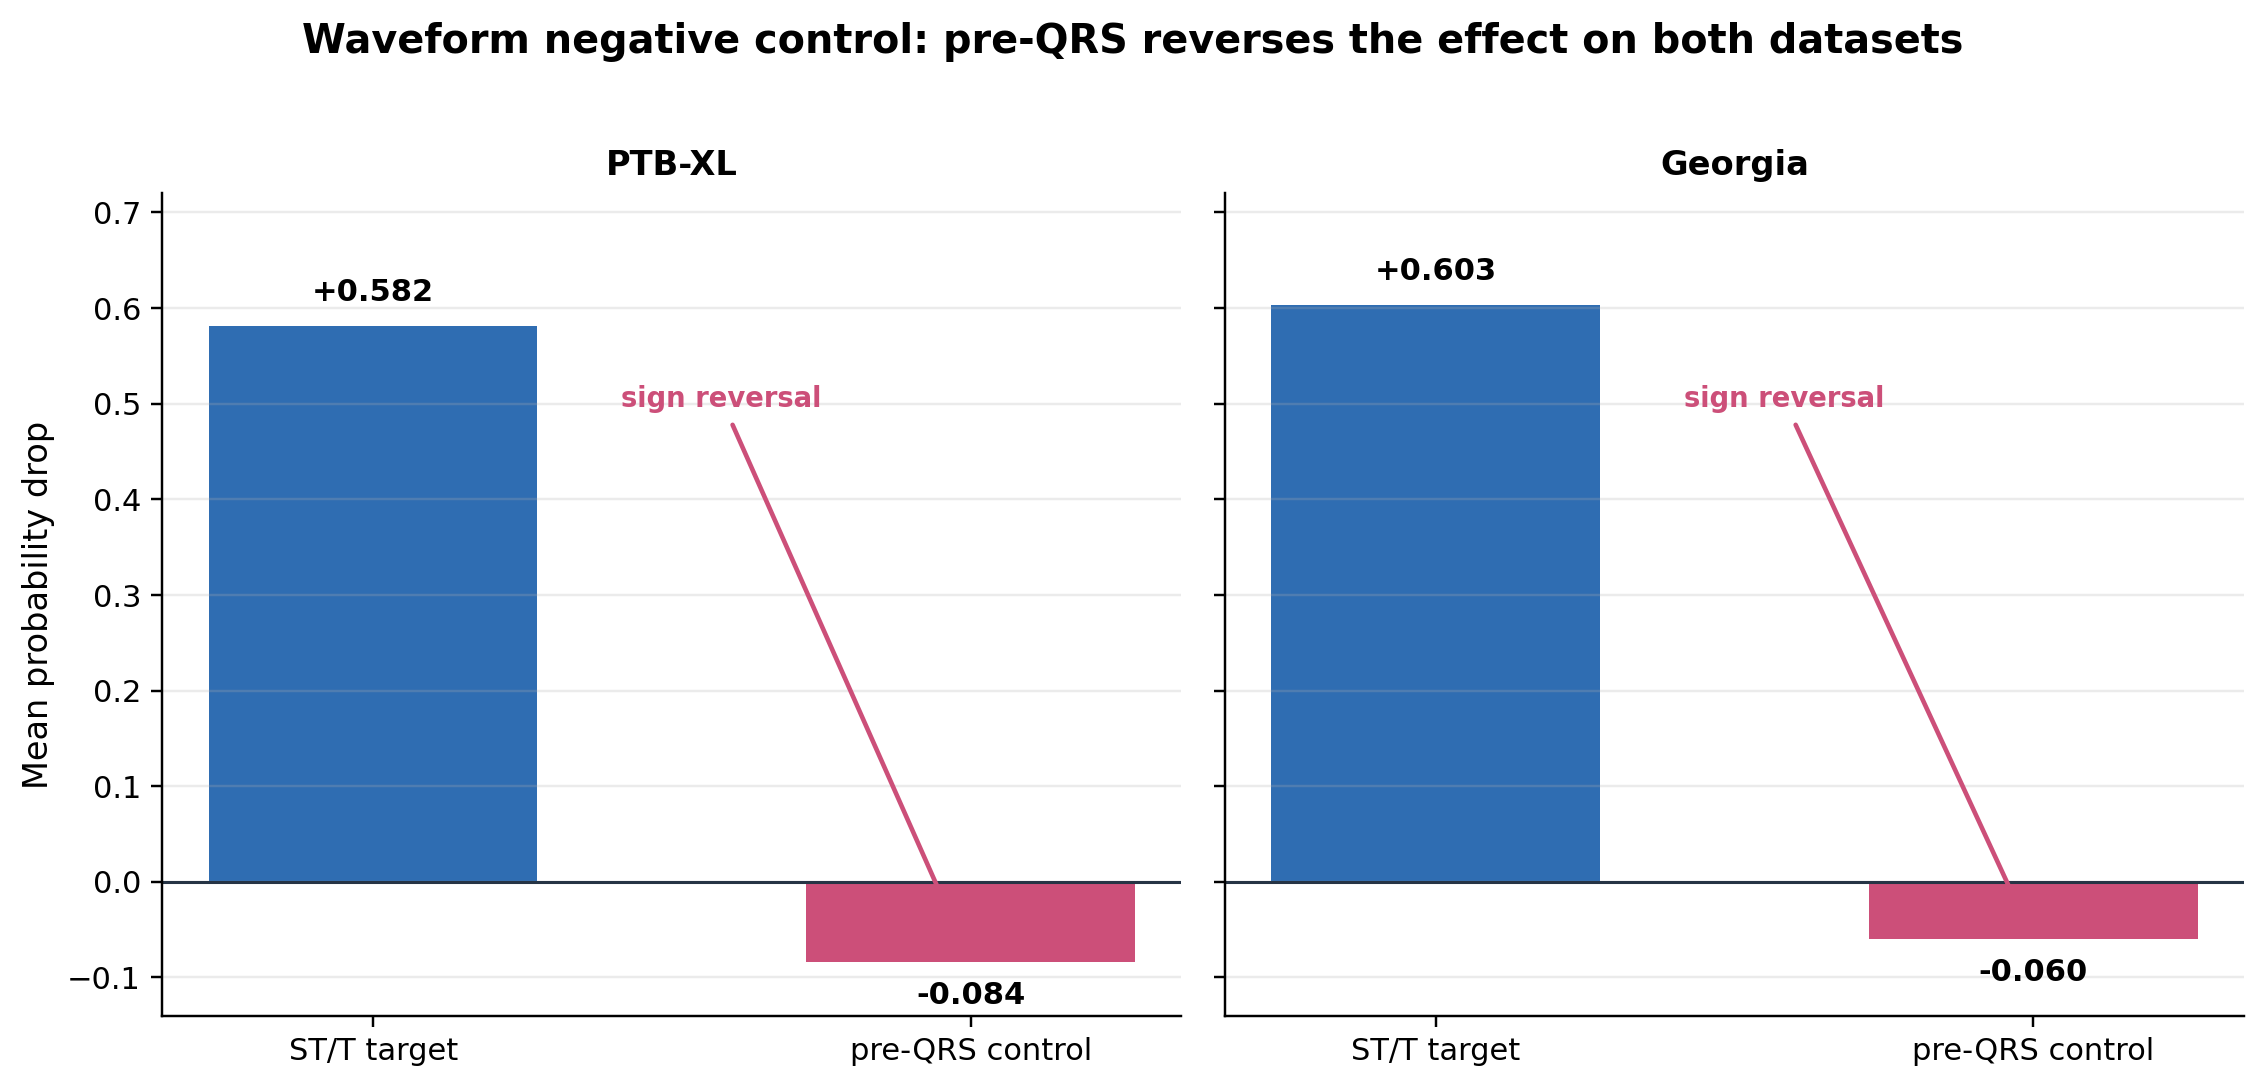
\includegraphics[width=0.95\linewidth]{figure_phase2_preqrs_negative_control.png}
    \caption{Đối chứng âm tính \texttt{pre-QRS} cho hiệu ứng đảo dấu trên cả PTB-XL và Georgia, cho thấy mô hình không phản ứng đồng đều với mọi thao tác chỉnh sửa dạng sóng.}
    \label{fig:phase2_preqrs_negative_control}
\end{figure}

\subsection{Quan hệ liều -- đáp ứng trên PTB-XL}

\blocksep

Thí nghiệm thay đổi dần tham số \(\alpha\) cho thấy mức giảm xác suất tăng dần theo cường độ chỉnh sửa ST/T. Cụ thể, trên PTB-XL, mức giảm xác suất trung bình lần lượt là 0.1264, 0.3072, 0.4890 và 0.5817 tương ứng với $\alpha = 0.25$, $0.50$, $0.75$ và $1.00$.

\blocksep

Xu hướng tăng gần đơn điệu này là một kết quả quan trọng. Nó cho thấy mô hình không chỉ phản ứng với một phép thay thế hoàn toàn, mà còn phản ứng tương ứng với mức độ “bình thường hóa” của vùng ST/T. Trong ngữ cảnh của khóa luận, đây là một kiểm tra cần thiết để tránh việc kết luận cơ chế chỉ dựa trên một thao tác chỉnh sửa đơn lẻ.

\blocksep

\begin{figure}[H]
    \centering
    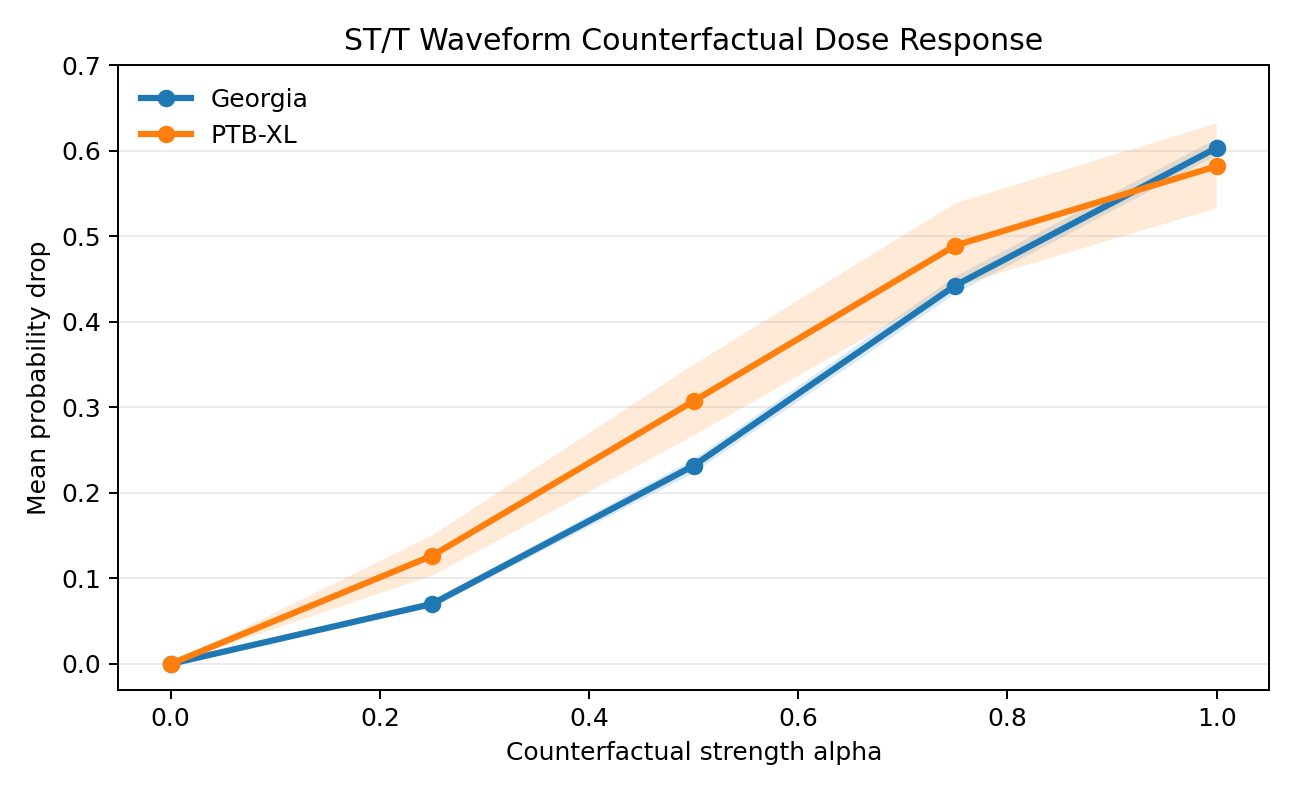
\includegraphics[width=0.88\linewidth]{figure_waveform_dose_response.png}
    \caption{Quan hệ liều -- đáp ứng của phản thực dạng sóng ST/T trên PTB-XL và Georgia khi tăng dần cường độ can thiệp $\alpha$.}
    \label{fig:phase2_waveform_dose_response}
\end{figure}

\subsection{Xác thực ngoại bộ trên Georgia}

\blocksep

Trên dữ liệu Georgia với cấu hình \textit{strict\_normal}, mô hình đạt diện tích dưới đường cong ROC 0.9088, diện tích dưới đường cong precision-recall 0.9600 và độ chính xác cân bằng 0.7896. Khi chuyển sang cấu hình âm tính khó hơn \textit{no\_st\_t}, diện tích dưới đường cong ROC giảm còn 0.8228, diện tích dưới đường cong precision-recall còn 0.7667 và độ chính xác cân bằng còn 0.6900.

\begin{table}[H]
\centering
\caption{Kết quả phân loại ngoại bộ trên Georgia}
\label{tab:phase2_georgia_cls}
\begin{tabular}{p{0.28\linewidth}C{0.14\linewidth}C{0.14\linewidth}C{0.18\linewidth}C{0.14\linewidth}}
\hline
\textbf{Cấu hình} & \textbf{Số mẫu} & \textbf{diện tích dưới đường cong ROC} & \textbf{diện tích dưới đường cong precision-recall} & \textbf{Balanced accuracy} \\
\hline
\textit{strict\_normal} & 6\,341 & 0.9088 & 0.9600 & 0.7896 \\
\textit{no\_st\_t} & 10\,327 & 0.8228 & 0.7667 & 0.6900 \\
\hline
\end{tabular}
\end{table}

\blocksep

Hình~\ref{fig:phase2_external_validation} trực quan hóa mức suy giảm hiệu năng khi chuyển từ kiểm tra nội bộ PTB-XL sang hai cấu hình ngoại bộ Georgia. Kết quả này được trình bày trong phần chính vì nó giúp làm rõ ranh giới của mô hình nền: hiệu năng phân loại vẫn hữu ích trên Georgia, nhưng suy giảm rõ khi nhóm âm tính trở nên khó hơn.

\blocksep

\begin{figure}[H]
    \centering
    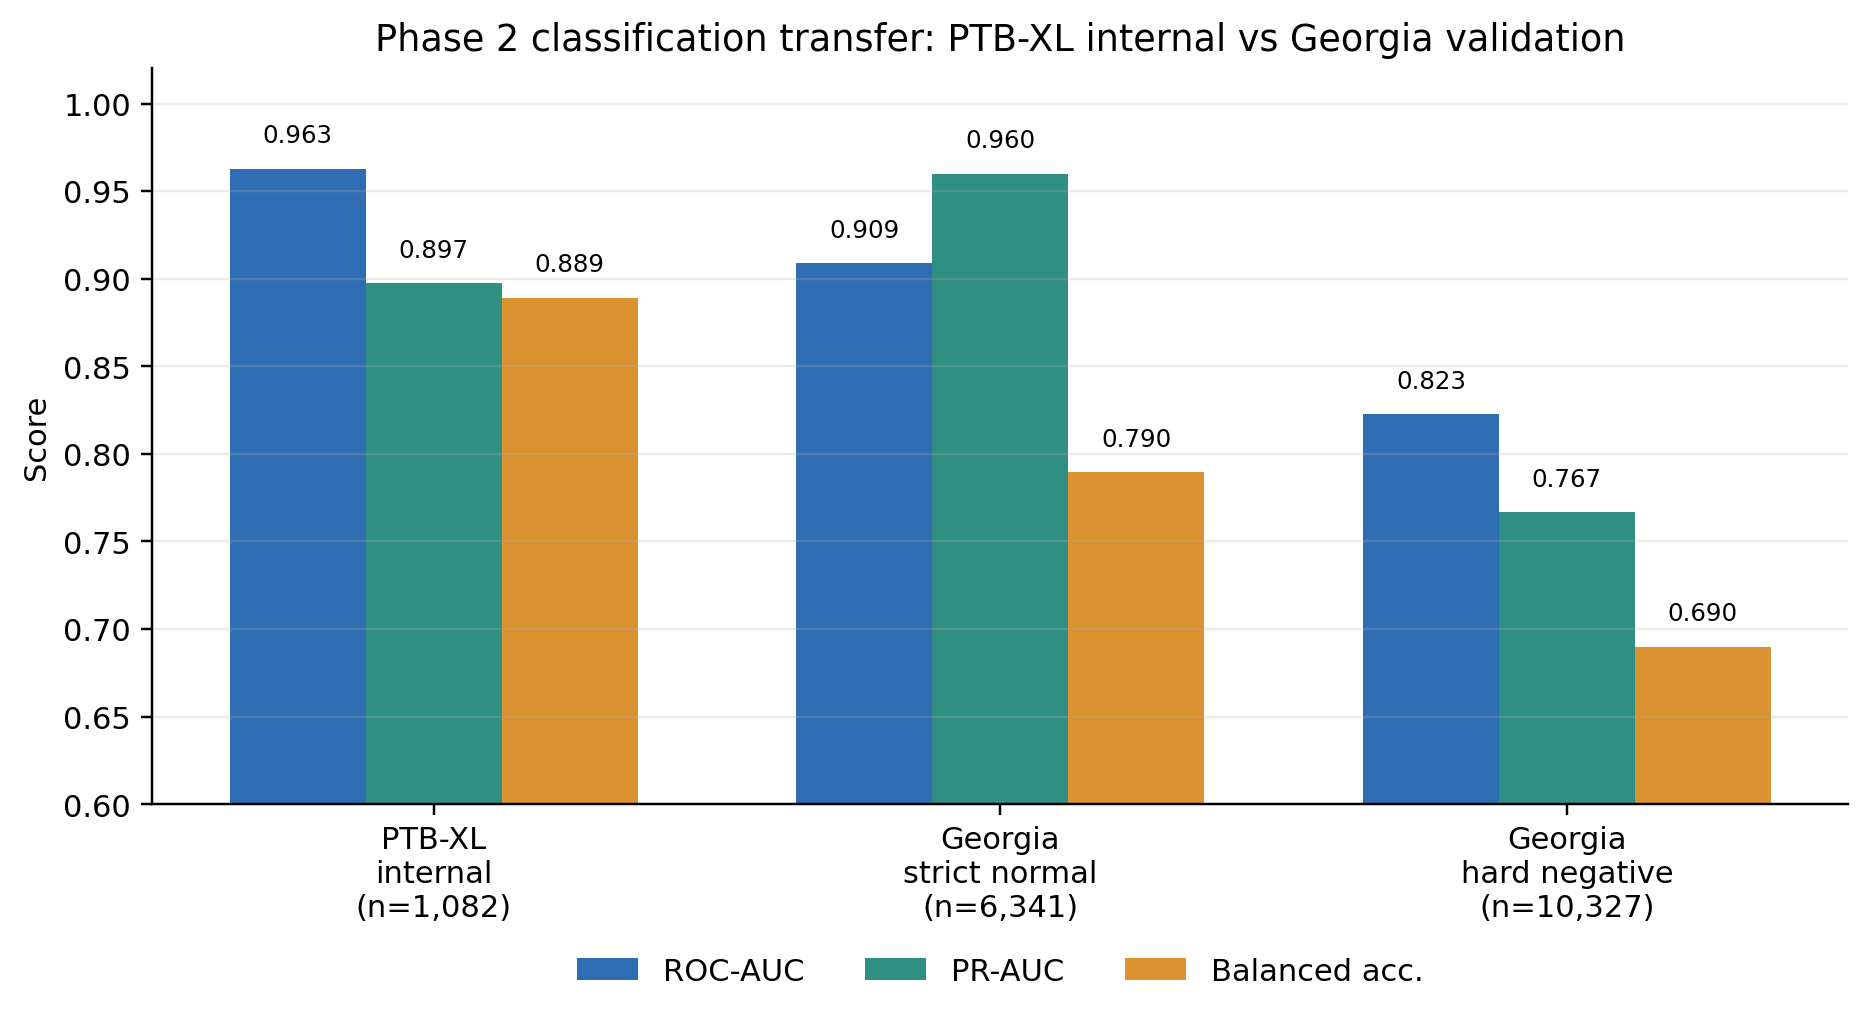
\includegraphics[width=0.86\linewidth]{figure_phase2_external_validation.png}
    \caption{So sánh hiệu năng phân loại của mô hình nền giữa PTB-XL nội bộ và hai cấu hình xác thực ngoại bộ Georgia.}
    \label{fig:phase2_external_validation}
\end{figure}

\blocksep

Các kết quả trên cho thấy khả năng chuyển miền của mô hình phân loại là hữu ích nhưng chưa đủ mạnh để coi là sẵn sàng triển khai, đặc biệt dưới cấu hình âm tính khó. Đây là một ranh giới cần được giữ đúng khi diễn giải kết quả. Tuy nhiên, sự suy giảm của mô hình phân loại không đồng nghĩa với việc cơ chế tín hiệu bị mất hoàn toàn. Vì vậy, ngoài các chỉ số phân loại, cần xem thêm các kết quả phản thực ngoại bộ.

\blocksep

\subsection{Phản thực ngoại bộ trên Georgia}

\blocksep

Trên dữ liệu Georgia dương tính (4\,595 mẫu dương tính đủ điều kiện trích xuất đặc trưng), phản thực mức đặc trưng của cặp \texttt{st\_segment + t\_wave} cho mức giảm xác suất trung bình 0.5034, với tỷ lệ mẫu có xác suất giảm là 97.19\%. Kết quả này phù hợp với hướng và độ lớn quan sát được trên PTB-XL (0.5240).

\blocksep

Ở mức dạng sóng, chỉnh sửa trực tiếp vùng ST/T trên 4\,596 mẫu dương tính của Georgia (bộ dữ liệu đầy đủ, chưa cân bằng) cho mức giảm xác suất trung bình 0.6032, với khoảng tin cậy 95\% từ 0.5941 đến 0.6139. Tỷ lệ đổi nhãn là khoảng 39.06\%, còn tỷ lệ mẫu có xác suất giảm là khoảng 94.56\%. Tương tự PTB-XL, cửa sổ \texttt{pre-QRS} trên Georgia cũng cho hiệu ứng âm, khoảng $-0.0601$.

\blocksep

Quan trọng hơn, chênh lệch giữa ST/T và cửa sổ \texttt{pre-QRS} trên Georgia vẫn duy trì ở mức khoảng 0.6633, gần tương đương với PTB-XL. Điều này khiến \texttt{pre-QRS} trở thành một đối chứng âm tính lặp lại được trên dữ liệu ngoại bộ: không chỉ hiệu ứng mục tiêu còn giữ, mà chính mẫu hình “ST/T dương mạnh còn pre-QRS âm” cũng được tái lập. Đây là bằng chứng có sức thuyết phục, vì nó cho thấy cơ chế mà mô hình sử dụng vẫn có tính chọn lọc theo vùng tín hiệu khi chuyển miền.

\blocksep

Các kết quả này cho thấy hiệu ứng phản thực ST/T không chỉ xuất hiện trên dữ liệu nội bộ mà còn lặp lại trên dữ liệu ngoại bộ. Dù mô hình phân loại giảm hiệu năng ở cấu hình âm tính khó, cơ chế ST/T mà mô hình sử dụng vẫn cho phản ứng cùng chiều và với độ lớn đáng kể trên Georgia.

\begin{table}[H]
\centering
\caption{Tổng hợp phản thực mức đặc trưng và mức dạng sóng trên PTB-XL và Georgia}
\label{tab:phase2_mechanism_summary}
\begin{tabular}{p{0.18\linewidth}C{0.14\linewidth}C{0.14\linewidth}C{0.14\linewidth}C{0.14\linewidth}}
\hline
\textbf{Bộ dữ liệu} & \shortstack{\textbf{Feature-level}\\\textbf{target drop}} & \shortstack{\textbf{Feature-level}\\\textbf{CCS}} & \shortstack{\textbf{Waveform}\\\textbf{ST/T drop}} & \shortstack{\textbf{Waveform}\\\textbf{pre-QRS drop}} \\
\hline
PTB-XL & 0.5240 & 0.3840 & 0.5817 & $-0.0838$ \\
Georgia & 0.5034 & 0.4100 & 0.6032 & $-0.0601$ \\
\hline
\end{tabular}
\end{table}

\noindent\small{Ghi chú: CCS = mean\_prob\_drop của nhóm mục tiêu trừ nhóm đối chứng tốt nhất. Feature-level Georgia được tính trên toàn bộ 4\,595 mẫu dương tính Georgia; nhóm đối chứng tốt nhất là \texttt{global\_morph + beat\_baseline} với 286 đặc trưng và drop = 0.0934. Kết quả waveform-level được lấy từ báo cáo phản thực dạng sóng đầy đủ trên 4\,596 mẫu dương tính Georgia.}

\subsection{Tổng hợp kết quả cơ chế}

\blocksep

Kết quả tổng hợp cuối của pha nghiên cứu thứ hai cho thấy các điểm sau:

\renewcommand{\labelitemi}{$+$}
\begin{itemize}
	\item trên PTB-XL, cặp nhóm mục tiêu \texttt{st\_segment + t\_wave} (247 đặc trưng) cho mức giảm xác suất trung bình 0.5240, trong khi nhóm đối chứng tốt nhất \texttt{global\_morph + beat\_baseline} (286 đặc trưng, lớn hơn nhóm mục tiêu) chỉ cho mức giảm 0.1400; chỉ số CCS đạt 0.3840;
	\item trên Georgia (4\,595 dương tính), cùng cặp mục tiêu \texttt{st\_segment + t\_wave} cho mức giảm 0.5034 và CCS = 0.4100; nhóm đối chứng tốt nhất \texttt{global\_morph + beat\_baseline} (286 đặc trưng, lớn hơn mục tiêu) chỉ cho 0.0934;
	\item phản thực dạng sóng ở cả PTB-XL và Georgia đều cho quan hệ liều -- đáp ứng gần đơn điệu;
	\item đối chứng âm tính \texttt{pre-QRS} đều cho hiệu ứng âm trên cả hai bộ dữ liệu ($-0.0838$ và $-0.0601$).
\end{itemize}

\blocksep

Nếu xét trong phạm vi bài toán ST/T, các kết quả trên hỗ trợ lẫn nhau khá rõ. Mô hình phân loại nền cho hiệu năng nội bộ tốt. Khi kiểm tra bằng phản thực, cả ở mức đặc trưng lẫn mức dạng sóng, vùng ST/T đều cho hiệu ứng mạnh hơn rõ rệt so với các nhóm và cửa sổ đối chứng. Điểm cần nhấn mạnh là nhóm đối chứng mạnh nhất (\texttt{global\_morph + beat\_baseline}, 286 đặc trưng) thậm chí có số chiều lớn hơn nhóm mục tiêu (247 đặc trưng), nhưng vẫn cho mức giảm thấp hơn 3.74 lần trên PTB-XL và 5.39 lần trên Georgia. Điều này cho thấy tác động phản thực đến từ nội dung sinh lý của vùng ST/T, không phải từ kích thước nhóm. Đặc biệt, việc cửa sổ \texttt{pre-QRS} cho hiệu ứng âm trên cả PTB-XL lẫn Georgia là một bằng chứng mạnh cho thấy mô hình không phản ứng đơn thuần với mọi thao tác chỉnh sửa dạng sóng, mà có tính chọn lọc theo đúng vùng tín hiệu mục tiêu.

\blocksep

Hình~\ref{fig:phase2_validation_layers} cho thấy hiệu ứng phản thực mục tiêu được duy trì nhất quán qua hai lớp kiểm chứng: mức đặc trưng và mức dạng sóng. Kết hợp với kết quả xác thực ngoại bộ và đối chứng âm tính \texttt{pre-QRS}, chuỗi kết quả này tạo nên trục bằng chứng chính cho luận điểm ST/T của khóa luận.

\blocksep

\begin{figure}[H]
    \centering
    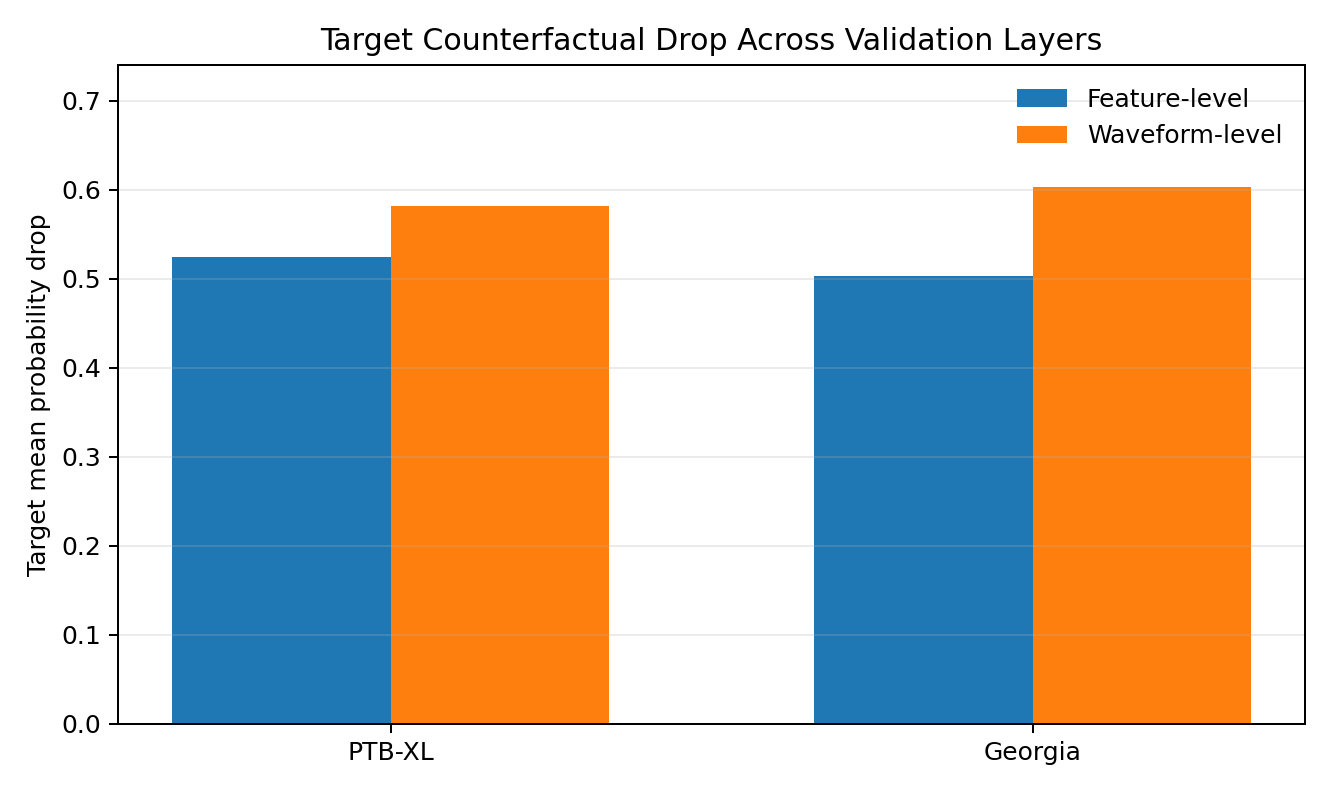
\includegraphics[width=0.80\linewidth]{figure_validation_layers.png}
    \caption{Hiệu ứng phản thực mục tiêu được duy trì nhất quán giữa lớp kiểm chứng mức đặc trưng và mức dạng sóng trên PTB-XL và Georgia.}
    \label{fig:phase2_validation_layers}
\end{figure}

\section{Thảo luận chung}

\blocksep

Khi đặt hai pha nghiên cứu cạnh nhau, có thể thấy chúng phục vụ hai mục tiêu khác nhau nhưng bổ sung cho nhau. Pha nghiên cứu thứ nhất cung cấp một lớp phân tầng nguy cơ CAD trực tiếp từ dữ liệu lâm sàng dạng bảng, với ưu điểm là dễ diễn giải và có thể đánh giá ngoài mẫu tương đối rõ. Pha nghiên cứu thứ hai không nhắm trực tiếp vào nhãn CAD, mà cung cấp một lớp phân tích tín hiệu ECG giúp làm rõ cơ chế bất thường ST/T theo hướng có thể kiểm tra được.

\blocksep

Điểm mạnh của pha thứ nhất là tính minh bạch và tính ổn định của \textit{protective score}. Điểm mạnh của pha thứ hai là thiết kế kiểm chứng cơ chế theo nhiều mức, từ đặc trưng đến dạng sóng, từ dữ liệu nội bộ đến dữ liệu ngoại bộ. Nếu chỉ nhìn riêng từng pha, mỗi pha đều có giới hạn. Tuy nhiên, khi đặt trong phạm vi khóa luận, hai pha tạo thành một cấu trúc hợp lý cho bài toán hỗ trợ đánh giá CAD theo hướng đa nguồn dữ liệu.

\blocksep

Cũng cần xác định rõ ranh giới của kết luận. Từ kết quả của pha nghiên cứu thứ nhất, không thể kết luận rằng \textit{protective score} là một thang điểm lâm sàng sẵn sàng thay thế các quy trình chuẩn. Từ kết quả của pha nghiên cứu thứ hai, càng không thể kết luận rằng mô hình ECG có thể chẩn đoán CAD một cách độc lập. Cách diễn giải phù hợp hơn là: pha thứ nhất cung cấp công cụ phân tầng nguy cơ có thể diễn giải, còn pha thứ hai cung cấp bằng chứng cơ chế cho một mô-đun ECG hỗ trợ đánh giá tim mạch.

\section{Tổng kết chương}

\blocksep

Chương này đã trình bày các kết quả thực nghiệm của hai pha nghiên cứu. Đối với pha nghiên cứu thứ nhất, \textit{protective score} cho thấy quan hệ nghịch rõ với nhãn CAD trên cả ba bộ dữ liệu và có giá trị phân tầng nguy cơ ổn định, dù không tạo ra cải thiện lớn về AUC so với mô hình logistic đối chiếu. Đối với pha nghiên cứu thứ hai, mô hình ECG cho hiệu năng nội bộ tốt trên nhiệm vụ \texttt{NORM vs STTC}; quan trọng hơn, các thí nghiệm phản thực ở mức đặc trưng và mức dạng sóng đều chỉ ra vai trò nổi bật của cơ chế ST/T. Đặc biệt, nhóm mục tiêu \texttt{st\_segment + t\_wave} (247 đặc trưng) cho hiệu ứng phản thực lớn hơn 3.74 lần so với nhóm đối chứng tốt nhất có kích thước lớn hơn (286 đặc trưng), loại trừ khả năng hiệu ứng chỉ đến từ chênh lệch kích thước nhóm. Hiệu ứng này còn lặp lại trên dữ liệu Georgia ngoại bộ.

\blocksep

Từ các kết quả trên, có thể rút ra rằng hướng tiếp cận hai pha của khóa luận là khả thi trong phạm vi bài toán hỗ trợ đánh giá CAD. Pha thứ nhất tạo ra một lớp tri thức lâm sàng dễ diễn giải, còn pha thứ hai tạo ra một lớp bằng chứng tín hiệu có thể kiểm tra. Trên cơ sở đó, chương tiếp theo sẽ tổng kết các kết quả chính của khóa luận, chỉ ra các giới hạn còn tồn tại và nêu một số hướng phát triển tiếp theo.

\newpage
\clearpage
\phantomsection

\addcontentsline{toc}{chapter}{{Kết luận}}
\chapter*{Kết luận}

Bệnh động mạch vành là một bài toán có ý nghĩa thực tiễn cao nhưng cũng có mức độ phức tạp lớn, bởi việc đánh giá người bệnh thường phải dựa trên nhiều nguồn thông tin khác nhau. Xuất phát từ đặc điểm đó, khóa luận lựa chọn tiếp cận bài toán dưới góc nhìn hệ thống hỗ trợ đánh giá đa nguồn dữ liệu thay vì thu gọn toàn bộ vấn đề vào một mô hình đơn lẻ. Trên cơ sở này, khóa luận đề xuất một framework tổng thể và tập trung hiện thực hai thành phần phân tích cốt lõi của framework: thành phần phân tầng nguy cơ CAD từ dữ liệu lâm sàng bằng khai phá luật kết hợp và \textit{protective score}, cùng thành phần kiểm chứng cơ chế ST/T trên ECG bằng bộ nhớ nguyên mẫu phản thực. Nội dung nghiên cứu được triển khai thành hai pha tương ứng với hai thành phần nêu trên.

\blocksep

Đối với pha nghiên cứu thứ nhất, khóa luận đã xây dựng một quy trình khai phá luật kết hợp trên dữ liệu lâm sàng, bao gồm các bước tiền xử lý, rời rạc hóa, mã hóa one-hot, khai phá luật trong từng lần đánh giá chéo và xây dựng \textit{protective score} từ các luật bảo vệ. Kết quả trên ba bộ dữ liệu Z-Alizadeh, UCI Cleveland và UCI Hungarian cho thấy \textit{protective score} có quan hệ nghịch rõ với nhãn CAD và tạo ra sự tách biệt tương đối ổn định giữa nhóm nguy cơ thấp và nhóm nguy cơ cao. Mặc dù việc bổ sung \textit{protective score} vào logistic regression chỉ làm thay đổi diện tích dưới đường cong ROC ở mức rất nhỏ, pha nghiên cứu này vẫn cho thấy giá trị rõ ràng ở góc độ phân tầng nguy cơ và diễn giải lâm sàng.

\blocksep

Đối với pha nghiên cứu thứ hai, khóa luận đã xây dựng thành phần kiểm chứng cơ chế ST/T trên ECG bằng bộ nhớ nguyên mẫu phản thực, trong đó mô hình được huấn luyện trên các đặc trưng ECG 12 chuyển đạo và được kiểm tra bằng nhiều thí nghiệm phản thực. Trên bài toán \texttt{NORM vs STTC} của PTB-XL, mô hình nền đạt hiệu năng phân loại tốt. Quan trọng hơn, các thí nghiệm phản thực ở cả mức đặc trưng và mức dạng sóng đều cho thấy nhóm tín hiệu ST/T, đặc biệt là cặp \texttt{st\_segment + t\_wave}, có ảnh hưởng nổi bật đến quyết định của mô hình. Hiệu ứng này tiếp tục được quan sát trên dữ liệu Georgia ngoại bộ; đồng thời, các đối chứng âm tính và quan hệ liều -- đáp ứng cũng củng cố nhận định rằng mô hình đang dựa vào một cơ chế ST/T tương đối nhất quán.

\blocksep

Nhìn chung, các kết quả thu được cho thấy hướng tiếp cận hai pha là phù hợp trong phạm vi bài toán hỗ trợ đánh giá CAD. Pha thứ nhất cung cấp một thành phần phân tầng nguy cơ từ dữ liệu lâm sàng có khả năng truy vết và diễn giải. Pha thứ hai cung cấp một thành phần phân tích ECG có thể kiểm tra cơ chế tín hiệu bằng phản thực. Hai pha này không thay thế nhau, mà bổ sung cho nhau trong cùng một khung hỗ trợ đánh giá.

\blocksep

Bên cạnh các kết quả đạt được, khóa luận vẫn còn một số hạn chế. Thứ nhất, pha nghiên cứu thứ nhất sử dụng các bộ dữ liệu có quy mô không lớn, đồng thời phụ thuộc vào chất lượng rời rạc hóa và mức độ đầy đủ của các biến lâm sàng. Thứ hai, pha nghiên cứu thứ hai tập trung vào nhãn bất thường ST/T chứ không phải nhãn CAD xác định; vì vậy, kết quả không nên được diễn giải như một hệ thống chẩn đoán CAD chỉ từ ECG. Thứ ba, các phản thực được xây dựng trong không gian biểu diễn và trong khuôn khổ dữ liệu hiện có, nên chưa thể xem như bằng chứng nhân quả sinh lý theo nghĩa chặt. Ngoài ra, hiệu năng ngoại bộ của mô hình phân loại trên cấu hình âm tính khó vẫn suy giảm rõ, cho thấy khoảng cách giữa nghiên cứu cơ chế và khả năng triển khai thực tế còn đáng kể.

\blocksep

Từ các giới hạn trên, một số hướng phát triển tiếp theo có thể được xem xét. Đối với pha nghiên cứu thứ nhất, có thể mở rộng thêm các bộ dữ liệu lâm sàng hoặc chuẩn hóa tập biến đầu vào để kiểm tra tốt hơn tính ổn định của \textit{protective score}. Đối với pha nghiên cứu thứ hai, có thể mở rộng đánh giá sang các bộ dữ liệu ECG độc lập khác hoặc sang các nhãn bệnh tim mạch khác để kiểm tra sâu hơn tính tổng quát của cơ chế ST/T. Trên nền framework hệ thống đã đề xuất, cũng có thể tiếp tục hoàn thiện phần tích hợp báo cáo, quy tắc tổng hợp đầu ra từ hai thành phần và lớp ứng dụng hỗ trợ đánh giá cho người dùng cuối. Đặc biệt, việc tích hợp hai thành phần theo khung quyết định tuần tự có cơ sở nhất định từ y văn: một số nghiên cứu dịch tễ học cho thấy bất thường ST/T trên ECG mang giá trị dự đoán bổ sung độc lập so với điểm nguy cơ lâm sàng dạng Framingham score \cite{StromMoller2007, Badheka2013, Muccini2021}, gợi ý rằng hai nguồn bằng chứng này phản ánh hai khía cạnh bổ sung của cùng một bức tranh sinh lý bệnh và có thể được kết hợp một cách có căn cứ trong các nghiên cứu tiếp theo. Cuối cùng, việc tham khảo ý kiến chuyên gia tim mạch để đối chiếu các kết quả phản thực với lập luận lâm sàng thực tế là một hướng cần thiết nếu muốn đưa nghiên cứu tiến gần hơn tới ứng dụng.

\blocksep

Đối chiếu với bốn mục tiêu nghiên cứu đã nêu ở phần Mở đầu, có thể thấy khóa luận đã đáp ứng được các yêu cầu cốt lõi đã đặt ra. Mục tiêu đề xuất hướng tiếp cận đa nguồn dữ liệu ở mức framework hệ thống đã được hiện thực bằng một khung hai pha, trong đó pha thứ nhất xử lý dữ liệu lâm sàng dạng bảng và pha thứ hai xử lý dữ liệu ECG 12 chuyển đạo. Mục tiêu xây dựng quy trình khai phá luật kết hợp và thang điểm phân tầng đã được triển khai đầy đủ trong pha nghiên cứu thứ nhất, với đánh giá chéo không rò rỉ thông tin và \textit{protective score} cho tương quan nghịch nhất quán với nhãn CAD trên cả ba bộ dữ liệu. Mục tiêu nghiên cứu thành phần kiểm chứng cơ chế ST/T trên ECG bằng bộ nhớ nguyên mẫu phản thực đã được thực hiện thông qua phản thực ở hai mức, đối chứng âm tính và xác thực ngoại bộ trên Georgia. Cuối cùng, mục tiêu đánh giá tính hợp lý, nhất quán và giá trị hỗ trợ chuyên môn của hai pha cũng đã được xem xét qua nhiều lớp bằng chứng bổ sung nhau, từ phân tầng nguy cơ và độ ổn định luật đến hiệu ứng phản thực, quan hệ liều -- đáp ứng và lặp lại trên dữ liệu ngoại bộ.

\blocksep

Tóm lại, khóa luận đã đề xuất một framework hệ thống hỗ trợ đánh giá CAD theo hướng đa nguồn dữ liệu, đồng thời hiện thực và đánh giá hai thành phần phân tích cốt lõi của framework đó. Trong đó, đóng góp của pha thứ nhất nằm ở thành phần phân tầng nguy cơ CAD bằng khai phá luật kết hợp và \textit{protective score}, còn đóng góp của pha thứ hai nằm ở thành phần kiểm chứng cơ chế ST/T trên ECG bằng bộ nhớ nguyên mẫu phản thực. Trong phạm vi của một khóa luận tốt nghiệp, đây là một kết quả có cơ sở, có giới hạn rõ ràng và có thể tiếp tục phát triển trong các nghiên cứu sau.

\newpage

% \appendix
% \input{cover/phu-luc}

\renewcommand{\bibname}{Tài liệu tham khảo}
\clearpage
\phantomsection
\addcontentsline{toc}{chapter}{TÀI LIỆU THAM KHẢO}
\fontsize{13}{16.9}\selectfont

\begin{thebibliography}{99}

\section*{Tiếng Anh}

\bibitem{Agrawal1994}
R. Agrawal and R. Srikant, ``Fast algorithms for mining association rules,'' {\em Proceedings of the 20th International Conference on Very Large Data Bases (VLDB)}, 1994, pp.~487--499.

\bibitem{Alday2021}
E. A. P. Alday, A. Gu, A. J. Shah, C. Robichaux, A. K. I. Wong, C. Liu, F. Liu, A. B. Rad, A. Elola, S. Seyedi, Q. Li, A. Sharma, G. D. Clifford and M. A. Reyna, ``Classification of 12-lead ECGs: The PhysioNet/Computing in Cardiology Challenge 2020,'' {\em Physiological Measurement}, Vol.~41, 2021, pp.~124003.

\bibitem{AlizadehSani2013}
R. Alizadehsani, J. Habibi, M. J. Hosseini, H. Mashayekhi, R. Boghrati, A. Ghandeharioun, B. Bahadorian and Z. A. Sani, ``A data mining approach for diagnosis of coronary artery disease,'' {\em Computer Methods and Programs in Biomedicine}, Vol.~111, 2013, pp.~52--61.

\bibitem{Badheka2013}
A. O. Badheka, N. J. Patel, P. M. Grover et al., ``ST-T wave abnormality in lead aVR and reclassification of cardiovascular risk (from the National Health and Nutrition Examination Survey-III),'' {\em The American Journal of Cardiology}, Vol.~112, 2013, pp.~805--810.

\bibitem{Clifford2006}
G. D. Clifford, F. Azuaje and P. McSharry, {\em Advanced Methods and Tools for ECG Data Analysis}, Artech House, Norwood, 2006.

\bibitem{Conroy2003}
R. M. Conroy, K. Py\"{o}r\"{a}l\"{a}, A. P. Fitzgerald et al., ``Estimation of ten-year risk of fatal cardiovascular disease in Europe: the SCORE project,'' {\em European Heart Journal}, Vol.~24, 2003, pp.~987--1003.

\bibitem{DAgostino2008}
R. B. D'Agostino, R. S. Vasan, M. J. Pencina et al., ``General cardiovascular risk profile for use in primary care,'' {\em Circulation}, Vol.~117, 2008, pp.~743--753.

\bibitem{Detrano1989}
R. Detrano, A. Janosi, W. Steinbrunn, M. Pfisterer, J. J. Schmid, S. Sandhu, K. H. Guppy, S. Lee and V. Froelicher, ``International application of a new probability algorithm for the diagnosis of coronary artery disease,'' {\em American Journal of Cardiology}, Vol.~64, 1989, pp.~304--310.

\bibitem{Diamond1979}
G. A. Diamond and J. S. Forrester, ``Analysis of probability as an aid in the clinical diagnosis of coronary-artery disease,'' {\em The New England Journal of Medicine}, Vol.~300, 1979, pp.~1350--1358.

\bibitem{Guo2017}
C. Guo, G. Pleiss, Y. Sun and K. Q. Weinberger, ``On calibration of modern neural networks,'' {\em Proceedings of the 34th International Conference on Machine Learning (ICML)}, 2017, pp.~1321--1330.

\bibitem{Krittanawong2017}
C. Krittanawong, H. J. Zhang, Z. Wang, M. Aydar and T. Kitai, ``Artificial intelligence in precision cardiovascular medicine,'' {\em Journal of the American College of Cardiology}, Vol.~69, 2017, pp.~2657--2664.

\bibitem{Lavrac1999}
N. Lavra\v{c}, P. A. Flach and B. Zupan, ``Rule evaluation measures: A unifying view,'' in {\em Proceedings of the 9th International Workshop on Inductive Logic Programming (ILP'99)}, Lecture Notes in Artificial Intelligence, Vol.~1634, Springer, 1999, pp.~174--185.

\bibitem{Libby2011}
P. Libby, P. M. Ridker and G. K. Hansson, ``Progress and challenges in translating the biology of atherosclerosis,'' {\em Nature}, Vol.~473, 2011, pp.~317--325.

\bibitem{Lipton2018}
Z. C. Lipton, ``The mythos of model interpretability,'' {\em Communications of the ACM}, Vol.~61, No.~10, 2018, pp.~36--43.

\bibitem{Muccini2021}
C. Muccini, L. Galli, A. Poli et al., ``Exercise ECG for coronary artery disease screening in people living with HIV,'' {\em AIDS}, Vol.~35, 2021, pp.~933--938.

\bibitem{Quinonero2009}
J. Quinonero-Candela, M. Sugiyama, A. Schwaighofer and N. D. Lawrence, {\em Dataset Shift in Machine Learning}, MIT Press, Cambridge, 2009.

\bibitem{Raschka2018}
S. Raschka, ``MLxtend: Providing machine learning and data science utilities and extensions to Python's scientific computing stack,'' {\em Journal of Open Source Software}, Vol.~3, 2018, pp.~638.

\bibitem{Rudin2019}
C. Rudin, ``Stop explaining black box machine learning models for high stakes decisions and use interpretable models instead,'' {\em Nature Machine Intelligence}, Vol.~1, 2019, pp.~206--215.

\bibitem{StromMoller2007}
C. Str\"{o}m M\"{o}ller, B. Zethelius, J. Sundstr\"{o}m and L. Lind, ``Persistent ischaemic ECG abnormalities on repeated ECG examination have important prognostic value for cardiovascular disease beyond established risk factors: a population-based study in middle-aged men with up to 32 years of follow-up,'' {\em Heart}, Vol.~93, 2007, pp.~1104--1110.

\bibitem{Topol2019}
E. J. Topol, ``High-performance medicine: the convergence of human and artificial intelligence,'' {\em Nature Medicine}, Vol.~25, 2019, pp.~44--56.

\bibitem{Wachter2017}
S. Wachter, B. Mittelstadt and C. Russell, ``Counterfactual explanations without opening the black box: Automated decisions and the GDPR,'' {\em Harvard Journal of Law \& Technology}, Vol.~31, 2017, pp.~841--887.

\bibitem{Wagner2020}
P. Wagner, N. Strodthoff, R. Bousseljot, D. Kreiseler, F. I. Lunze, W. Samek and T. Schaeffter, ``PTB-XL, a large publicly available electrocardiography dataset,'' {\em Scientific Data}, Vol.~7, 2020, pp.~154.

\end{thebibliography}

\end{document}
